\documentclass[a4paper,twoside,12pt,nochapterprefix]{scrbook}

\usepackage[utf8]{inputenc}
\DeclareUnicodeCharacter{2500}{\mbox{\vrule height2.2ptdepth-1.8ptwidth.5em}}
\usepackage{amsmath,amssymb,amsthm}
\usepackage[footnotesize,sl,SL,hang,tight]{subfigure}  % helpful package for aligning figures next to each other
\usepackage{longtable} % tables over several pages
\usepackage[font={small,sl},hang,labelfont=bf]{caption} % configure captions
\usepackage{booktabs} % publication quality tables for LaTeX
%\usepackage{showkeys} % shows the labels above the references for easier development

\ifpdfoutput{%
	\usepackage[pdftex]{graphicx}
	\usepackage[]{pdfpages} %for including full pdf pages
}{%
	\usepackage{graphicx}
}

\usepackage{float}
\usepackage{epstopdf}
\usepackage{listings}
\usepackage{color}
\definecolor{lightgray}{rgb}{0.95, 0.95, 0.95}
\definecolor{darkgray}{rgb}{0.4, 0.4, 0.4}
\definecolor{editorGray}{rgb}{0.95, 0.95, 0.95}
\definecolor{editorOcher}{rgb}{1, 0.5, 0} % #FF7F00 -> rgb(239, 169, 0)
\definecolor{editorGreen}{rgb}{0, 0.5, 0} % #007C00 -> rgb(0, 124, 0)
\definecolor{orange}{rgb}{1,0.45,0.13}
\definecolor{olive}{rgb}{0.17,0.59,0.20}
\definecolor{brown}{rgb}{0.69,0.31,0.31}
\definecolor{purple}{rgb}{0.38,0.18,0.81}
\definecolor{lightblue}{rgb}{0.1,0.57,0.7}
\definecolor{lightred}{rgb}{1,0.4,0.5}

%\lstset{
%  basicstyle=\ttfamily\small,
%  columns=fullflexible,
%  frame=single,
%  frameround=tttt,
%  rulecolor=\color{gray},
%}
% http://www.bollchen.de/blog/2011/04/good-looking-line-breaks-with-the-listings-package/
%\lstset{
%  prebreak=\raisebox{0ex}[0ex][0ex]{\ensuremath{\hookleftarrow}},
%  postbreak=\raisebox{0ex}[0ex][0ex]{\ensuremath{\hookrightarrow\space}},
%  breaklines=true,
%  breakatwhitespace=true,
%  numbers=left,
%  numberstyle=\scriptsize,
%}

\lstdefinelanguage{JavaScript}{
	morekeywords={
		break, case, catch, class, const, continue, debugger, default, delete, do, else, enum, export, extends,
		false, finally, for, function, if, import, in, instanceof, new, null, return, super, switch, this, throw,
		true, try, typeof, var, void, while, with, as, implements, interface, let, package, private, protected,
		public, static, yield, any, boolean, constructor, declare, get, module, require, number, set, string,
		symbol, type, from, of
	},
	morecomment=[s]{/*}{*/},
	morecomment=[l]//,
	morestring=[b]",
	morestring=[b]'
}

\lstdefinestyle{TypeScript} {%
	% General design
	%  backgroundcolor=\color{editorGray},
	basicstyle={\footnotesize\ttfamily},
	frame=b,
	% line-numbers
	xleftmargin={0.75cm},
	numbers=left,
	stepnumber=1,
	firstnumber=1,
	numberfirstline=true,
	% Code design
	identifierstyle=\color{black},
	keywordstyle=\color{blue}\bfseries,
	ndkeywordstyle=\color{editorGreen}\bfseries,
	stringstyle=\color{editorOcher}\ttfamily,
	commentstyle=\color{brown}\ttfamily,
	% Code
	language=JavaScript,
	alsodigit={},
	tabsize=2,
	showtabs=false,
	showspaces=false,
	showstringspaces=false,
	extendedchars=true,
	breaklines=true,
	% German umlauts
	literate=%
	{Ö}{{\"O}}1
	{Ä}{{\"A}}1
	{Ü}{{\"U}}1
	{ß}{{\ss}}1
	{ü}{{\"u}}1
	{ä}{{\"a}}1
	{ö}{{\"o}}1
}


\epstopdfsetup{update} % only regenerate pdf files when eps file is newer

\usepackage{rotating} % rotate figures

\usepackage[headinclude]{scrpage2}

% Font packages:
\usepackage{times}
\usepackage{helvet}   % sets sans serif font
\usepackage[T1]{fontenc}

%PDF hyperref config
\ifpdfoutput{%
	\usepackage[pdftex,
		a4paper,
		bookmarks,
		bookmarksopen=true,
		bookmarksnumbered=true,
		pdfauthor={Franz Knobel},       % FILL THIS IN PROPERLY
		pdftitle={Gotscha! - One Way To Support Learning},   % FILL THIS IN PRPERLY
		colorlinks,
		linkcolor=black,
		citecolor=black,
		filecolor=black,
		urlcolor=black,
		anchorcolor=black,
		menucolor=black,
		breaklinks=true,
		pageanchor=true,
		plainpages=false,
		pdfpagelabels=true]{hyperref}
}{}

\ifpdfoutput{%
	\pdfcompresslevel=9
	\pdfoutput=1
	\DeclareGraphicsExtensions{.pdf,.png}
}{}

\bibliographystyle{plain}
%acmsiggraph


% A4
%
\topmargin -0.5in
\textheight 9.3in
\textwidth 6.3in
\oddsidemargin 0.18in
\evensidemargin -0.22in
\parskip 0.1in
\parindent 0in

\renewcommand{\arraystretch}{1.5}
\renewcommand{\baselinestretch}{1}

% !TEX root = ../thesis.tex

% TO DO search symbol
\newcommand{\TODO}{\mbox{\large\bf TO DO}}
\newcommand{\REFR}{\mbox{\large\bf REFR}}

%  Terminates current page and paragraph, makes sure next page starts on
%  an odd-number, and generates a completely blank page, without page markers,
%  if necessary.
\newcommand{\clearemptydoublepage}{\newpage{\pagestyle{empty}\cleardoublepage}}


%% !TEX root = ../thesis.tex

% Stripped from acm siggraph bst and cls
\makeatletter

% no labels in bibliography.
\def\@biblabel#1{}

\newlength{\bibhang}
\setlength{\bibhang}{1em}

% Change in-bibliography biberence style
\def\thebibliography#1{%
  \section*{%
    \bibname\@mkboth{\sl\uppercase{\bibname}}{\sl\uppercase{\bibname}}}
  \list{\relax}{\setlength{\labelsep}{0em}
                \setlength{\itemindent}{-\bibhang}
                \setlength{\leftmargin}{\bibhang}}
  \def\newblock{\hskip .11em plus .33em minus .07em}
  \sloppy\clubpenalty4000\widowpenalty4000
  \sfcode`\.=1000\relax}

% Not sure what this does...
%\def\@citex[#1]#2{\if@filesw\immediate\write\@auxout{\string\citation{#2}}\fi
%  \def\@citea{}\@cite{\@for\@citeb:=#2\do
%    {\@citea\def\@citea{; }\@ifundefined
%      {b@\@citeb}{{\bf ?}\@warning
%      {Citation '\@citeb' on page \thepage \space undefined}}%
%{\csname b@\@citeb\endcsname}}}{#1}}

% Change in-document citation styles
\let\@internalcite\cite
\def\cite{\def\citename##1{##1}\@internalcite}
\def\shortcite{\def\citename##1{}\@internalcite}

\makeatother


\begin{document}

%% Define leading chapter pages
%
% !TEX root = ../thesis.tex

\addtokomafont{chapter}{\setlength{\parskip}{190pt}}   % SEVERE HACK to keep spacing to chapter art work
%\addtokomafont{chapter}{\rmfamily}        % remove this if you prefer sans-serif section titles
%\addtokomafont{section}{\rmfamily}        % remove this if you prefer sans-serif section titles
%\addtokomafont{subsection}{\rmfamily}     % remove this if you prefer sans-serif section titles
%\addtokomafont{subsubsection}{\rmfamily}  % remove this if you prefer sans-serif section titles
%\addtokomafont{paragraph}{\rmfamily}      % replace by \sffamily if you prefer sans-serif para titles
\addtokomafont{paragraph}{\sffamily}

\def\mychpstyleintl{%
{\noindent\setlength{\tabcolsep}{0pt}\setlength{\arrayrulewidth}{2pt}%
\begin{tabular}{c}
\\[100pt]
\begin{tabular}{lr}
\begin{tabular}{p{0.6\linewidth}}
\\
\end{tabular}
&
\begin{tabular}{p{0.4\linewidth}}
\rightline{{%
\sffamily%
\fontseries{bx}%
\fontshape{n}%
\fontsize{100}{120}%choose baselineskip to be 1.2 times font size
\selectfont
\thechapter}}
\end{tabular}
\end{tabular}\\[300pt]
\end{tabular}
}}

\newpagestyle{mychapterpagestyle}{{\protect\mychpstyleintl}{\protect\mychpstyleintl}}{}
\newpagestyle{myappendixpagestyle}{{\protect\mychpstyleintl}{\protect\mychpstyleintl}}{}
%%

%% macros e.g.
\newcommand{\mfytext}[0]{my fancy text}

%refs
\newcommand{\chpref}[1]{Chapter \ref{#1}}
\newcommand{\secref}[1]{Section \ref{#1}}
%\newcommand{\equref}[1]{Equation \ref{#1}} %better use builtin \eqref{}
\newcommand{\figref}[1]{Figure \ref{#1}}
\newcommand{\tabref}[1]{Table \ref{#1}}
\newcommand{\apxref}[1]{Appendix \ref{#1}}
%%

%% Replace this by your own design of a title page
%
%\title{Sound analysis on smartphones}
%\author{Jacqueline Staub}
%\date{March 2014}
%\maketitle
%\clearemptydoublepage
% --- selfmade version ----
\begin{titlepage}
	\topmargin 0.5cm
	\oddsidemargin 0.0cm
	\evensidemargin 0.0cm
	%\textwidth 6.5in
	\centering
	\Huge
	\vspace{1.0cm}
	\textbf{\textsf{Gotscha! - One Way To Support Learning}} \\[1.0cm]
	\includegraphics*[width=0.8\textwidth]{figures/title} \\ % TITLE IMAGE - replace by attractive and representative images from your thesis
	\vspace{1cm}
	\sffamily
	\Large
	Franz\ Knobel
	\\[0.8cm]
	\large
	Bachelor\ Thesis
	\\
	\today
	\\[1.3cm]
	\emph{Supervising Professor:}\\
	Prof.\ Dr.\ Juraj Hromkovi\v c		% The supervising professor
	\\[0.8cm]
	\emph{Supervisor:}\\
	Elizabeta\ Cavar
	\vfill
	\includegraphics*[height=0.8cm]{figures/eth_logo_kurz_pos.eps} \hfill
	\vspace{3.4cm}
\end{titlepage}
\clearemptydoublepage
%%

\pagenumbering{roman}
\setcounter{page}{1}

% !TEX root = ../thesis.tex

\chapter*{Abstract}

As the importance of computer science is rising, certain games that support the
developement of abstract thinking, analytical skills and decision making, are
becoming more and more interesting at an early age. Through identification and
describing relationships between items, children develop a foundation to early
math skills and basic concepts of computer science (e.g. combinatorics of finite
affine and projective spaces, the theory of error-correcting codes, hashing, etc.)
\cite{SET}. The pupils individual learning speed and lack of concentration, if
not receiving the right amount of attention, is another challenge by itself.
Without individual fostering, children are at high risk of losing interest.
Through this thesis the teachers will be introduced to a tool for their pupils.
Focused on classification of objects with certain properties, the pupils get
introduced to a computer-based learning environment. There they can individually
train and improve themselves in this field. In the mean time the teachers can
concentrate on the majority of their pupils and have the opportunity to work with
pupils on an individual basis, without feeling the pressure of having to support
everyone at once.
It has shown, that gamification has enormous potential. It takes time to learn how
to create games. Once overcome, creating further games is not as hard as one may think.
In the created test environment the test subjects have shown more concentration,
individual work behaviour and more willingness to learn than in the whole group.
Keywords : phaser 3, typescript, debugging, testing, from a topic to the game, how to tackle a new framework

% !TEX root = ../thesis.tex

\chapter*{Acknowledgment}

I want to thank my supervisor Elizabeta Cavar for supporting me in the last six months.
Without her input and constant reminder of our deadlines, I would have had a lot more obstacles on the way.
Also many thanks to Jaqueline Staub, Nicole Trachsler and Philippe Voinov for their help with specific topics on my work.
Another very important role in my work played the debuggers, the ones who tested my program and searched for any kind of problems.
Thank you for your time, effort and fun you had with my work:
Dilana Kunz, Guido von Burg, Julia Badertscher, Ronja Koeppel, Jonathan Chen


%-----------------------------------------------------------------------------------------------
%include task description here:
\cleardoublepage
%\includegraphics[viewport=3cm 0cm 20cm 27.5cm]{task_description} %better use includepdf below!
%\includepdf{task_description}
\cleardoublepage
%-----------------------------------------------------------------------------------------------

ib%include acknowledgment here:
%% !TEX root = ../thesis.tex

\chapter*{Acknowledgment}

I want to thank my supervisor Elizabeta Cavar for supporting me in the last six months.
Without her input and constant reminder of our deadlines, I would have had a lot more obstacles on the way.
Also many thanks to Jaqueline Staub, Nicole Trachsler and Philippe Voinov for their help with specific topics on my work.
Another very important role in my work played the debuggers, the ones who tested my program and searched for any kind of problems.
Thank you for your time, effort and fun you had with my work:
Dilana Kunz, Guido von Burg, Julia Badertscher, Ronja Koeppel, Jonathan Chen


\tableofcontents

\cleardoublepage

\pagenumbering{arabic}
\renewcommand*{\chapterpagestyle}{mychapterpagestyle}
\renewcommand*{\chapterformat}{} % show chapter titles only (no numbers)
% \setchapterpreamble[o]{...}  unfortunately does not move the \chapter output downwards

% ---- MAIN PART ----


% !TEX root = ../thesis.tex

% set counter to n-1:
\setcounter{chapter}{0}

\chapter{Introduction}\label{ch:introduction}
\section{Introduction}\label{sec:introduction}
The importance of computer science is rising.
The development of abstract thinking, analytical skills and decision-making,
are becoming more and more interesting at an early age.
Through identification and describing relationships between items,
children develop a foundation to early math skills and basic concepts of computer science
(e.g.\ combinatorics of finite affine and projective spaces, the theory of error-correcting codes, hashing, etc.)\cite{cardgameset}.
The pupils individual learning speed and lack of concentration,
if not receiving the right amount of attention, is another challenge by itself.
Without individual fostering, children are at high risk of losing interest.
Through this thesis the teachers will be introduced to a tool for their pupils.
Focused on classification of objects with certain properties, the pupils get introduced to a computer-based
learning environment or so called game based learning.
There they can individually train and improve themselves in this field.
In the meantime the teachers can concentrate on the majority of their pupils and have the opportunity to work with
pupils on an individual basis, without feeling the pressure of having to support everyone at once.

\section{Goals of the Thesis}\label{sec:goals-of-the-thesis}
The main objective of this thesis consists of planning, analyzing, implementing
and testing a computer-based learning environment on the topic of
classification. The student studies the already existing implementations of
"INFORMATIK BIBER in KG und 1/2", analyses the capabilities of kindergarten kids
and first graders, develops an interactive classification tool, implements it
then on a platform compatible with the implementation of "INFORMATIK BIBER in KG
und 1/2"\cite{ibkg12} and conducts an evaluation with test subjects.
The implementation is going to be integrated into the existing system of "Einfach Informatik"\cite{einfachinformatik}.
The outcome of this thesis is a well-documented, stable and
reliable prototype, providing the functional elements to be used in schools.

\section{Problem Statement}\label{sec:problem-statement}
Concerning computer science in schools, new educational material is in production and some is already distributed.
With the printed teaching materials, the need for digitalized materials and exercises will come.
In related work [\ref{ch:relatedwork}] the already published digitalized exercises and
in which way they were realized is addressed.
The book \textit{"INFORMATIK BIBER in KG und 1/2"}\cite{ibkg12} was published recently and only parts have been digitalized yet.
In this thesis the part where children learn how to identify and compare properties of different objects is covered.

The focus though will not solely lie on the translation of the existing teaching material to a
computer-based learning environment, but also on introducing learning methods in a gamified environment which
not only complements the teachers with their teachings but also assisting them.

The main questions we are going to ask are:

\begin{itemize}
    \item How can we reach and support our target audience?
    \item What is our target audience capable of?
    \item What kind of different digital environments are there?
\end{itemize}

\section{Background}\label{sec:background}
The key contribution of computer science to general school education is rooted in the concept of
\textit{algorithmic thinking}\cite{HKKS17}.
One way of introducing kindergarten and primary school pupils to algorithmic thinking and
it's concepts consists in making them solve problems with and without computers.
This can be achieved using age- and knowledge-appropriate learning materials.

\section{Motivation}\label{sec:motivation}
Computer science provides already an easier way than other topics for teaching in the digitalized world.
As one can at least guess the huge potential to make use of the students daily enjoyments while still teaching
them the necessary things, it would be a loss to the teaching world not to explore and evaluate this kind of teaching
method. Especially game based learning as gamified learning is already being explored and evaluated.
The aspect of integrating this method as a helper/assistant to the teacher and not only as an additional feature in
their free time, is alone very tempting to explore in my opinion.

\section{Outline}\label{sec:outlook}
In the following chapters related work in the field of game based learning will be addressed,
and the target audience as well as electronic devices will be analyzed for their requirements and capabilities.
Furthermore, the created learning environment based on game based learning is explained in detail, its evaluation and
future applications and improvements.

% !TEX root = ../thesis.tex

% set counter to n-1:
\setcounter{chapter}{1}

\chapter{Related Work}\label{ch:relatedwork}
In this section we are going through some previous works in a the same area.
Starting with mainly publications, in a second part we take look at gamification
and game based learning and in a third part we look at existing educational software
and highlight their pros and cons to build on the experiences made there.

\section{Previous work}\label{sec:previous-work}
Several papers with corresponding online learning environments based on the teaching materials "Einfach Informatik"\
\cite{ei56, ei79dat, ei79strat} have been proposed by ETH Students\ \cite{stblum, skamp, tangk, jweber}.

The learning environments they created/extended are mainly based on adding gamification elements to digitalized tasks
instead of creating a game based environment.
This works to some extent as the texts and exercises can be used from the book.

Their environment is based on TypeScript, the Angular framework and accessible through the homepage \textbf{Einfach Informatik}\cite{einfachinformatik}.

It contains a lot of information for both students and teachers.
Information about the task is mainly obtained via text.
Thus one requirement is being able to read or being accompanied by someone who is able to.

Often teacher can upload exercises or create tasks.
This can be seen as a disadvantage as then the teacher has to focus on doing something other than care for the majority
of his class.

Exercises are sorted by textbook chapter, which is in my opition a valid strategy to use the learning environment as an
addition to the textbook.
Each topic contains exercises, as well as exams, where students can solve
them and sum up the skills they were supposed to acquire in this chapter.
The division of the exercises into different difficulty levels offers each student level adjusted exercises by knowing
in advance which exercises require a basic level of understanding and which ones are for the more advanced students.
The main goal tries to focus on the engagment of the students interest on the subject which is good.

\subsection{Angular}\label{subsec:angular}
Angular is an open-source web application framework based on TypeScript.
It is maintained by Google and offers lots of built-in functionalities.
It uses HTML and CSS for the view of the application and TypeScript for the model and the controller.
As Google is supervised the framework, it is contiguously developed and tested,
which makes it a stable Framework giving lots of hands for fast development.

\section{Gamification and Game Based Learning (GBL)}\label{sec:gamification-and-game-based-learninggbl}
\subsection{Gamification}\label{subsec:gamification}
Gamification reflects a social phenomenon arising with a generation of digitally literate population.
It has been defined as the use of "game-based mechanics, aesthetics, and game thinking to engage people,
motivate action, promote learning, and solve problems"\cite{kapp2013gamification}.
This includes digital game mechanics, but is not limited to, avatars, badges, points, levels,
leaderboard, virtual rewards, and storyline or even quests.
There is also an aspect to game elements that allow for social interaction between players and the aquisition of
critical thinking skills, which are essential in learning.

Digital video game elements that are used in the pedagogical context promote task engagement, increase motivation,
and enforce desirable learning behaviour.
The rationale behind deploying video game elements in an educational context is that they have already captured the
attention of millions of people all over the world.

\subsection{Game-Based-Learning}\label{subsec:game-based-learning}
Game based learning describes an approach to teaching,
where students explore relevant aspects of games in a learning context.
Generally, it is designed to balance subject matter with gameplay and the ability of the player
to retain and apply said subject matter to the real world.

Good game-based learning applications can draw the user into virtual environments that look and feel familiar and relevant.
Within an effective game-based learning environment, it is common to work towards a goal,
choosing actions and experiencing the consequences of those actions along the way.
Making mistakes in a risk-free setting, and through experimentation,
it is actively learned and practiced the right way to do things.
This keeps the user highly engaged in practicing behaviors and thought processes that he can easily transfer from the
simulated environment to the real life\cite{gal}.

\subsection{Gamification vs. Game-Based-Learning}\label{subsec:gamification-vs.-game-based-learning}
While game based learning is similar to gamification, it is a different breed of learning experience.
Gamification takes game elements and applies them to a non-game setting.
Game based learning is designed to balance subject matter with gameplay and the ability of the player to retain,
and apply said subject matter to the real world.

\section{Existing Educational Software}\label{sec:existing-educational-software}
The idea of propagating games based on game based learning is often touched but rarely integrated in schools.
Sometimes they have more in common with normal computer games and the learning aspect is only discovered when specific looked at.
En good example of a such company is the learning company\cite{tlc}.

The learning company produced a grade-based system of learning software and tools to improve productivity.
It was known for its games like Reader Rabbit\cite{readerrabbit} and OutNumbered!\cite{outnumbered}.

Reader Rabbit is an educational game franchise and a series aimed at children from infancy to the age of eight.

OutNumbered! is an educational computer game software aimed at children ages seven to fourteen and
is designed to teach children mathematical computation and problem solving skills.

Both games have a storyline with a specific designed environment which includes minigames and challenges covering
various topics not only focusing on one subject.

The games teach language arts including basic skills in reading and spelling, and mathematics.
They are designed to be played alone and not as an addition to the lessons at school but as additional homework or
recreational activities over the holidays to not forget the freshly learned subjects.

It had great success depending on the perspective, as the kids were sitting at the computer over the holidays in summer
and "learning" instead of playing outside. Kids see such games as what the games are trying to be, games without noticing
the learning aspect. Though, it is difficult to create one game for a broad spectrum of users, as the level of the topics
vary from country to county or even town to town. This becomes even more complicated if multiple topics from different
school subjects are included in one game. If a part of a game is too easy or too hard for the user you are risking
loosing his attention fast, depending on his the age.

In my opinion the rise and fall of those games was on one hand the integrated learning process in a story and minigames which
were very satisfying to the normal user, as he did not notice that he was learning.
Unfortunately, the games were not supporting the teacher in class and only supplementary.
Why should I play a game related to school when there are multiple other games with better gameplay,
a more interesting storyline and better visual effects?
Yes, it is nearly impossible to compete with the game industry if you are not , but if you cannot compete, change the playfield.
The playfield normal games will never touch is the school, as they normally have no correlation to school topics.

% !TEX root = ../thesis.tex

\chapter{Requirements}\label{ch:requirements}
In this section we will capture the requirements for our learning environment.
We will look into the cognitive and motor abilities of the target audience and
some elements of gamification which will be analyzed and assessed.
The existing environment, our work should be implemented in, has conditions as well.
Those will be taken into consideration while evaluating a suitable framework.

\section{Programming Environment}
\subsection{Boundary Conditions}
\begin{itemize}
    \item The game should be maintainable as it is not excluded that others are going to work on it.
    \item Modularity is an important aspect as one cannot assume the final design to this point in time.
    \item It should be possible to integrate it in a Typescript/JavaScript/HTML environment (e.g.\ as a canvas) as
    all similar work up until now is mostly written in Typescript
    \item The ability to run on computers and tablets is important as a lot of schools have one or the other.
    \item Easy to learn. Support is an important aspect as it is easier to start with something new.
    A huge community correlates in most cases with good support on free open source software.
\end{itemize}

\subsection{Evaluation of Possible Solutions}
\subsubsection{Babylon.js}
Babylon.js is a complete JavaScript framework for building 3D games.
Using WebGL for graphics, the feature set for Babylon is somewhat extensive.
Its community is said to be fairly active.
The most significant features are:

\begin{itemize}
    \item Support and exporting tools
    \item Game engine staples such as scene picking, collision handling, and scene graphs
    \item Particle and animation systems
    \item Performance optimizations such as frustum clipping, hardware scaling, and occlusion queries
    \item Shader, rendering, and texture systems
    \item Expansive mesh support
\end{itemize}

Babylon does not require to be installed as an internal entity on your computer.
Thus, all development can happen within the browser/code editor itself\cite{phaserad}.

\subsubsection{Pixi.js}
Pixi.js is a 2D game rendering engine intended for HTML5 games.
There are benefits of its integrated hardware acceleration.
Pixi’s focus lies not on WebGL, yet utilizes rich game content, interactive displays,
and apps that are supported on all platforms equally.
It is said that it is the way that Pixi has been built that enables for it to be a smooth, rapid, and evenly interactive rendering engine\cite{phaserad}.

\subsubsection{Melon.js}
Melon.js has a sprite-built JavaScript engine for 2D game development,
is an independent project which does not require additional libraries to work,
supports mobile type devices as well as all leading browsers,
optimization for mobile devices for motion and hardware,
in-built HTML5 audio support,
a practical physics engine to reduce the CPU usage,
a great deal of effects that would be required for creating a
functional on-line game in the browser.
Community forums is hosted on Google Groups, where you can quickly yield answers to your questions in regards to how Melon.js works or in the case of you experiencing bugs.
The documentation features several dozens of demo applications built with Melon,
some of which are open-source and can be used to learn different aspects of game development from\cite{phaserad}.

\subsubsection{Phaser}
Phaser is a free and open source JavaScript/TypeScript framework which puts a focus on letting coders make games quickly.
The system works primarily with Canvas and WebGL, letting programmers easily build substantial games for both
desktop and mobile browsers.

It is said that phaser has an active community that regularly participates on the forum, Slack, and Discord channels.

One of the biggest benefits of this engine is that it is a fully-featured engine,
so it isn’t restricted to doing just one thing.
Here’s a list of some of the feature sets provided with Phaser:

\begin{itemize}
    \item built on WebGL and canvas
    \item preloader system
    \item physics features
    \item sprite and animation handling
    \item particle system
    \item camera, input, and sound systems
    \item tilemap support
    \item device scaling support
    \item plugin availability
\end{itemize}

Phaser’s preloader makes it easy for developers to load their game assets and have them automatically handled.
That way, you don’t have to waste time writing extensive code for each part of the game\cite{phaserad}.

\subsubsection{Evaluation of the Frameworks}
Through the boundary conditions one can see that the TypeScript support, a lot of code examples,
an active community for support and multiple browser support is most important for this work.
After a short evaluation of the most featured JavaScript/TypeScript game engines, it became clear,
that the phaser framework fulfils our conditions to a fairly good extent.

\section{Boundary Conditions of the problem statement}
There have to be objects with different property categories with multiple properties in each category.
With these objects should be played with in different levels of difficulty.
There should be easy levels for inexperienced users and hard levels for more advanced users.
The aspect of hashing in the context of sorting these objects with limited available space must be included.

\section{Target Audience}
The target audience are going to be children between the age of 5 and 8.
They cannot be expected to be able to read or write. Numbers from 1 to 5 should be possible though.
The motoric abilities of children with tablets are rather advanced in contrast to useing a computer with a mouse.
So a touch screen of any kind is not a problem but the handling with a keyboard of a mouse cannot be assumed.

\section{Elements of Gamification}
\begin{itemize}
    \item Easy levels for beginners
    \item Hard levels for experienced users
    \item Levels should always be playable under difficult conditions to strengthen what you have learned
    \item Reward system for instant gratification and progress tracking
    \item The gratification should be visualized
    \item Tracking of correct and incorrect choices made
    \item Time limits
    \item Sound
    \item If possible there should be an aspect of a story/timeline
    \item A fullscreen option helps to stay focused
    \item A level manu or a map
\end{itemize}
\section{Additional Conditions}


Objects should have properties and subproperties.

Game
- capturing name
- objects categories nad subcategories
- easy level
- easy level under harder difficulties
- limited sorting -> hashing
- set easy
- set hard
- overview
- gamification
    - track progress
        - time based
        - correct and wrong
        - visual gratification
    - have fun dont recognize you are learning
        - optics
            - randomization and more options for variety
        - sound
        - story like
    - menu
    - levelmenu
    - fullscreen
    - flow
        - exitbutton
        - returnbutton

% !TEX root = ../thesis.tex

\chapter{Design of the Learning Environment}
\label{chap:design}

In this section all implementation tools and approaches are explained.
First our used framework will be explained, then how our different scenes and objects are generated and
at last how these two are combined to our final solution: Gotscha!
Gotscha is a learning environment based on game based learning.
The user goes through multiple levels to learn detecting and comparing properties of objects
under simple and more difficult situations.

\section{Phaser 3}\label{sec:phaser-3}
%https://labs.phaser.io/
%https://phaser.io/
%https://photonstorm.github.io/phaser3-docs/

Phaser [\ref{TODO}] is an open source HTML5 [\ref{TODO}] game framework created by Photon Storm [\ref{TODO}].
It is a JavaScript/TypeScript [\ref{TODO}] library designed to run on all major desktop browsers.
A lot of focus was given to the performance inside of mobile web browsers.
Important for the renderer is that if the device is capable, it uses WebGL [\ref{TODO}], otherwise it seamlessly reverts to Canvas [\ref{TODO}].
The current version is 3.17 and is used in this work. Version 4 is currently in development.

\subsection{Base Configuration}\label{subsec:base-configuration}
In Phaser 3, games need a configuration file and a starting point.

For example:
\begin{lstlisting}[style=TypeScript, caption={Game Setup File}]
    import 'phaser';
    import GameConfig = Phaser.Types.Core.GameConfig;
    import RenderConfig = Phaser.Types.Core.RenderConfig;
    import {Scene1} from './scene1';
    import {Scene2} from './scene2';

    // Defining the renderer
    const renderConfig: RenderConfig = {
        antialias: true,
        pixelArt: false
    };

    // Enforcing widescreen
    let width: number = window.screen.width;
    let height: number = window.screen.height;

    if (window.screen.width <= window.screen.height) {
        width = window.screen.height;
        height = window.screen.width;
    }

    // Game Configuration
    const config: GameConfig = {
        title: 'TITLE',
        parent: 'game',
        type: Phaser.AUTO,
        scene: [
            scene1, scene2
        ],
        physics: {
            default: 'arcade',
            arcade: {
                debug: false
            }
        },

        // Master background color
        backgroundColor: '#000000',

        render: renderConfig,

        scale: {
            parent: 'phaser-example',
            mode: Phaser.Scale.FIT,
            autoCenter: Phaser.Scale.CENTER_BOTH,
            width: width,
            height: height
        }
    };

    export class GameName extends Phaser.Game {
        constructor(config: GameConfig) {
            super(config);
        }
    }

    // Event handler for starting the game
    window.onload = () => {
        const game = new GameName(config);
    };
\end{lstlisting}

\subsection{Scenes}\label{subsec:scenes}
Games in Phaser 3+ are structured around scene objects.
A scene is a collection of game objects and related logic because these two should be kept together.
The objects will be drawn when the scene is rendered.

Where this gets special is that Phaser doesn't place any constraints on how many scenes need to be running.
This means you can have 0, 1, or as many as you need running at once.
You can communicate between them and each scene has a depth (z-index).
With the z-index a UI scene, rendered above the play scene, which is always rendered above the background scene, is possible.

\subsubsection{Lifecycle}
A simplified model has a scene that moves between four states: \textit{Create, Update Loop, Paused, and Stopped}.
Transitions are initiated by a function call and emit a signal that can be listened for.
This way, you can take action at specific point in the process.

The scene state transitions and fired events are summarized in the following state diagram.
Functions which initiate a transition are in yellow and signals emitted are orange.

\begin{figure}[H]
    \centering
    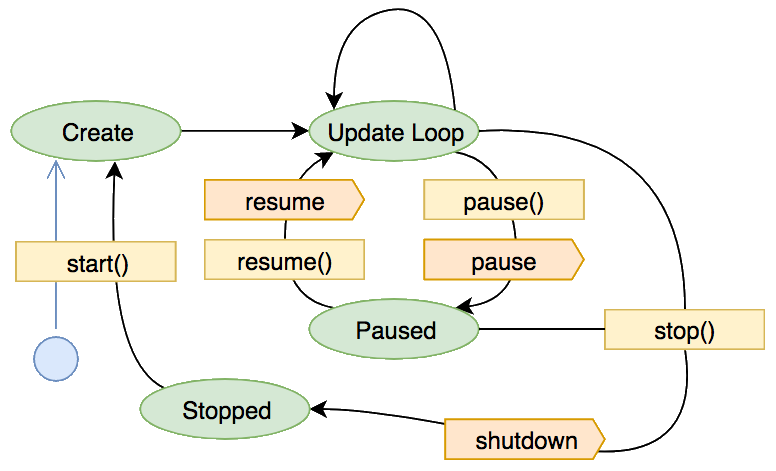
\includegraphics[width=0.8\textwidth]{figures/lifecycle}
    \caption{Scene Lifecycle [\ref{TODO}]}
    \label{fig:lifecycle}
\end{figure}

An interesting behavior is that once a scene has been shut down it is not garbage collected.
The scene can always be resumed by the start() method.
When this happens the three creation functions get called once more.
This means any state tracked in the scene class will be retained between a stopped state and the next create state.
Thus special care must be taken to set a known initial value on everything requiring one.
Especially when loading/creating objects outside the preloader (animations, tweens, audiofiles, etc.).

Scenes here have 5 functions:

\begin{itemize}
    \item \textbf{constructor()}: Run 1 time.
    \item \textbf{init()}: Run 1 time. Initialization of fields and passed on data by other scenes.
    \item \textbf{preload()}: Run 1 time. Loads up all the assets inside the scene like images and audio.
    \item \textbf{create()}: Run 1 time. Position and display the assets that are already preloaded, animations, physics, etc.
    \item \textbf{update()}: Run 1 time per frame, takes care of everything related to the game logic.
\end{itemize}

\subsection{Managers}\label{subsec:managers}
In Phaser 3 managers are a global system.
Animations, scenes, images loaded/created within it are globally available to all game objects.
They share the base data while managing their own timelines.
This allows the definition of a single object once and its application to as many game objects as required.
So a game object can be called in an completely other and unrelated scene.
Examples for used managers in this work are:

\begin{itemize}
    \item \textbf{Scene Manager} (scene.scenes). Contains all scenes of the game once created.
    \item \textbf{Texture Manager} (scene.textures). Contains all textures once loaded.
    \item \textbf{Audio Manager} (scene.sound). Contains all audio files once loaded.
    \item \textbf{Data Manager} (scene.data). Shared data manager.
    An event (listenable) is triggered when an event is stored/changed.
    \item \textbf{Cache Manager} (scene.cache). Contains all special files once loaded.
    \item \textbf{Animation Manager} (scene.anims). Contains all animations once created.
    \item \textbf{Tween Manager} (scene.tweens). Contains all tween objects once created.
    A Tween is able to manipulate the properties of one or more objects to any given value, based
    on a duration and type of ease.
\end{itemize}

\section{Object Generation}\label{sec:object-generation}
Our objects can have up to four properties with exactly one from each of the following categories:

\begin{itemize}
    \item \textbf{Geometrical shape} (square, triangle, circle, ellipse, rhombus, octagon)
    \item \textbf{Color} (yellow, orange, red, purple, green, blue)
    \item \textbf{Holes} or dots (one, two, three, four, five, six)
    \item \textbf{Filling} (filled, striped, dotted)
\end{itemize}

All possible objects with one, three and four properties, are needed.

With a python script [\ref{lst:svggen}] scalable vector graphic (SVG) [\ref{TODO}] files are generated [\ref{lst:svgimagefile}].
After that they are converted to portable network graphic (PNG)[\ref{TODO}] files with the GNU image manipulation program (GIMP) [\ref{TODO}].
Additional image scaling and cropping is done for saving space and only displaying the actual image with as less empty space as possible around it.
With the imagemagick command mogrify [\ref{lst:mogrify}] the last step is easily applicable to all 1000+ images.

\begin{lstlisting}[style=TypeScript, caption={ImageMagick console command "mogrify"}, label={lst:mogrify}]
    mogrify -resize 50% -trim -repage *.png
\end{lstlisting}

\begin{lstlisting}[style=TypeScript, caption={SVG Generation}, label={lst:svggen}]
    ...
    imageString = imgStr(colordefault, colordark, square, circle, triangle, ellipse, octagon, rhombus, filling, one,
                         two, three, four, five, six)

    filename = colordefault + shape + number + fillingname

    with open("images/svg/" + filename + ".svg", "w+") as file:
        file.write(imageString)
        file.close()
    ...
\end{lstlisting}

\begin{lstlisting}[style=TypeScript, caption={SVG Image File}, label={lst:svgimagefile}]
    <?xml version="1.0" standalone="yes"?>

    <svg height="1000" width="1000" viewbox="0 0 1000 1000" xmlns="http://www.w3.org/2000/svg">
    <defs>
            <pattern id="stripe" patternUnits="userSpaceOnUse" width="20%" height="20%">
                <path stroke="aqua" stroke-linecap="butt" stroke-width="50" d="M -20 -20 l1000 1000"/>
                <path stroke="aqua" stroke-linecap="butt" stroke-width="50" d="M -20 180 l1000 1000"/>
                <path stroke="aqua" stroke-linecap="butt" stroke-width="50" d="M -20 -220 l1000 1000"/>

            </pattern>
            <pattern id="dotted" enable-background="true" patternUnits="userSpaceOnUse" width="15%" height="15%">
                <circle cx="30" cy="30" r="25" fill="aqua" />
                <circle cx="105" cy="105" r="25" fill="aqua" />
            </pattern>
            <style>
            .button {

            stroke-width:5;
            stroke:black;

            }
        </style>
        </defs>

     <g id="circle" display="none">
         <circle cx="500" cy="500" r="300" class="button" fill="blue"/>
         <circle cx="500" cy="500" r="300" class="button" fill="none"/>
         <circle cx="500" cy="500" r="250" class="button" fill="none"/>
     </g>

     <g id="square" display="inherit">
      <rect x="250" y="250" rx="20" ry="20" width="500" height="500" class="button" fill="blue"/>
      <rect x="250" y="250" rx="20" ry="20" width="500" height="500" class="button" fill="none"/>
      <rect x="300" y="300" rx="20" ry="20" width="400" height="400" class="button" fill="none"/>
     </g>

     <g id="triangle" display="none">
      <polygon points="500,50 113.4,700 886.6,700" stroke-linejoin="round" class="button" fill="blue" />
      <polygon points="500,50 113.4,700 886.6,700" stroke-linejoin="round" class="button" fill="none" />
      <polygon points="500,150 200,650 800,650" stroke-linejoin="round" class="button" fill="none"/>
     </g>

     <g id="ellipse" display="none">
      <ellipse cx="500" cy="500" rx="400" ry="250" class="button" fill="blue" />
      <ellipse cx="500" cy="500" rx="400" ry="250" class="button" fill="none" />
      <ellipse cx="500" cy="500" rx="350" ry="200" class="button" fill="none" />
     </g>
     <g id="octagon" display="none">
      <polygon points="400,250 600,250 750,400 750,600 600,750 400,750 250,600 250,400" stroke-linejoin="round" class="button" fill="blue" />
      <polygon points="400,250 600,250 750,400 750,600 600,750 400,750 250,600 250,400" stroke-linejoin="round" class="button" fill="none" />
      <polygon points="400,300 600,300 700,400 700,600 600,700 400,700 300,600 300,400" stroke-linejoin="round" class="button" fill="none"/>
     </g>

     <g id="rhombus" display="none">
      <polygon points="350,250 150,750 650,750 850,250" stroke-linejoin="round" class="button" fill="blue" />
      <polygon points="350,250 150,750 650,750 850,250" stroke-linejoin="round" class="button" fill="none" />
      <polygon points="390,300 230,700 620,700 770,300" stroke-linejoin="round" class="button" fill="none"/>
     </g>


     <g id="one" display="none">
      <circle cx="500" cy="500" r="40" stroke="black" fill="black"/>
     </g>

     <g id="two" display="none">
      <circle cx="570" cy="500" r="40" stroke="black" fill="black"/>
      <circle cx="430" cy="500" r="40" stroke="black" fill="black"/>
     </g>

    <g id="three" display="none">
      <circle cx="570" cy="560" r="40" stroke="black" fill="black"/>
      <circle cx="430" cy="560" r="40" stroke="black" fill="black"/>
      <circle cx="500" cy="440" r="40" stroke="black" fill="black"/>
     </g>

    <g id="four" display="none">
      <circle cx="570" cy="430" r="40" stroke="black" fill="black"/>
      <circle cx="430" cy="430" r="40" stroke="black" fill="black"/>
      <circle cx="570" cy="570" r="40" stroke="black" fill="black"/>
      <circle cx="430" cy="570" r="40" stroke="black" fill="black"/>
    </g>
    <g id="five" display="none">
      <circle cx="570" cy="430" r="40" stroke="black" fill="black"/>
      <circle cx="430" cy="430" r="40" stroke="black" fill="black"/>
      <circle cx="570" cy="570" r="40" stroke="black" fill="black"/>
      <circle cx="430" cy="570" r="40" stroke="black" fill="black"/>
      <circle cx="500" cy="500" r="40" stroke="black" fill="black"/>
    </g>

    <g id="six" display="none">
      <circle cx="570" cy="400" r="40" stroke="black" fill="black"/>
      <circle cx="430" cy="400" r="40" stroke="black" fill="black"/>
      <circle cx="570" cy="600" r="40" stroke="black" fill="black"/>
      <circle cx="430" cy="600" r="40" stroke="black" fill="black"/>
      <circle cx="430" cy="500" r="40" stroke="black" fill="black"/>
      <circle cx="570" cy="500" r="40" stroke="black" fill="black"/>
    </g>

    Sorry, your browser does not support inline SVG.
    </svg>

\end{lstlisting}

\section{Objects}\label{sec:objects}
\subsection{Object Storage}\label{subsec:object-storage}
Our objects are images with different properties.
These properties cannot be saved in the images itself.
for that reason the image path with the respective properties are stored in a easily accessible
"JavaScript Object Notation" (JSON) file.

\begin{lstlisting}[style=TypeScript, caption={geometrical\_objects.json}]
{
  "categories": [
    {
      "name": "cat1",
      "url": "color.png",
      "validElements": [
        {
          "name": "purple",
          "urls": [
            "purple1.png",
            "purple2.png",
            "purple3.png",
            "purple4.png",
            "purple5.png",
            "purple6.png"
          ]
        },
        ...
      ]
    },
    ...
  ],
  "images": [
    {
      "name": "purplesquareonefull.png",
      "cat1": "purple",
      "cat2": "square",
      "cat3": "one",
      "cat4": "full"
    },
    ...
  ]
}
\end{lstlisting}

\subsection{Object Display}\label{subsec:object-display}
Displaying just the image of an object without tweaking it a little can seem boring for the user in long term.
To add more diversity, objects gets a random rotation angle, size and position every time it is displayed/created.
Of course within certain predefined boundaries.

\subsection{Object Interaction}\label{subsec:object-interaction}
Whenever possible a generalization of the input code is used with every user-object interaction.
Instead of giving each object an event task, the global event task is fetched and the object via the event parameters.
This way the input interaction code is kept in one place and so less fragmented.

\begin{lstlisting}[style=TypeScript, caption={Input code}]
    ...
    this.input.on('dragstart', function(pointer, gameObject) {
        ...
    }, this);

    this.input.on('drag', function(pointer, gameObject, dragX, dragY) {
        ...
    }, this);

    this.input.on('dragend', function(pointer, gameObject, dropped) {
        ...
        if (!dropped ...) {
            ...
        }
    }, this);

    this.input.on('drop', function(pointer, gameObject, dropZone) {
        ...
    }, this);
    ...
\end{lstlisting}

\section{Score Storage}\label{sec:scorestorage}
The achieved score is saved in the local storage of the browser.
The local storage remains unchanged until it is cleared in the browser settings.
Thus the saved score is not lost on the same device until purposely deleted.
Before accessing the local storage it is checked if there even is a storage.

\begin{lstlisting}[style=TypeScript, caption={Storage access (scoreScene.ts)}]
    ...
    private saveScore(score: string): void {
        if (typeof(Storage) !== "undefined") {
            window.localStorage.setItem('phaser_score_' + this.previousScene, score);
        } else {
            console.log("Sorry! No Web Storage support...");
        }
    }
    ...
\end{lstlisting}

\begin{lstlisting}[style=TypeScript, caption={Storage access (levelMenuScene.ts)}]
    ...
    if (typeof(Storage) !== "undefined") {
        if(window.localStorage.getItem('phaser_score_' + this.buttonToSceneMap(gameObject.name))){
            if (reset) {
                window.localStorage.setItem('phaser_score_' + this.buttonToSceneMap(gameObject.name), score);
            } else {
                score = window.localStorage.getItem('phaser_score_' + this.buttonToSceneMap(gameObject.name));
            }
        }
    } else {
        console.log("Sorry! No Web Storage support...");
    }
    ...
\end{lstlisting}

\section{Introduction Animation Generation}\label{sec:introduction-animation-generation}
To produce animated instruction for the task later on,
the screen is recorded with the Open Broadcaster Software (OBS) Studio [\ref{TODO}] while someone is playing the game.
Parts of the final video are then taken for the respective scenes and converted into single pictures.
These single pictures are saved in one picture (called spreadsheet [\ref{fig:spreadsheet}]).
The Phaser framework animates those spreadsheets.

Is is important to note, that different devices have a different limit for the resolution of images.
Tablets seem to have the lowest, namely 4096x4096 pixels [\ref{TODO}].
The spreadsheet images are scaled down for that reason.

\begin{figure}[H]
    \centering
    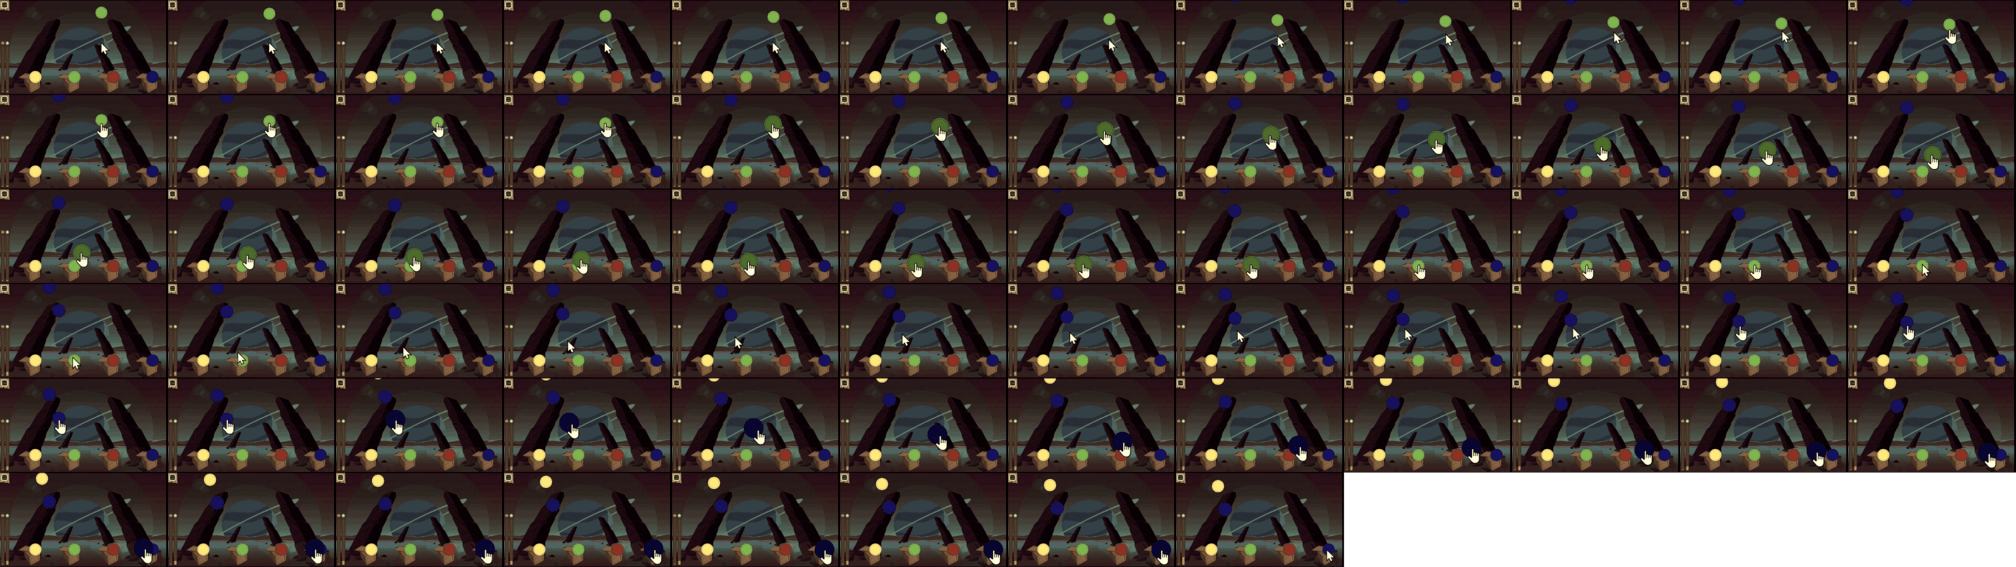
\includegraphics[width=1\textwidth]{figures/spreadsheet}
    \caption{Example: Spreadsheet}
    \label{fig:spreadsheet}
\end{figure}

\section{Concept of the Learning Environment}\label{sec:concept-of-the-learning-environment}
Through the given boundary conditions and requirements the environment is split into multiple parts/scenes.

\subsection{Drop Down Menu}\label{subsec:drop-down-menu}
Throughout the whole experience, the user can open a menu with a button.
This button is always visible.
Once the menu is open, the user may close the menu and return to the current scene,
exit the current scene and return to the level menu and go into fullscreen and back.
The current scene is paused while the menu is open as it can be distracting for the user,
if suddenly something pops up and covers parts of the visible and running scene.

\subsection{Welcome Screen}\label{subsec:welcome-screen}
The welcome screen is the starting point of the user experience.
Through this screen the user is greeted by showing the name of the game.
Through a click he may commence to the level menu.

\subsection{Level Menu}\label{subsec:level-menu}
In the level menu, the user is able to choose between different levels and games and can access the object summary.
Through the stars below each button the user can track his progress/score.
The progress can be resetted by the reset button.

\subsection{Object Summary}\label{subsec:object-summary}
The Object summary allows the user to get a feeling for all the different properties an object can have.
For that reason the number of objects per category is restricted to five, as there are over 1000 different objects.
Objects are draggable and sortable by each category with a click on a respective button.

\subsection{Sorting with one Category}\label{subsec:sorting-with-one-category}
Here the user has to sort the static objects with one category by the given category.
As the user should be able to experience all categories, they are split into different levels.
Each level represents a category.
For motivation, the user can track his progress.
The Progress is defined by objects sorted the right and the wrong way.

The amount of objects to sort, as well as the amount of properties of the category
is randomly selected each time you start the game.

\subsection{Sorting with one category under difficult conditions}\label{subsec:sorting-with-one-category-under-difficult-conditions}
Here the user has to sort falling objects with one category by the given category.
As the user should be able to experience all categories, they are split into different level.
Each level represents a category.
For motivation, the user can track his progress.
The progress is defined by objects missed, sorted the right and the wrong way.
To make the task harder, dummy objects are added.
Those objects look similar to the original ones but with a succinct characteristic.
There are no negative points for missing such an object but negative points for sorting them in any way.

For more diversity, the amount of falling objects to sort, as well as the amount of properties of the category
is randomly selected each time you start the game.

\subsection{Sorting with restricted space}\label{subsec:sorting-with-restricted-space}
In this scene the user has to sort a given number of objects with all properties shown into boxes with limited space.
The objects in one box must have at least one property in common and
can be put into the box and taken out an infinite amount of times.

To make the game more difficult, this level is split into two.
The first level has boxes with the size 6, 4, 2 and the second one boxes with the size 6, 5, 4.

\subsection{Object pairing - easy version}\label{subsec:object-pairing---easy-version}
In this game, twelve objects with three categories are shown.
the user has to select three objects which have to fulfil the following.
For each category (color, shape and number of holes/dots) one of the following conditions has to hold:
\begin{itemize}
    \item They must be the same (blue, blue, blue)
    \item They must be completely different (square, triangle, circle)
\end{itemize}

\begin{figure}[H]
    \centering
    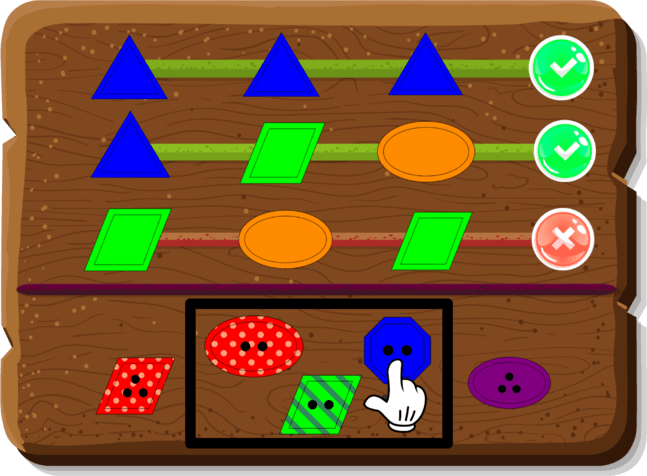
\includegraphics[width=0.8\textwidth]{figures/setexample}
    \caption{Example: Matching Set}
    \label{fig:setexample1}
\end{figure}

If the user needs help, there is a helper bar which can be accessed by a button with a question mark on it.
The helper bar shows which categories fulfil the conditions and which do not
by coloring the category symbols on the bar in green or red.

The game is time limited. The remaining time is shown by a bar.
If you select three objects which fulfil the conditions, more time will be added.
After a set amount of correct selected objects, the game will end.

If there are no three objects that fulfil the conditions, the playfield will be generated anew.

\subsection{Object pairing - normal version}\label{subsec:object-pairing---normal-version}
In this game, twelve objects with four categories are shown.
the user has to select three objects which have to fulfil the following.
For each category (color, filling, shape and number of holes/dots) one of the following conditions has to hold:
\begin{itemize}
    \item They must be the same (blue, blue, blue)
    \item They must be completely different (square, triangle, circle)
\end{itemize}

\begin{figure}[H]
    \centering
    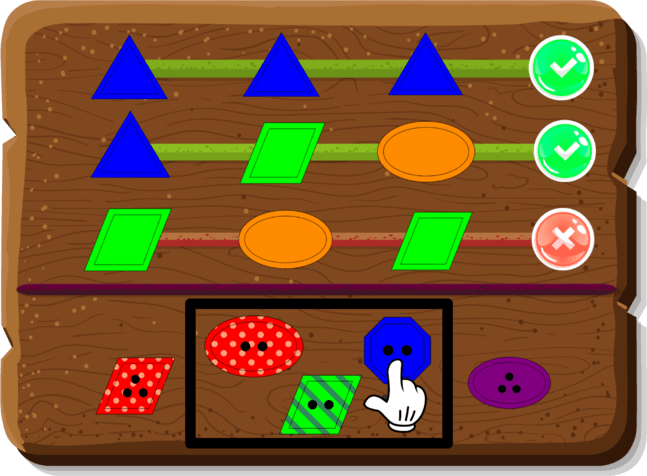
\includegraphics[width=0.8\textwidth]{figures/setexample}
    \caption{Example: Matching Set}
    \label{fig:setexample2}
\end{figure}

If the user needs help, there is a helper bar which can be accessed by a button with a question mark on it.
The helper bar shows which categories fulfil the conditions and which do not
by coloring the category symbols on the bar in green or red.

The game is time limited. The remaining time is shown by a bar.
If you select three objects which fulfil the conditions, more time will be added.
After a set amount of correct selected objects, the game will end.

If there are no three objects that fulfil the conditions, the playfield will be generated anew.

\subsection{Score Screen}\label{subsec:score-screen}
After a task has been completed, there is going to be a score.
This score is represented here with a displayed number of stars.
The minimum of starts is zero and the maximum is three.
If the user is unhappy with his results, he can replay the game by clicking on the replay button.

\subsection{Introduction}\label{subsec:introduction}
Before each game starts, a sample animation of the task beforehand is being shown.
The current scene is paused in the meantime, so that the user has enough time to find out what he has to do.

\section{Code structure of the learning environment}\label{sec:code-structure-of-the-learning-environment}
Our learning environment consists of different scenes each one inheriting the base scene.
The following subsections won't contain the whole code as some parts are trivial to understand.
Instead a summary of the scenes purpose and crucial parts are shown and explained.

The full code can be accessed in the appendix.

\begin{figure}[H]
    \centering
    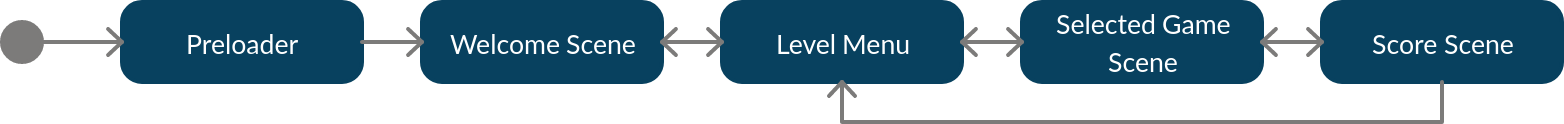
\includegraphics[width=1\textwidth]{figures/statediagram}
    \caption{Scene Statediagram}
    \label{fig:statediagram}
\end{figure}

\subsection{BaseScene}\label{subsec:basescene}
This scene contains methods and fields which are necessary in multiple scenes
(e.g. the scene transition, identifier of the scene, ...).

The transition is a mask in the form of a circle laid over a black rectangle.
Masks have to be applied to every object they have to mask.
So a simple solution was to lay a black rectangle over the whole scene and mask it.
The animated transition is created by increasing or decreasing the radius of the circle
mask according to the wanted animation (IN/OUT).

\begin{lstlisting}[style=TypeScript, caption={BaseScene.ts}]
    ...
    private transitionInit(): void {
        // Shape of the graphical transition
        const circle: Phaser.GameObjects.Graphics = this.add.graphics();

        // Shape of the screen
        const rectangle: Phaser.GameObjects.Rectangle = this.add.rectangle(0, 0, this.cameras.main.width, this.cameras.main.height, 0x000000);

        // Define circle as the mask
        const mask: Phaser.Display.Masks.GeometryMask = circle.createGeometryMask();

        circle.setPosition(this.cameras.main.width / 2, this.cameras.main.height / 2);
        circle.fillCircle(0, 0, 0.1);
        circle.setDepth(0);

        mask.setInvertAlpha(true);

        rectangle.setDepth(1);
        rectangle.setOrigin(0, 0);
        rectangle.setMask(mask);

        circle.fillCircle(0, 0, 0.1);

        this.transition = [circle, rectangle];
    }
\end{lstlisting}

\subsection{PreloadAssets}\label{subsec:preloadassets}
In the method "preload()" the files used later on can be loaded into the respective managers/cache.
If files are loaded in a method outside of the preload method, the loader has to be started manually (in the code).
Now every asset loaded this way has a unique identifier and can be used in future scene
as long as it is not removed explicitly.
The asset can as such be loaded into the managers/cache in every scene,
so that only the actual used assets are loaded.
The advantage of this is that you can save time and storage.
But the disadvantage is that you have to be connected to the internet the whole time.
Should the connection be severed for only a short time, objects might not be displayed correctly.
With a "preload" scene in the beginning all available assets are loaded,
so that after the longer loading time the game can run fluently,
without problems and most importantly without a connection to the internet.

The attributes and path of objects in the imported json file [REFERENCE TO EXPLANATION TOP]
can be accessed by filename.["fieldname"] or filename.fieldname:

\begin{lstlisting}[style=TypeScript, caption={Example json file access}]
    ...
    for (let category of loadedJsonObjectFile['categories']) {
        console.log("URL: " + category['url']);
        console.log("Name: " + category['validElements']['name']);
        console.log("ValidElement urls: " + category['validElements']['urls']);
    }

    for (let image of loadedJsonObjectFile['images']) {
        console.log("Name: " + image.name);
        console.log("Cat1: " + image.cat1);
        ...
    }
    ...
\end{lstlisting}

The way the objects files are preloaded into the respective managers is shown below.

\begin{lstlisting}[style=TypeScript, caption={preloadAsset.ts}]
    ...
    private preload(): void {
        this.load.setPath('assets/geometrical_objects/');
        this.load.json('objects', 'geometrical_objects.json');
        ...
    }
    ...
    private preLoadImages(): void {
        // Load category and object images
        const jsonObject: any = this.cache.json.get('objects');

        for (let category of jsonObject['categories']) {
            this.load.setPath('assets/geometrical_objects/categories/');
            this.load.image(category['name'], category['url']);

            this.load.setPath('assets/geometrical_objects/images/');
            for (let property of category['validElements']) {
                for (let url of property['urls']) {
                    this.load.image(url, url);
                }
            }
        }

        for (let image of jsonObject['images']) {
            this.load.image(image['name'], image['name']);
        }
        ...
    }
    ...
\end{lstlisting}

\subsubsection{Image Game Objects}
Instead of representing an image as a normal image in game, sprites, a special texture, is used.
A sprite game object can display both static and animated images in your game.
They have input events, additional functions, fields and physics bodies.
The main difference between a sprite and an image game object is that you cannot animate images.

\subsection{DropDownMenu}\label{subsec:dropdownmenu}
In this scene the drop down menu is created.
This scene is never stopped and is always on top of other scenes.

The following code in every other scene ensures this:
\begin{lstlisting}[style=TypeScript, caption={Send current scene to back}]
    ...
    create(): void {
        this.game.scene.sendToBack(this.getKey());
        ...
    }
    ...
\end{lstlisting}

As the drop down animation takes time, it was necessary to create a boolean field as a lock.
This ensures that the closing and opening animation won't interfere with each other.
The lock is freed after the completion of an event/animation.

\begin{lstlisting}[style=TypeScript, caption={Lock aquiring and freeing}]
    ...
    if (!this.lock) {
        this.lock = true;
        ...
    }
    ...
    onComplete: () => this.lock = false;
    ...
\end{lstlisting}

While the menu is down/open, the current scene has to be paused.
This is achieved by accessing the other scene by fetching the key of the only other active scene and pausing it.
Important to note is, that the last started/activated scene is at position 0 in the array of all active scenes.
\begin{lstlisting}[style=TypeScript, caption={Fetching current active scene}]
    ...
    const key_paused_scene: string = this.game.scene.getScenes(true)[0].key;
    this.game.scene.pause(key_paused_scene);
    this.key_paused_scene = key_paused_scene;
    ...
\end{lstlisting}

The same trick is used for closing all current scenes when exiting (without the dropDownMenu Scene).

\subsection{WelcomeScene}\label{subsec:welcomescene}
A blinking finger is added to the screen so that the user knows that he can advance by clicking on the screen.

\subsection{LevelMenuSceneScene}\label{subsec:levelmenuscenescene}
Levels with the same difficulty are distinguished by numbers from one to four.
Levels with another difficulty are distinguished by images of monsters with different level of spookiness.

\begin{figure}[H]
    \centering
    
\includegraphics[width=0.2\textwidth]{figures/easylevelicon}
    \caption{Easy Level Icon}
    \label{fig:easylevelicon}
\end{figure}

\begin{figure}[H]
    \centering
    
\includegraphics[width=0.2\textwidth]{figures/mediumlevelicon}
    \caption{Medium Level Icon}
    \label{fig:mediumlevelicon}
\end{figure}

\begin{figure}[H]
    \centering
    
\includegraphics[width=0.2\textwidth]{figures/hardlevelicon}
    \caption{Hard Level Icon}
    \label{fig:hardlevelicon}
\end{figure}

\subsection{IntroScene}\label{subsec:introscene}
To pause the current scene and still play the introduction animation, a separate scene is necessary.
Each time an intro has to be played, the intro scene is started anew.
The current scene is pauses itself when the intro scene is started and the name/key/identifier
of the paused scene is given to the intro scene.
That way the intro scene can resume the paused scene and then stop itself.

The respective intro material is selected via the name/key/identifier of the paused scene.

\subsection{SortingScene}\label{subsec:sortingscene}
To sort the displayed objects by their respective subcategory by clicking on one of the category buttons,
random coordinates are needed dependant on the screen size and object size.
\begin{lstlisting}[style=TypeScript, caption={returnQuad() (sortingScene.ts)}]
    ...
    private returnQuad(quadrant: number, quadrantType: number): number[] {
        let ret: number[] = null;
        ...
        const leftOffsite: number = 100;
        const rightOffsite: number = 0;
        const topOffsite: number = 0;
        const bottomOffsite: number = 100;

        // Has entries dependant of
        const horizontal: number[] = [];

        // Has numberOfLines + 1 entries
        const vertical: number[] = [];

        horizontal.push(leftOffsite);

        vertical.push(topOffsite);

        switch (quadrantType) {
            case 3: {
                horizontal.push(leftOffsite + (this.cameras.main.width - leftOffsite - rightOffsite) / 3);
                horizontal.push(leftOffsite + (this.cameras.main.width - leftOffsite - rightOffsite) * 2 / 3);
                break;
            }
            case 4: {
                horizontal.push(leftOffsite + (this.cameras.main.width - leftOffsite - rightOffsite) / 2);
                vertical.push(topOffsite + (this.cameras.main.height - topOffsite - bottomOffsite) / 2);
                break;
            }
            case 6: {
                horizontal.push(leftOffsite + (this.cameras.main.width - leftOffsite - rightOffsite) / 3);
                horizontal.push(leftOffsite + (this.cameras.main.width - leftOffsite - rightOffsite) * 2 / 3);
                vertical.push(topOffsite + (this.cameras.main.height - topOffsite - bottomOffsite) / 2);
                break;
            }
            default: {
                break;
            }
        }

        horizontal.push(this.cameras.main.width - rightOffsite);
        vertical.push(this.cameras.main.height - bottomOffsite);

        switch (quadrantType) {
            case 3: {
                ret = [Phaser.Math.RND.between(horizontal[quadrant] + spriteSizeHalf, horizontal[quadrant + 1] - spriteSizeHalf), Phaser.Math.RND.between(vertical[0] + spriteSizeHalf + this.cameras.main.height / 8, vertical[1] - spriteSizeHalf - this.cameras.main.height / 8)];
                break;
            }
            case 4: {
                if (quadrant < 2) {
                    ret = [Phaser.Math.RND.between(horizontal[quadrant] + spriteSizeHalf, horizontal[quadrant + 1] - spriteSizeHalf), Phaser.Math.RND.between(vertical[0] + spriteSizeHalf, vertical[1] - spriteSizeHalf)];
                } else {
                    ret = [Phaser.Math.RND.between(horizontal[quadrant \% 2] + spriteSizeHalf, horizontal[(quadrant \% 2) + 1] - spriteSizeHalf), Phaser.Math.RND.between(vertical[1] + spriteSizeHalf, vertical[2] - spriteSizeHalf)];

                }
                break;
            }
            case 6: {
                if (quadrant < 3) {
                    ret = [Phaser.Math.RND.between(horizontal[quadrant] + spriteSizeHalf, horizontal[quadrant + 1] - spriteSizeHalf), Phaser.Math.RND.between(vertical[0] + spriteSizeHalf, vertical[1] - spriteSizeHalf)];
                } else {
                    ret = [Phaser.Math.RND.between(horizontal[quadrant \% 3] + spriteSizeHalf, horizontal[(quadrant \% 3) + 1] - spriteSizeHalf), Phaser.Math.RND.between(vertical[1] + spriteSizeHalf, vertical[2] - spriteSizeHalf)];
                }
                break;
            }
            default: {
                break;
            }
        }
        return ret;
    }
\end{lstlisting}

\subsection{PropertySortingScene}\label{subsec:propertysortingscene}
To specify the difficulty level, two fields are needed:
\begin{lstlisting}[style=TypeScript, caption={Level fields (propertySortingScene.ts)}]
    ...
    private setCat: number;
    ...
    private infinite: boolean;
    ...
\end{lstlisting}

In contrast to other scenes, objects must have the type Phaser.Physics.Arcade.Sprite as only arcade sprites have the
possibility of an acceleration in a direction.

As additional visual feature objects get a random spin velocity and the time a object spawns gets shorter over time.

\subsection{RestrictedSortingScene}\label{subsec:restrictedsortingscene}
To check if objects in the same box have some property in common,
the four properties of a object are taken as a list of strings and intersected with the other list of strings from other
objects in the same box.
If finally there is no empty list, the objects have some property in common and thus this is a valid solution for one box.
Which one does not matter to us in this case.
In this way, it is possible that there are multiple solutions which were not intended but also correct.

\begin{lstlisting}[style=TypeScript, caption={equalityCheck (restrictedSortingScene.ts)}]
    ...
        private equalityCheck(gameObject: Phaser.GameObjects.Sprite, dropZone: Phaser.GameObjects.Zone): boolean {
        ...
        let mergeArray: any[] = [];
        ...
        for (let cat of this.jsonObject['categories']) {
            mergeArray = [...mergeArray, ...cat['validElements']];
        }
        mergeArray.forEach((element, index, array) => array[index] = element.name);
        ...
        [...this.objZoneMap.filter((element, index) => this.zoneObjMap[index].name === dropZone.name), gameObject].forEach(function (element) {
            mergeArray = mergeArray.filter((x) => element.getData('properties').includes(x));
        });
        ...
        return (mergeArray.length > 0);
    }
    ...
\end{lstlisting}

\subsection{GameScene}\label{subsec:gamescene}
In the game scene three marked objects are checked for equality
if the checker was not already run for those three objects.

\begin{lstlisting}[style=TypeScript, caption={update (gameScene.ts)}]
    update(time: number): void {
        ...
        if (!this.checked && this.arrayMarked.getLength() >= 3) {
            this.checked = true;
            ...
        }
        ...
        if (timedata <= 0) {
            this.checked = true;

            ...
        } else {
            timedata -= this.timedataStepsize;
            this.timefluid.setData('timeY', timedata);
            this.timefluid.setScale(this.timefluid.getData('timeX'), timedata);
        }
    }
\end{lstlisting}

As 'gameMax' is calculated with a quotient there is a rounding error in the floating point arithmetic.
To even this error we add or subtract epsilon, the maximum relative error of the rounding procedure.

\begin{lstlisting}[style=TypeScript, caption={updateProgressbar (gameScene.ts)}]
    ...
    if (this.points >= this.gamefluid.getData('gameMax') - Phaser.Math.EPSILON) {
        ...
    }
\end{lstlisting}

To mark the helpers menu icons the checkEquality method is modified
with a boolean to mark the icons while executing the check.

\begin{lstlisting}[style=TypeScript, caption={checkEquality (gameScene.ts)}]
    ...
    private checkEquality(sprite1: Phaser.GameObjects.GameObject, sprite2: Phaser.GameObjects.GameObject, sprite3: Phaser.GameObjects.GameObject, inGame: boolean): boolean {
        if (sprite1 instanceof Phaser.GameObjects.Sprite &&
            sprite2 instanceof Phaser.GameObjects.Sprite &&
            sprite3 instanceof Phaser.GameObjects.Sprite
        ) {
            // Return value
            let replaceObjects: boolean = true;

            for (let categoryIndicator of this.arrayCategory.getChildren()) {

                // Make sure your objects are sprites
                if (categoryIndicator instanceof Phaser.GameObjects.Sprite) {

                    // Clear tint
                    categoryIndicator.clearTint();

                    if (
                        sprite1.getData(categoryIndicator.name) === sprite2.getData(categoryIndicator.name) &&
                        sprite2.getData(categoryIndicator.name) === sprite3.getData(categoryIndicator.name) &&
                        sprite1.getData(categoryIndicator.name) === sprite3.getData(categoryIndicator.name)
                    ) {
                        if (inGame) {
                            categoryIndicator.setTintFill(0x00dd00);
                        }
                    } else if (
                        !(sprite1.getData(categoryIndicator.name) === sprite2.getData(categoryIndicator.name)) &&
                        !(sprite2.getData(categoryIndicator.name) === sprite3.getData(categoryIndicator.name)) &&
                        !(sprite1.getData(categoryIndicator.name) === sprite3.getData(categoryIndicator.name))
                    ) {
                        if (inGame) {
                            categoryIndicator.setTintFill(0x00dd00);
                        }
                    } else {
                        if (replaceObjects) {
                            replaceObjects = false;
                        }
                        if (inGame) {
                            // Mark category as red
                            categoryIndicator.setTintFill(0xdd0000);
                        }
                    }
                }
            }
            return replaceObjects;
        }
    }
\end{lstlisting}

To add another small gamification element in the form of a mini reward to the game, every time the user finds a matching
pair, some additional is added to the timer. So the user is even more motivated find pairs even faster.

\begin{lstlisting}[style=TypeScript, caption={updateProgressbar (gameScene.ts)}]
    ...
    let timedata: number = this.timefluid.getData('timeY');
    timedata += this.timedataStepsize * 5000;
    if (timedata > this.timefluid.getData('timeYMax')) {
        timedata = this.timefluid.getData('timeYMax');
    }
    ...
\end{lstlisting}

As frustrating as it is to find no matching pair,
it is ensured that there is at least one possible pair every time a new object is added.

\begin{lstlisting}[style=TypeScript, caption={INSERT (gameScene.ts)}]
    ...
    private rebuildDisplayedObjects(): void {
        ...
        for (let card of this.arrayDisplayed.getChildren()) {
            if (card instanceof Phaser.GameObjects.Sprite) {
                card.setVisible(false);
                this.arrayStack.add(card);
            }
        }

        this.arrayDisplayed.clear(false, false);

        this.initObjects();
    }
    ...
\end{lstlisting}

\subsection{ScoreScene}\label{subsec:scorescene}
The most important and special part in the score scene is the way the score is saved,
as explained in this \hyperref[ref:scorestorage]{section}.

\section{Final Look of the Learning Environment}\label{sec:final-look-of-the-learning-environment}
This section contains the final look of the learning environment.

\begin{figure}[H]
    \centering
    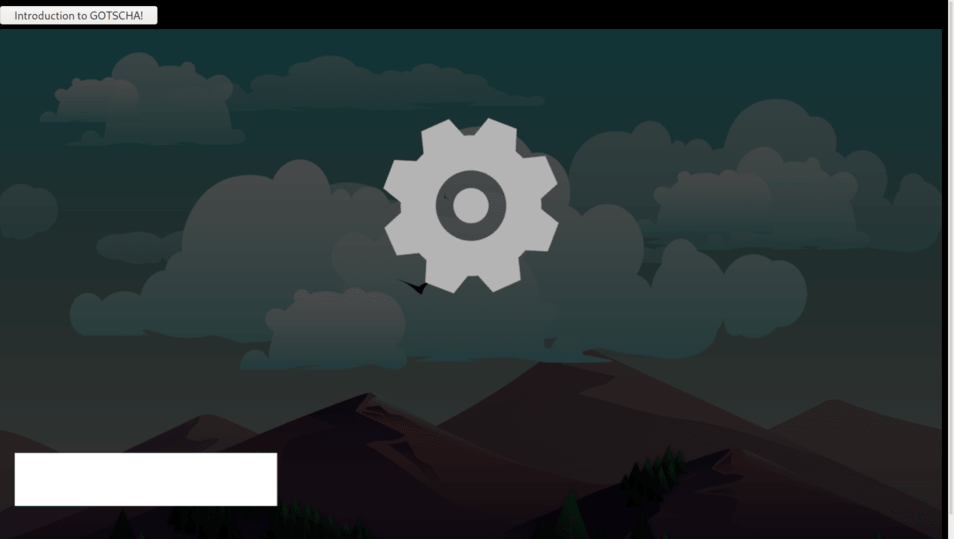
\includegraphics[width=1\textwidth]{figures/loadingscreen}
    \caption{Loading Screen}
    \label{fig:loadingscreen}
\end{figure}

\begin{figure}[H]
    \centering
    
\includegraphics[width=1\textwidth]{figures/welcomescreen}
    \caption{Title Screen}
    \label{fig:titlescreen}
\end{figure}

\begin{figure}[H]
    \centering
    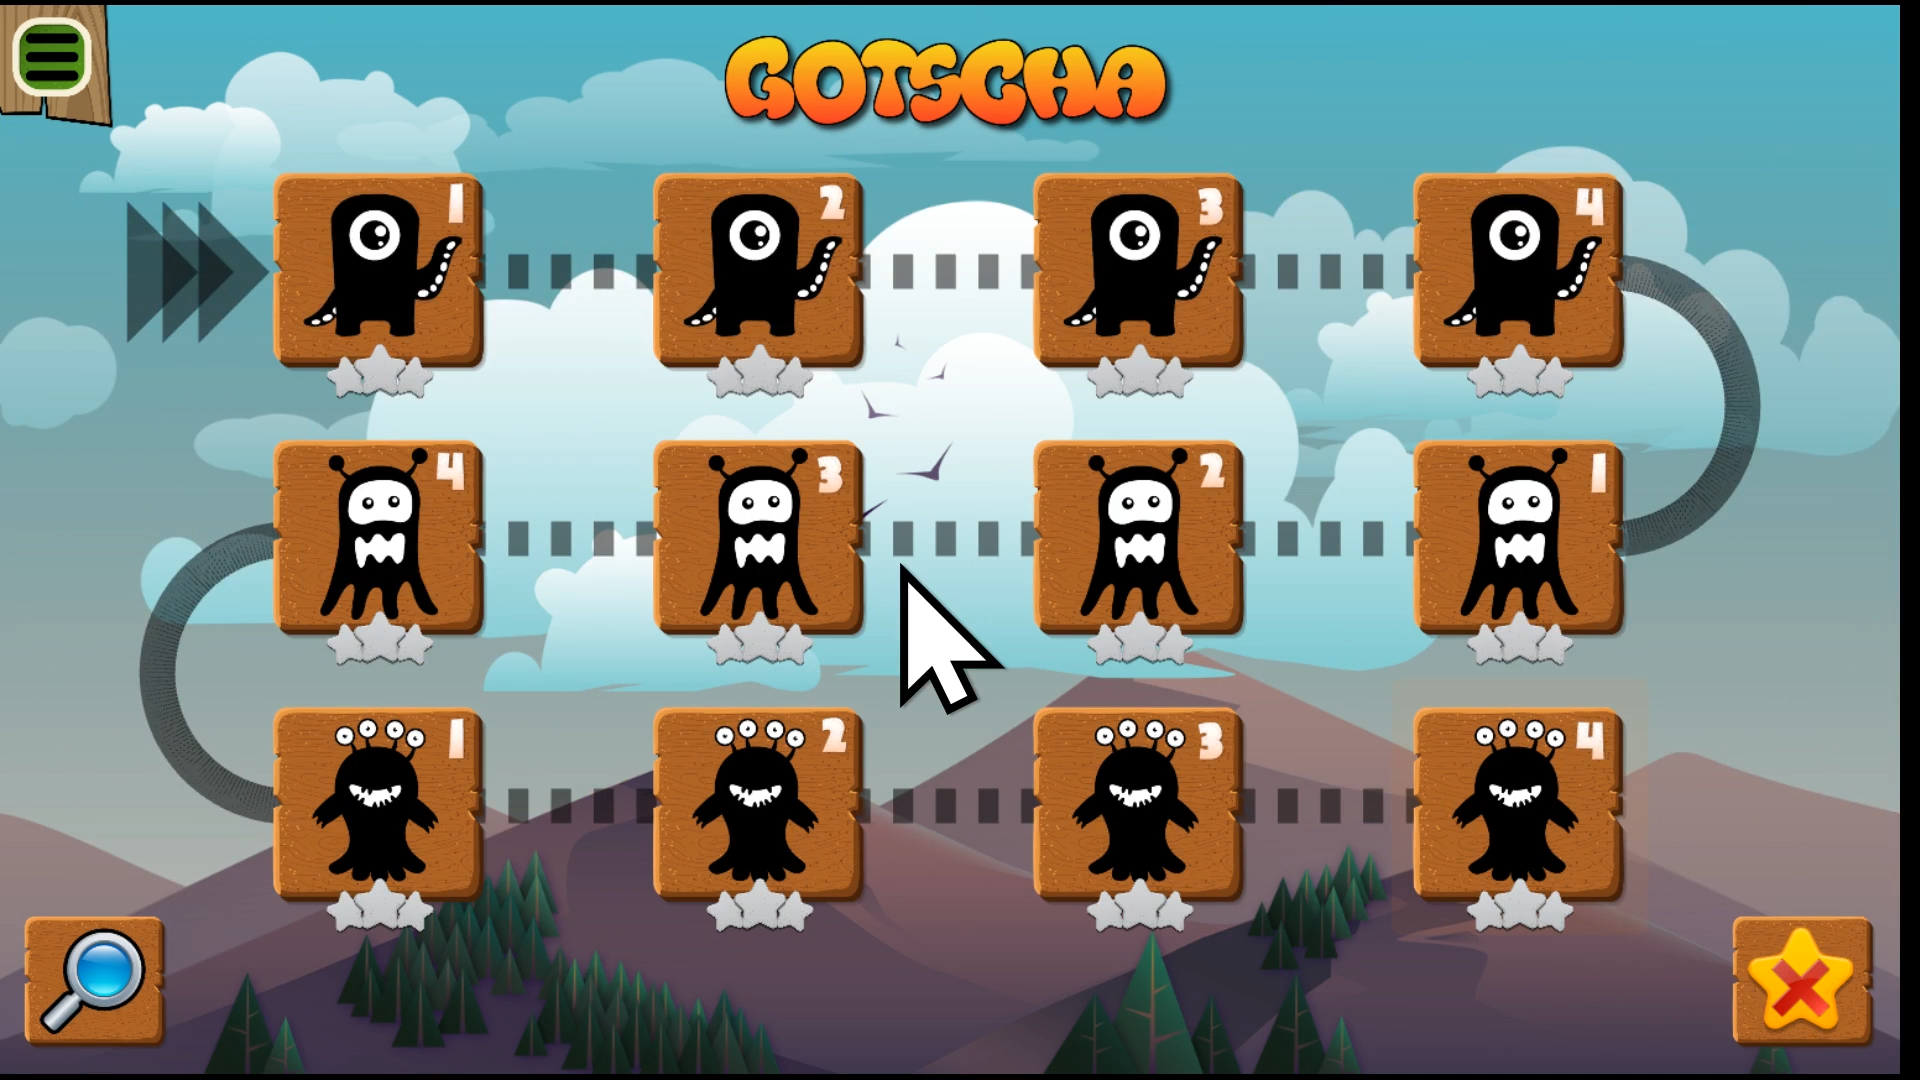
\includegraphics[width=1\textwidth]{figures/levelmenu}
    \caption{Level Menu}
    \label{fig:levelmenu}
\end{figure}

\begin{figure}[H]
    \centering
    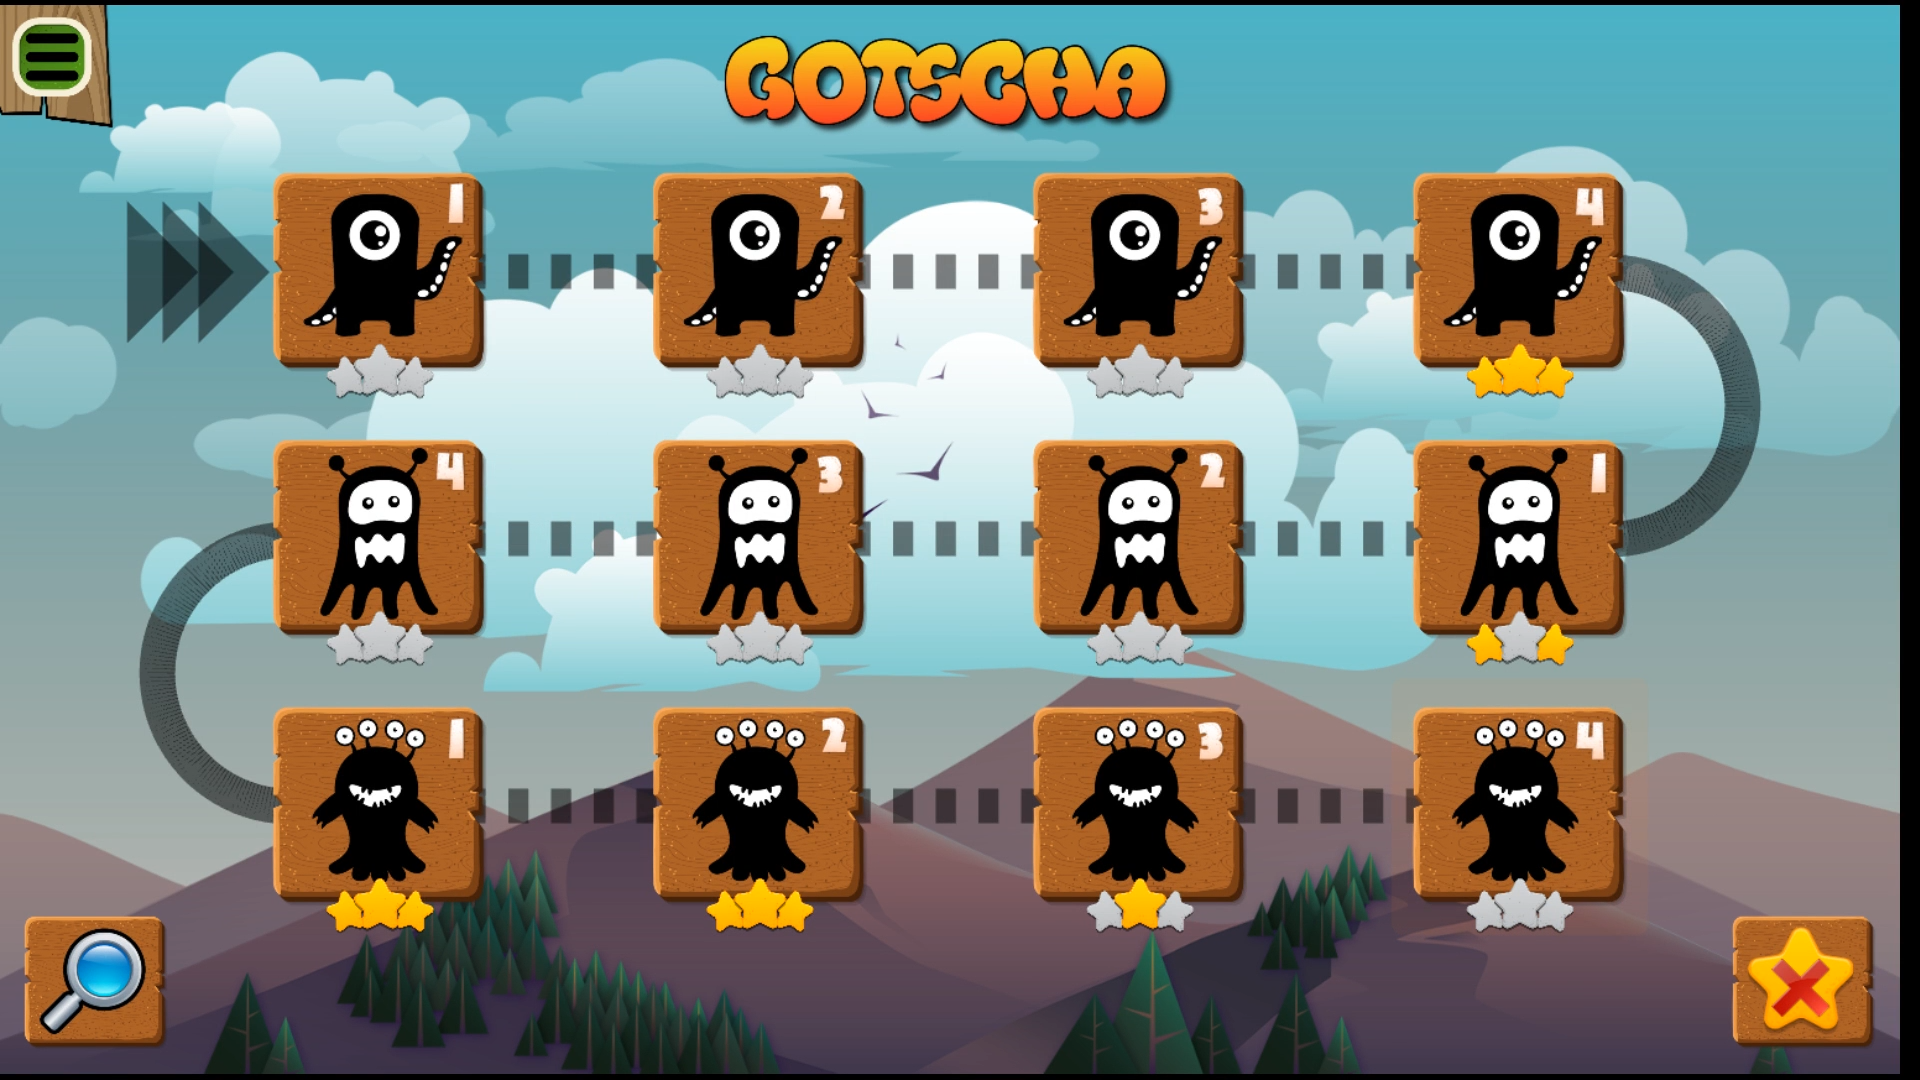
\includegraphics[width=1\textwidth]{figures/levelmenustars}
    \caption{Level Menu showing Stars}
    \label{fig:levelmenustars}
\end{figure}

\begin{figure}[H]
    \centering
    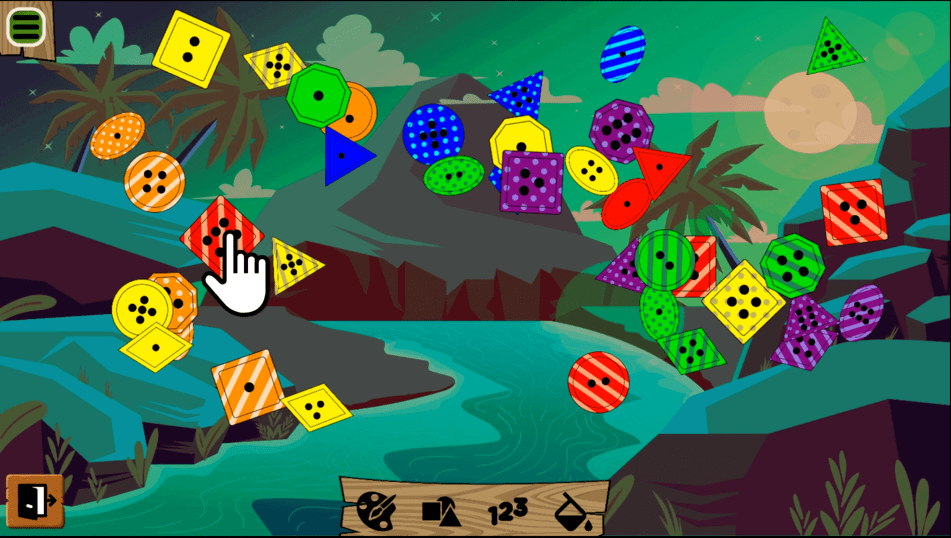
\includegraphics[width=1\textwidth]{figures/sortingscene1}
    \caption{Sorting Scene Category Mixture}
    \label{fig:sortingscene1}
\end{figure}

\begin{figure}[H]
    \centering
    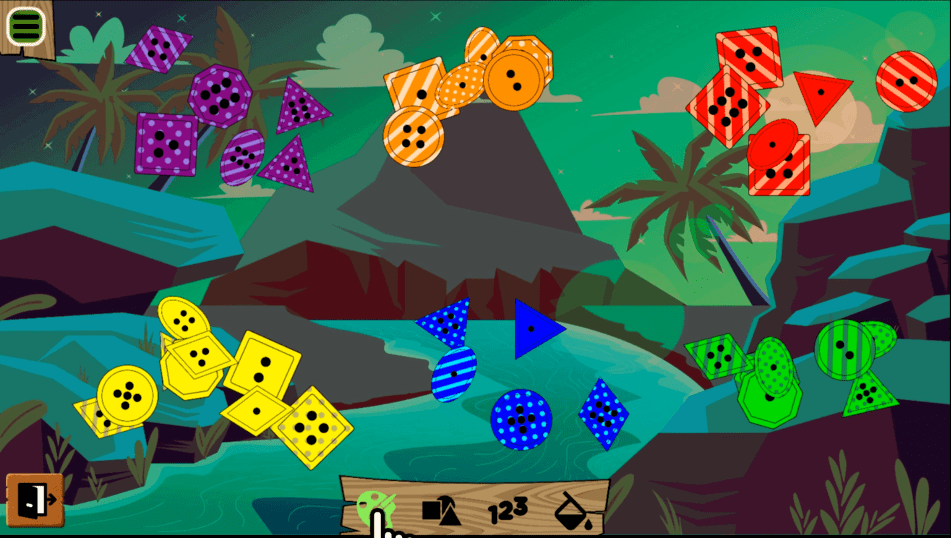
\includegraphics[width=1\textwidth]{figures/sortingscene2}
    \caption{Sorting Scene Category 1}
    \label{fig:sortingscene2}
\end{figure}

\begin{figure}[H]
    \centering
    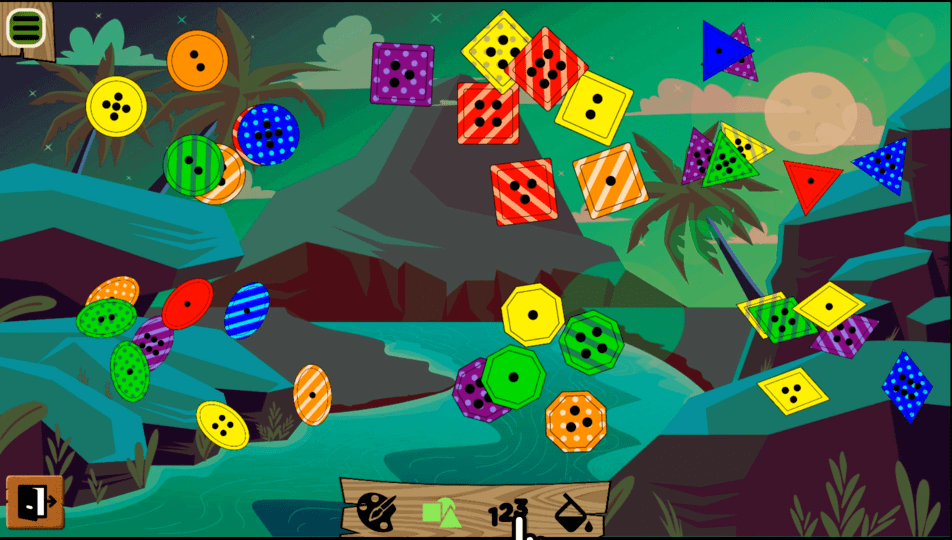
\includegraphics[width=1\textwidth]{figures/sortingscene3}
    \caption{Sorting Scene Category 2}
    \label{fig:sortingscene3}
\end{figure}

\begin{figure}[H]
    \centering
    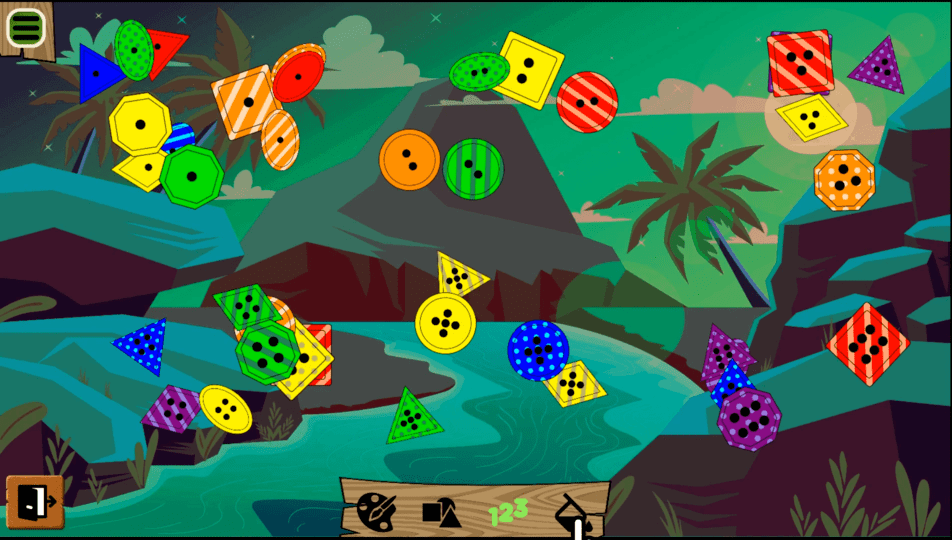
\includegraphics[width=1\textwidth]{figures/sortingscene4}
    \caption{Sorting Scene Category 3}
    \label{fig:sortingscene4}
\end{figure}

\begin{figure}[H]
    \centering
    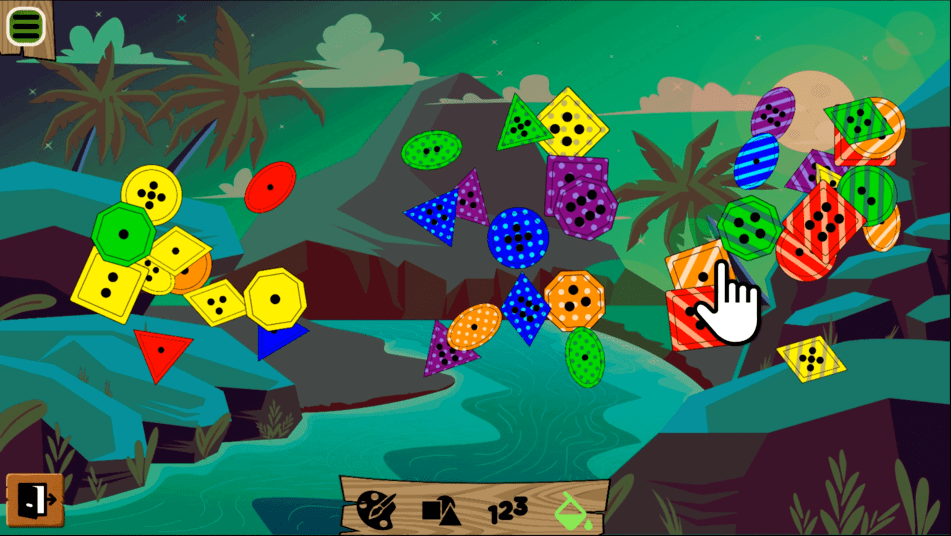
\includegraphics[width=1\textwidth]{figures/sortingscene5}
    \caption{Sorting Scene Category 4}
    \label{fig:sortingscene5}
\end{figure}

\begin{figure}[H]
    \centering
    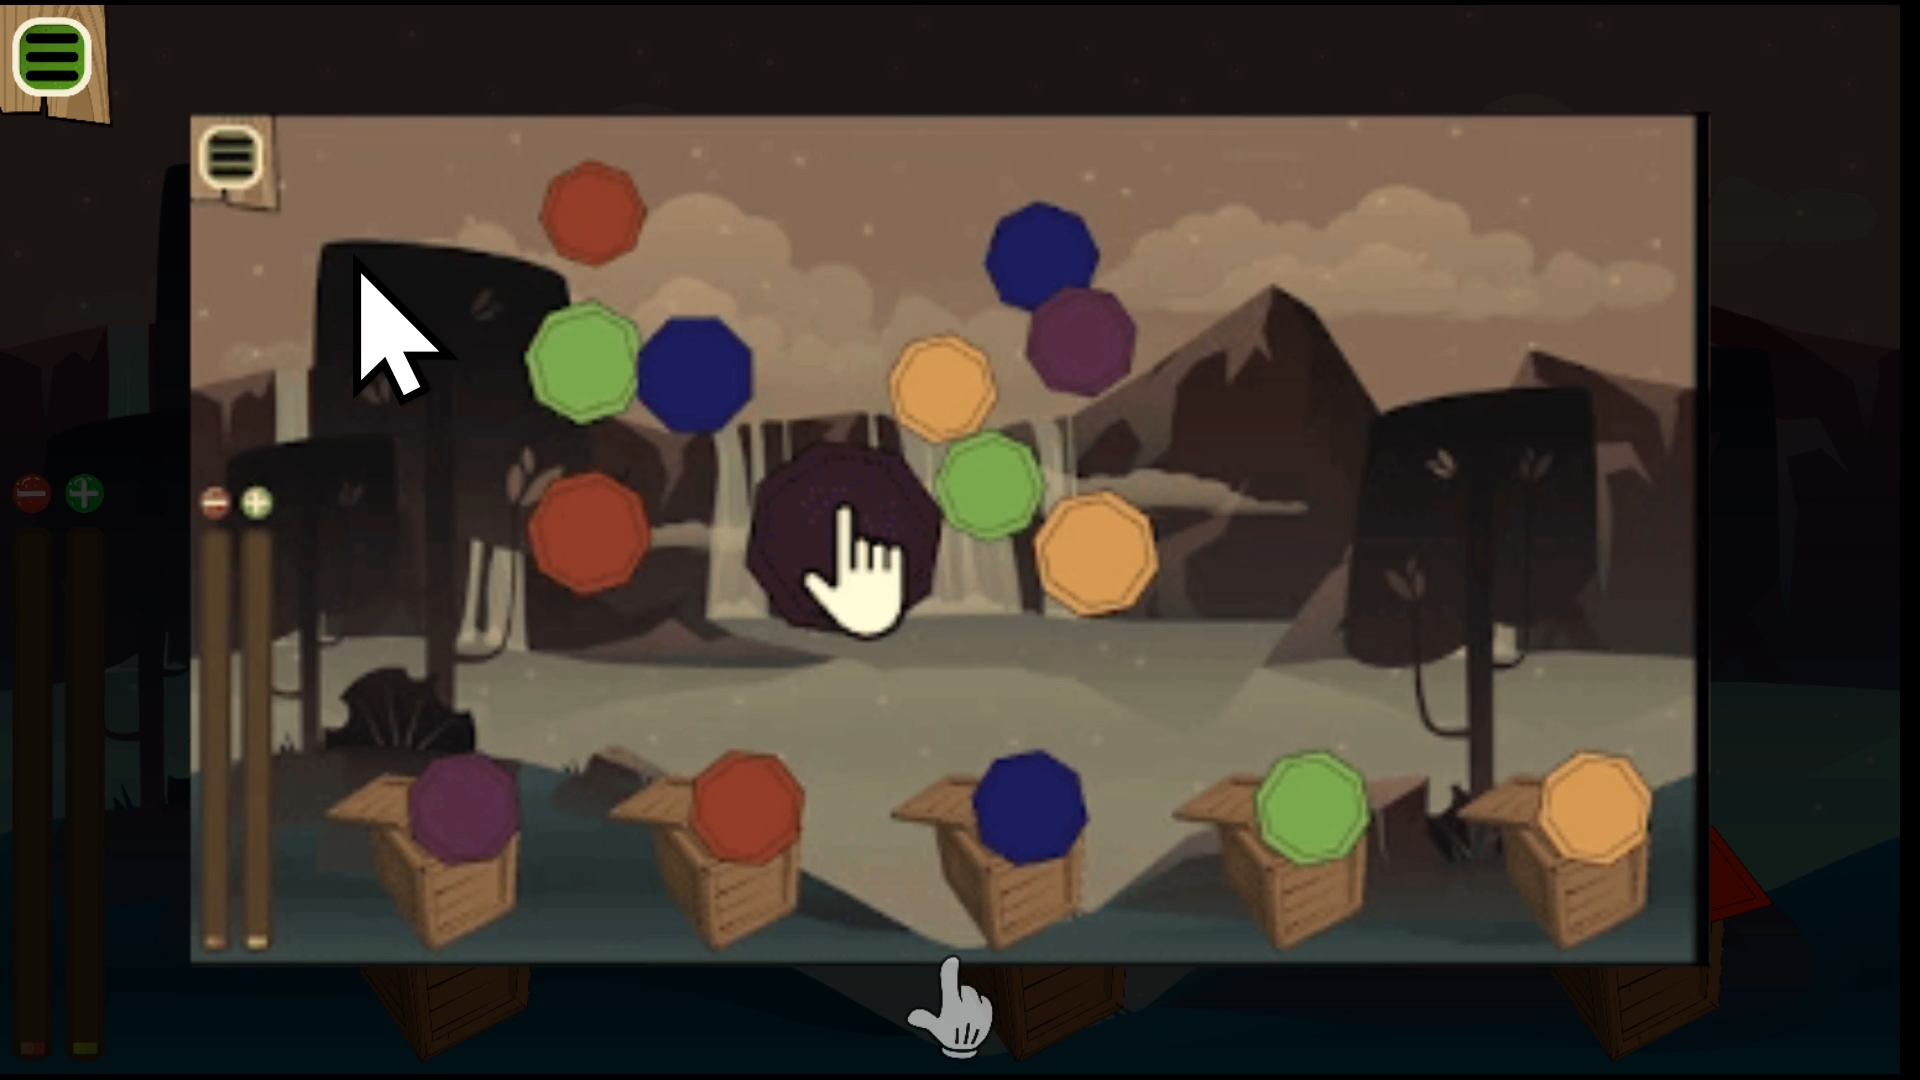
\includegraphics[width=1\textwidth]{figures/introduction}
    \caption{Introduction Screen to Sorting Scene}
    \label{fig:introduction}
\end{figure}

\begin{figure}[H]
    \centering
    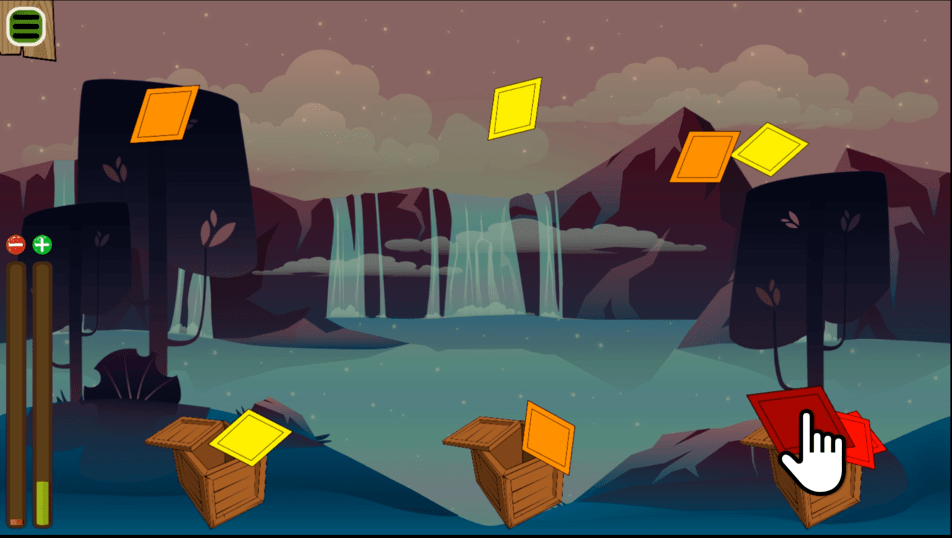
\includegraphics[width=1\textwidth]{figures/property1}
    \caption{Property Sorting Category 1}
    \label{fig:property1}
\end{figure}

\begin{figure}[H]
    \centering
    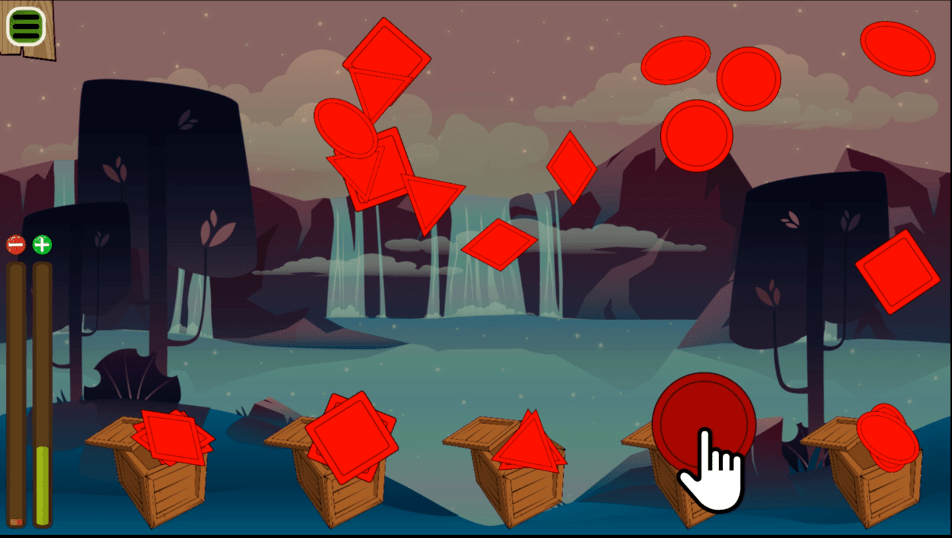
\includegraphics[width=1\textwidth]{figures/property2}
    \caption{Property Sorting Category 2}
    \label{fig:property2}
\end{figure}

\begin{figure}[H]
    \centering
    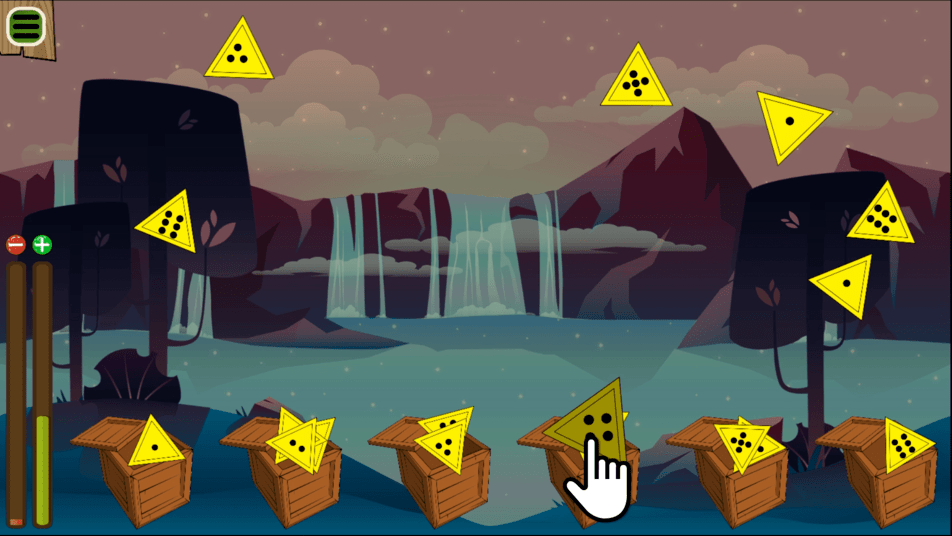
\includegraphics[width=1\textwidth]{figures/property3}
    \caption{Property Sorting Category 3}
    \label{fig:property3}
\end{figure}

\begin{figure}[H]
    \centering
    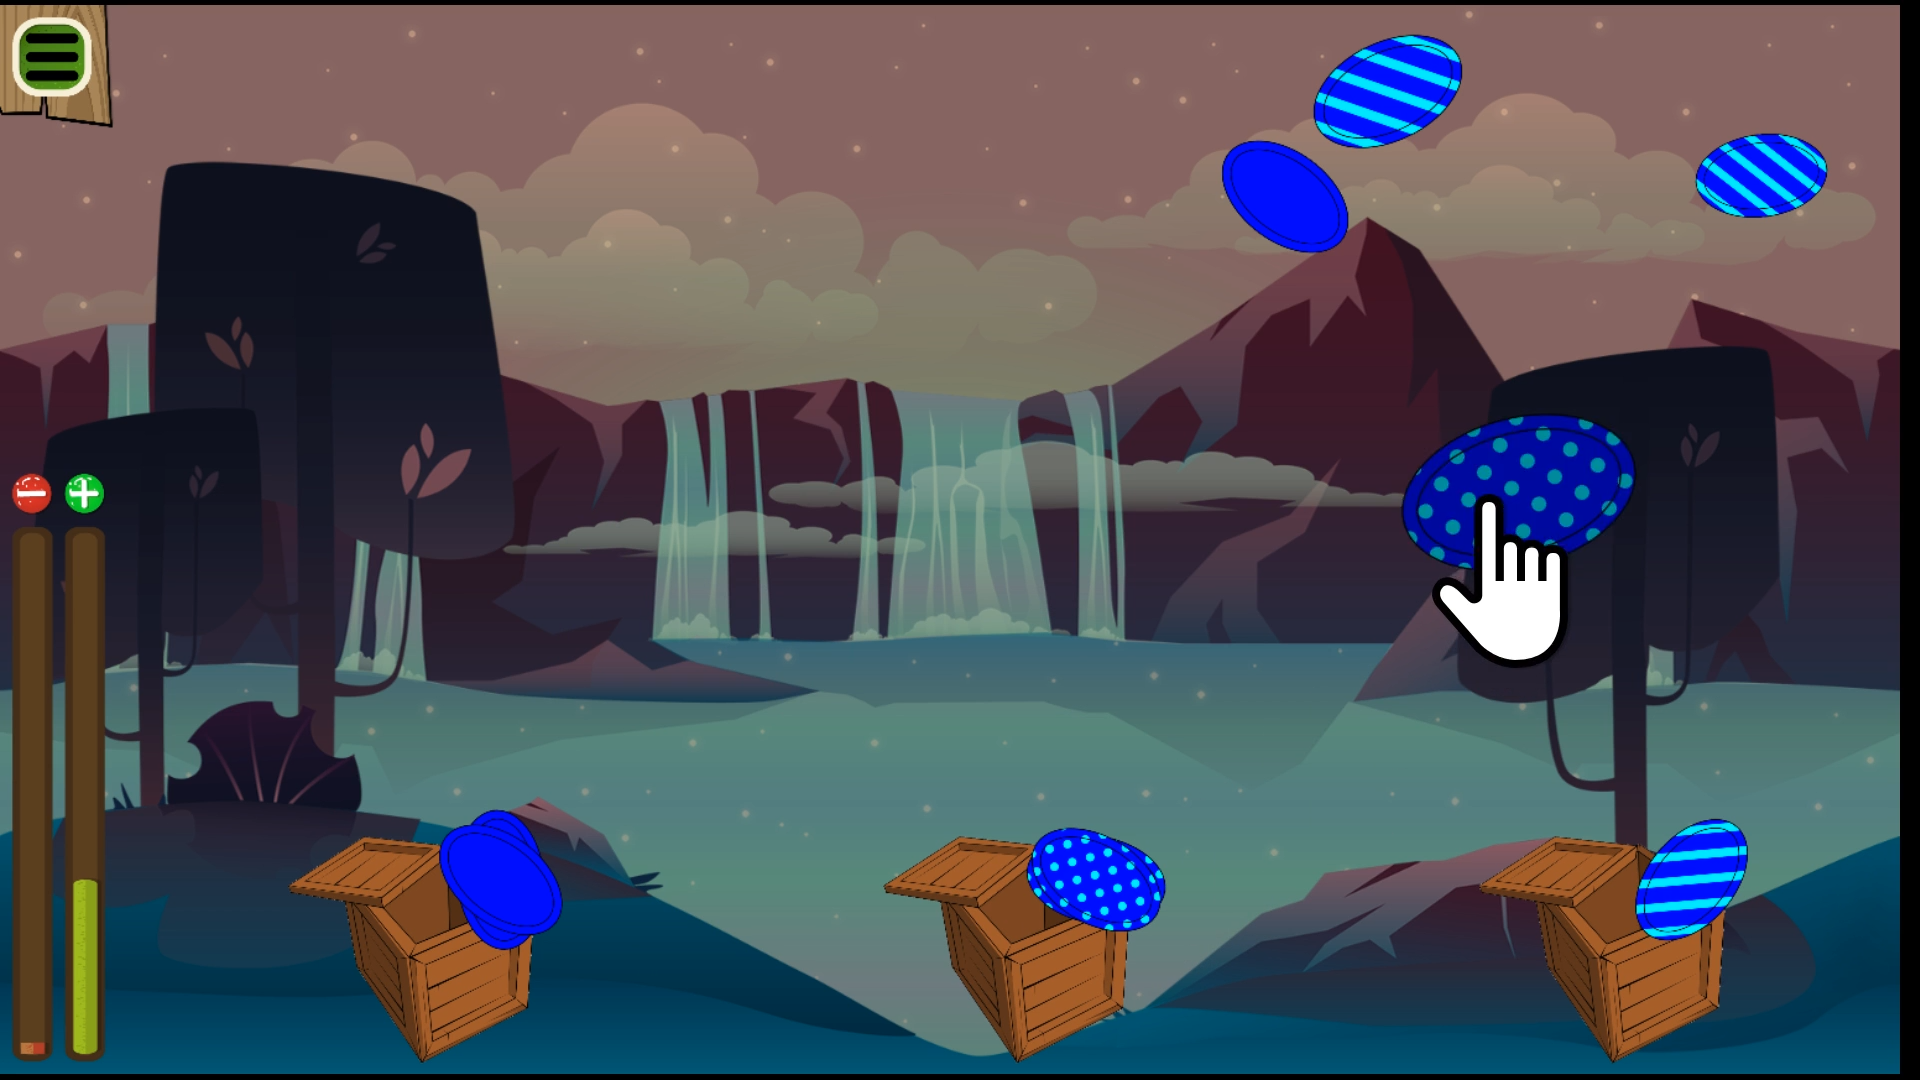
\includegraphics[width=1\textwidth]{figures/property4}
    \caption{Property Sorting Category 4}
    \label{fig:property4}
\end{figure}

\begin{figure}[H]
    \centering
    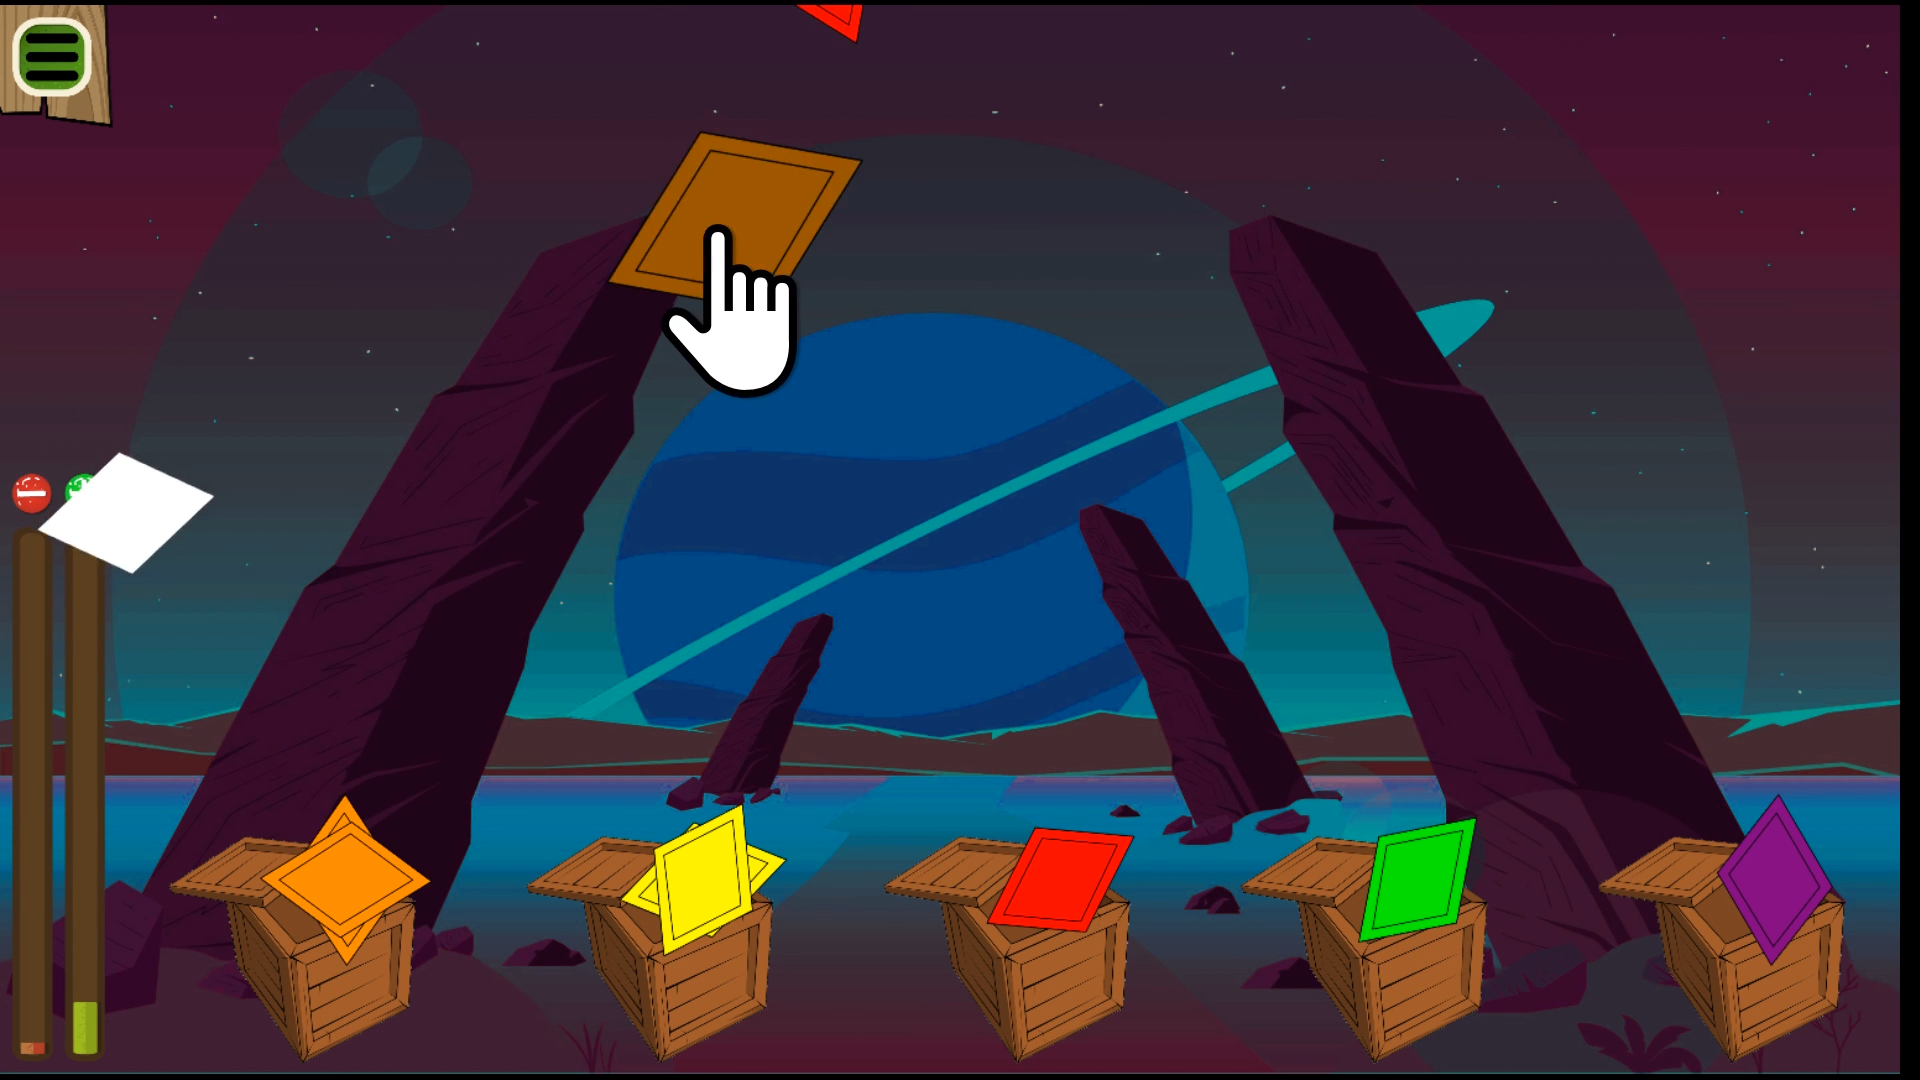
\includegraphics[width=1\textwidth]{figures/falling}
    \caption{Falling Property Sorting Category 1, 2-4 will be omitted}
    \label{fig:falling}
\end{figure}

\begin{figure}[H]
    \centering
    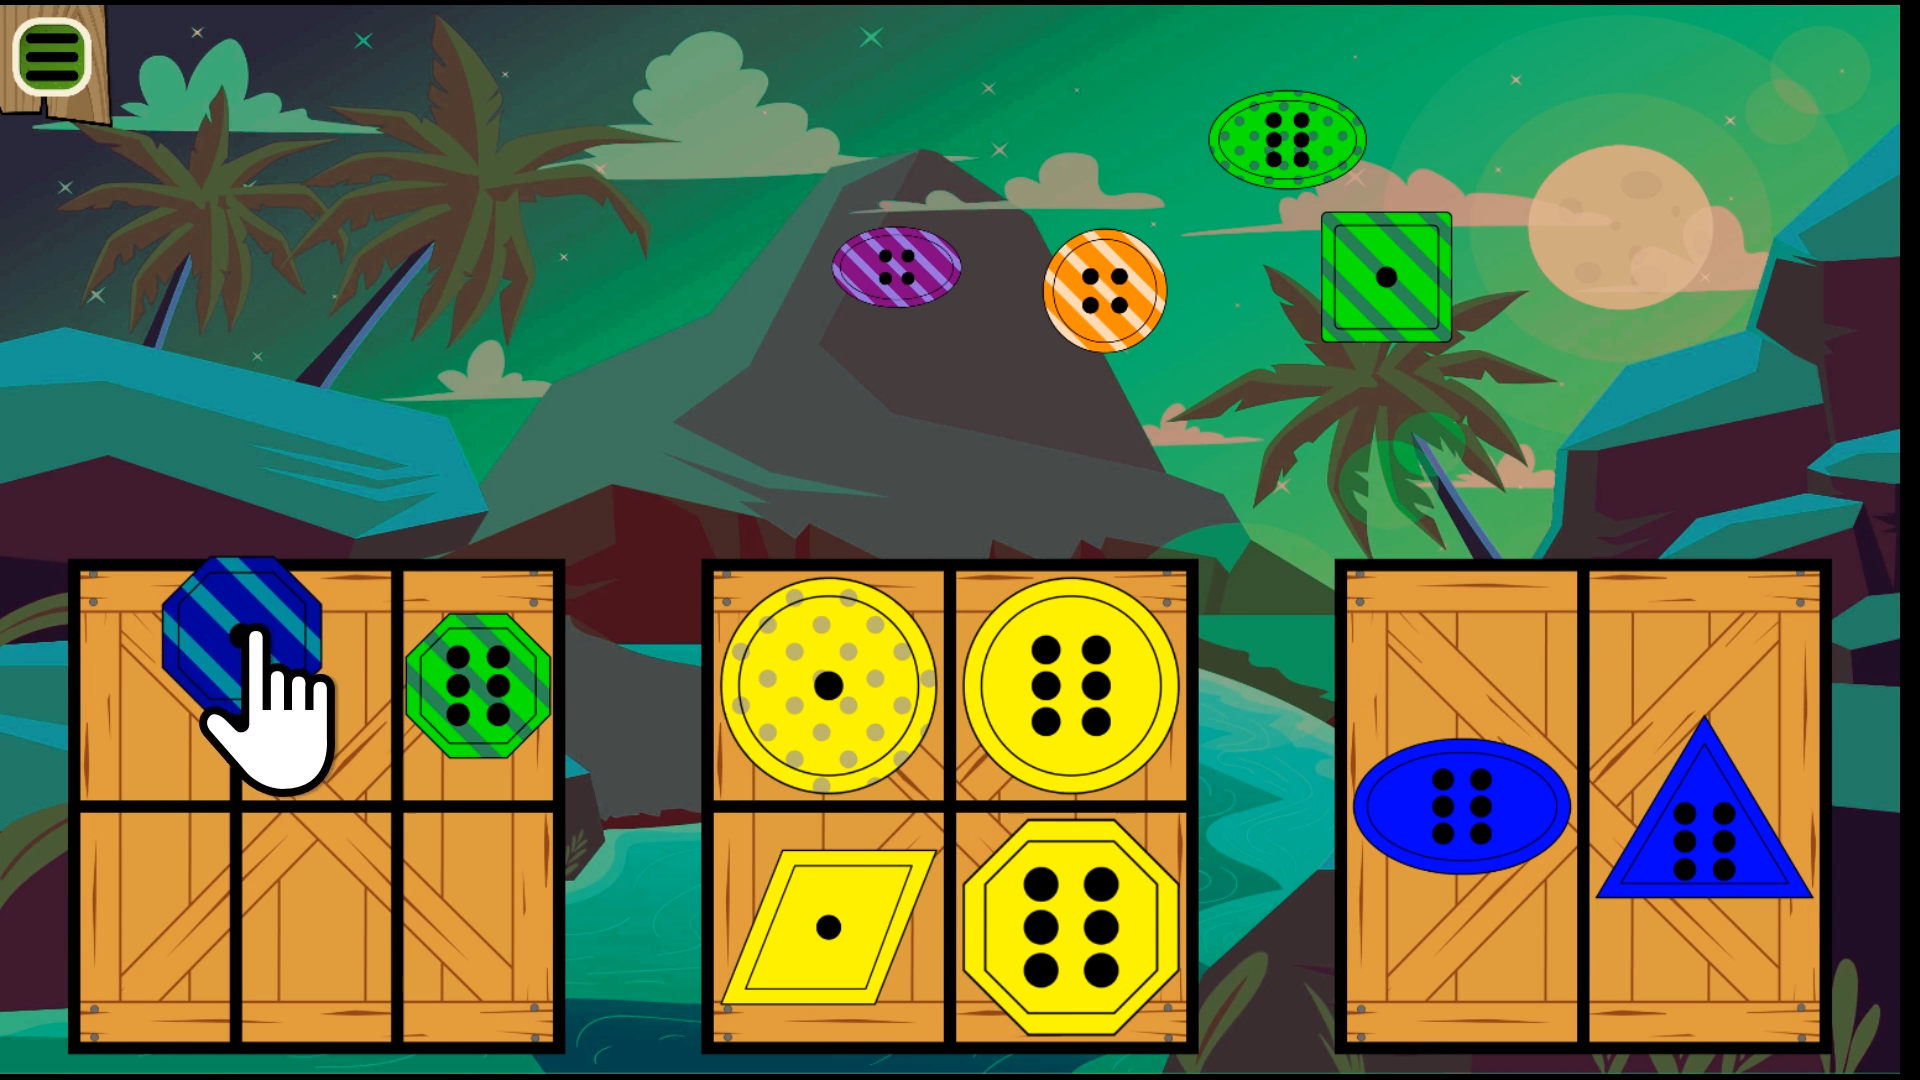
\includegraphics[width=1\textwidth]{figures/restricted1}
    \caption{Restricted Sorting Easy}
    \label{fig:restricted1}
\end{figure}

\begin{figure}[H]
    \centering
    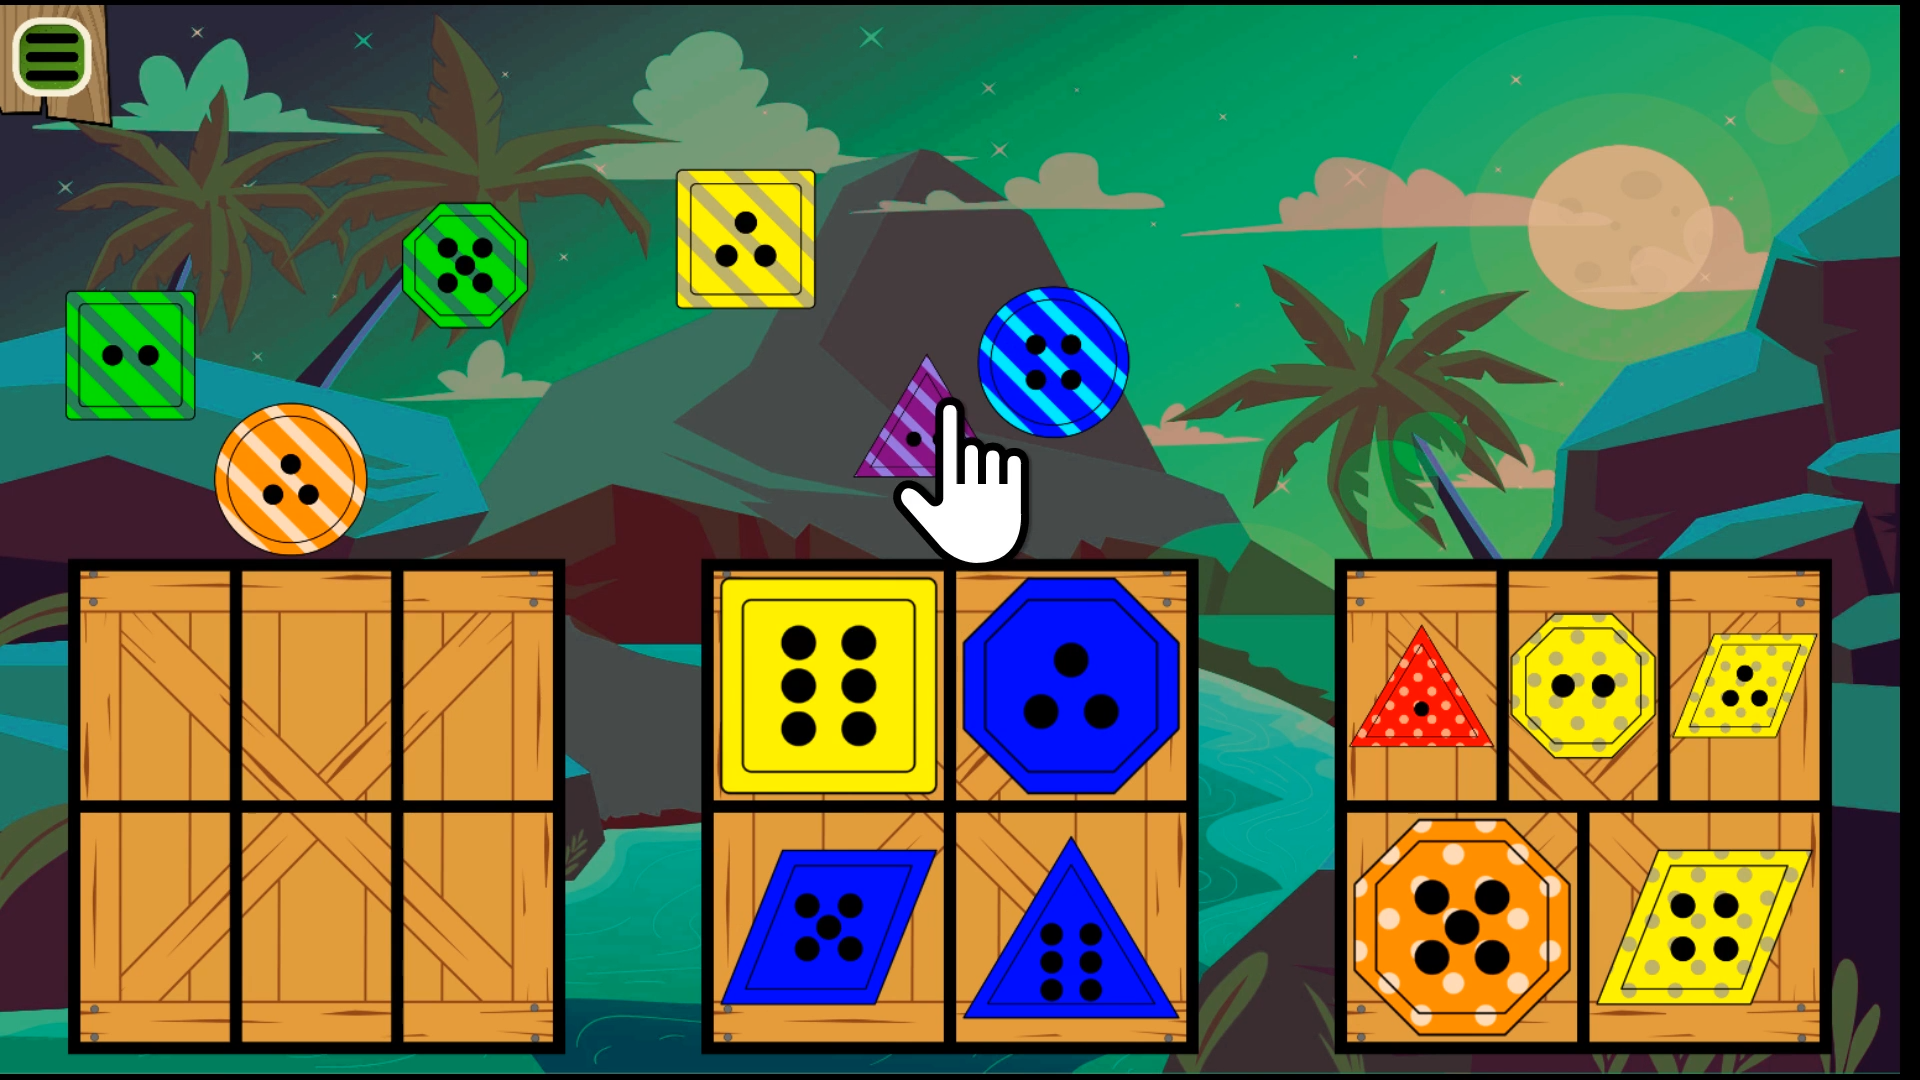
\includegraphics[width=1\textwidth]{figures/restricted2}
    \caption{Restricted Sorting 2 Hard}
    \label{fig:restricted2}
\end{figure}

\begin{figure}[H]
    \centering
    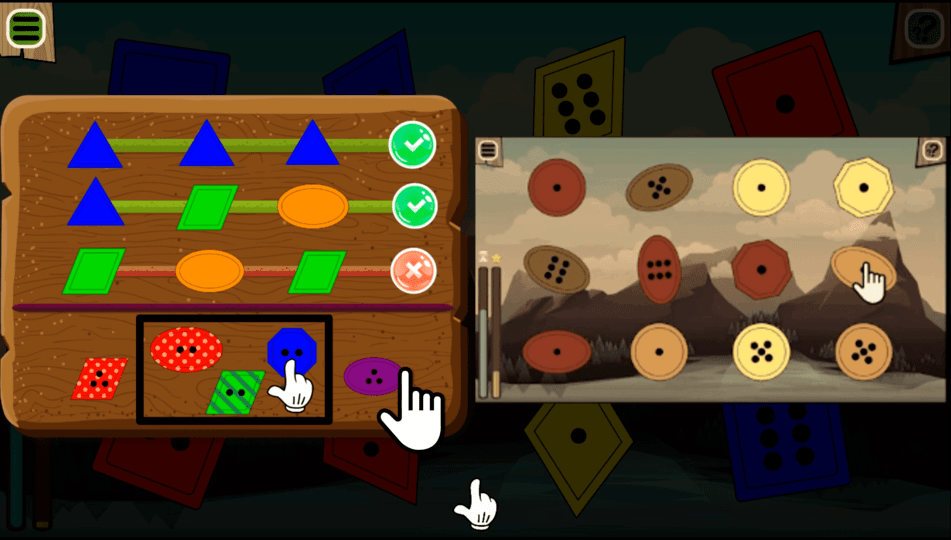
\includegraphics[width=1\textwidth]{figures/introgame}
    \caption{Introduction to Object Pairing Easy}
    \label{fig:introgame}
\end{figure}

\begin{figure}[H]
    \centering
    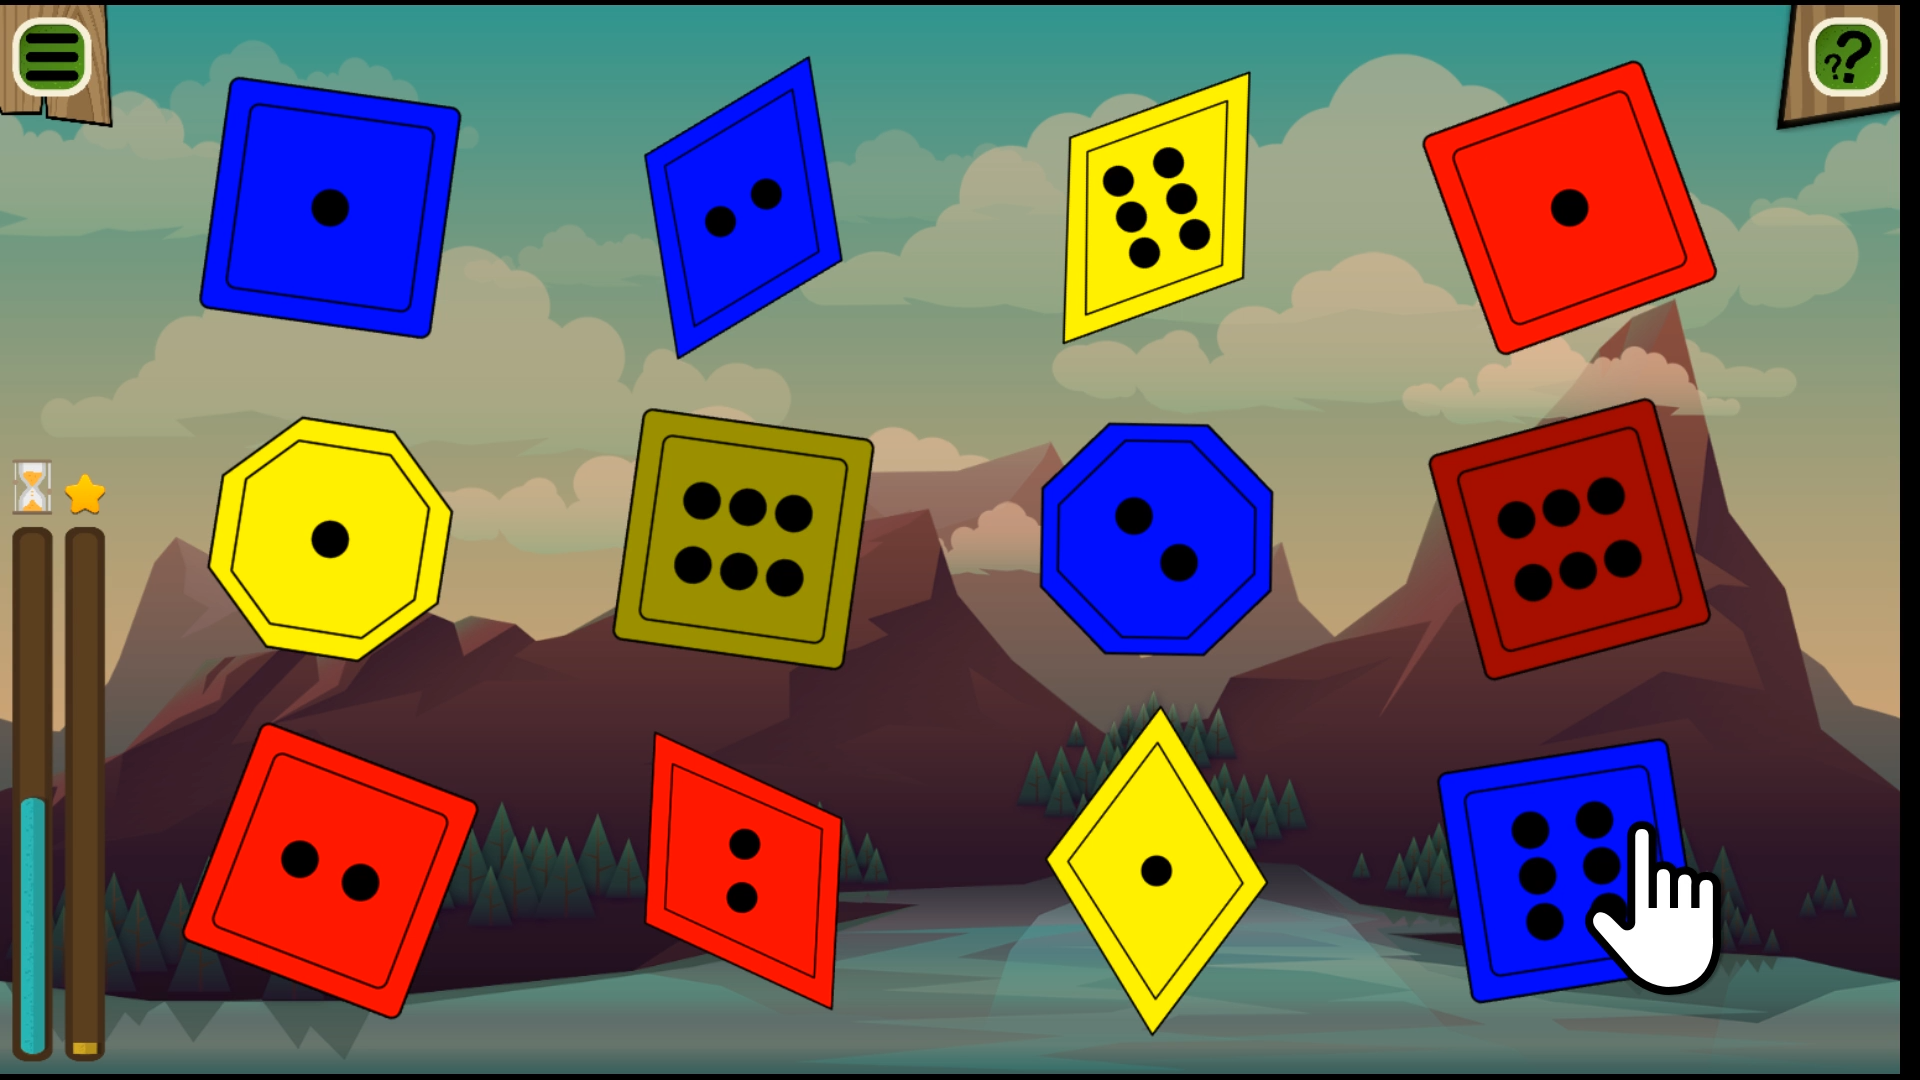
\includegraphics[width=1\textwidth]{figures/gameasy}
    \caption{Object Pairing Easy}
    \label{fig:gameeasy}
\end{figure}

\begin{figure}[H]
    \centering
    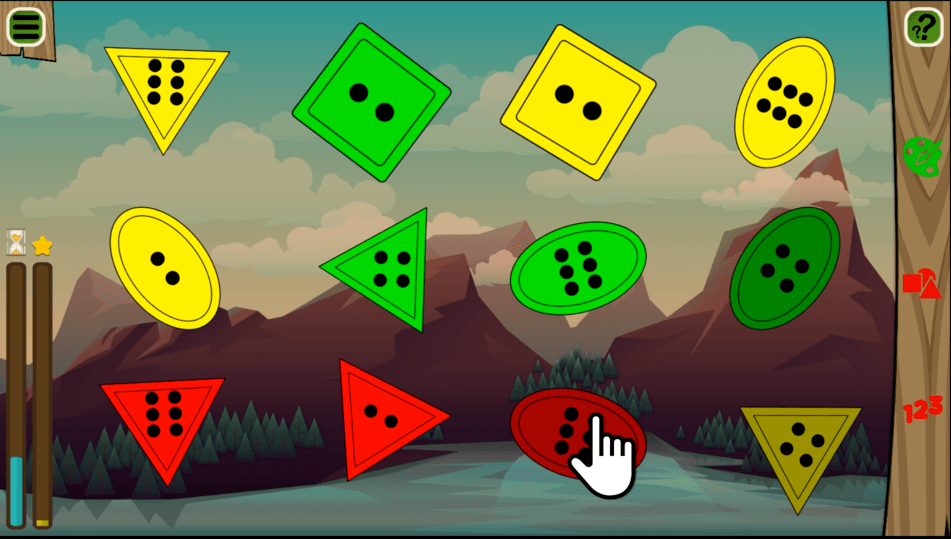
\includegraphics[width=1\textwidth]{figures/gameeasyhelp}
    \caption{Object Pairing Easy Helper Bar}
    \label{fig:gameeasyhelp}
\end{figure}

\begin{figure}[H]
    \centering
    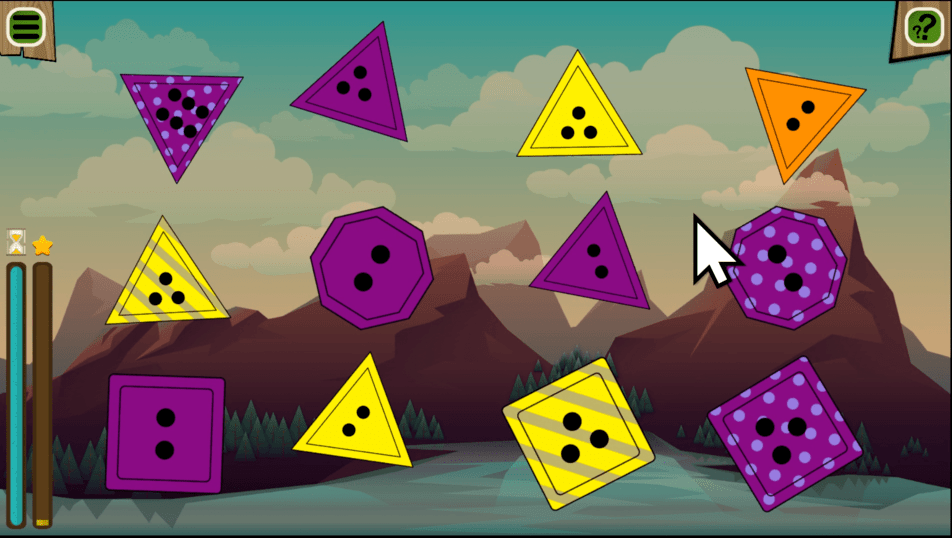
\includegraphics[width=1\textwidth]{figures/gamehard}
    \caption{Object Pairing Hard}
    \label{fig:gamehard}
\end{figure}

\begin{figure}[H]
    \centering
    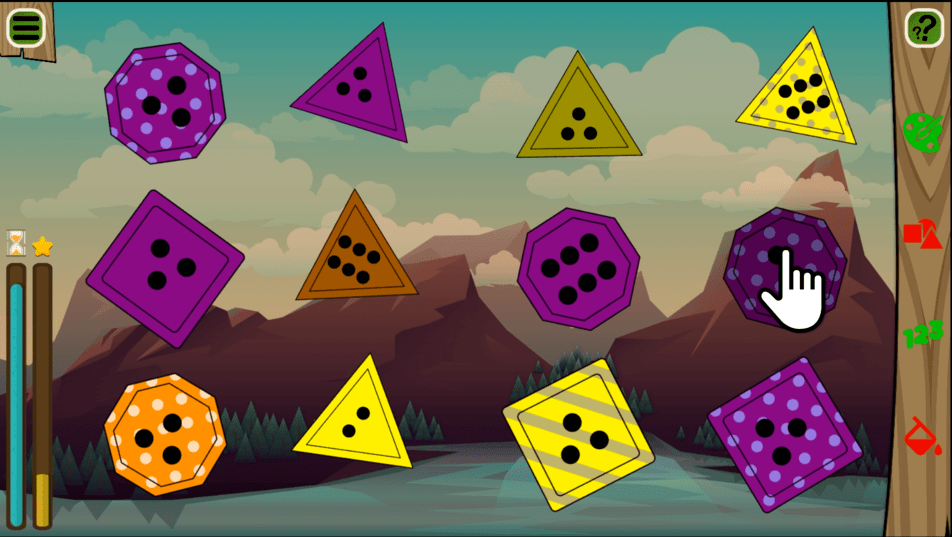
\includegraphics[width=1\textwidth]{figures/gamehardhelp}
    \caption{Object Pairing Hard Helper Bar}
    \label{fig:gamehardhelp}
\end{figure}

\begin{figure}[H]
    \centering
    
\includegraphics[width=1\textwidth]{figures/scorescreen}
    \caption{Score Screen}
    \label{fig:scorescreen}
\end{figure}

% !TEX root = ../thesis.tex

\chapter{Evaluation}
\label{chap:evaluation}
UNDER CONSTRUCTION

In this section the environment the game was tested in will be presented and analysed.
First every game has to be tested on different devices for code errors or functional disbehaviour which was not intended.
Second and third a target and various audience will test the game and significant reaction and behaviour will be stated.

\section{Debugging}
\subsection{Devices}
firefox, chrome, microsoft edge
computer (apple, windows 10), tablet (apple, android), smartphone (apple, android)
\subsection{Differences and obstacles}

\section{Target Audience Test}
5 Test subjects age between 4 and 7 with less to none knowledge of use of electronic devices.
6 Test subjects age between 4 and 7 with strong knowledge of use of electronic devices.

\section{Various Audience Test}
11 Test subjects age between 18 and 40 equally distributed with daily usage of electronics (computer, tablet, smartphone)
13 Test subjects age between 30 and 70 equally distributed with only daily usage of their smartphone

\section{Checklist}
Depending on your budget and available time, you may
have performed simulations or even some experiments. In
either case, it is important to describe the environment
of your experiments or simulations. This includes stating
the parameters and conditions of the environment (sim-
ulated or real), what measurements were taken and how
they were taken.
You need to establish the fact that your simulation or
experiment results are statistically stable, meaning that
they are representative of the space of possible results.
Performing experiments and simulations is a subtle mat-
ter, always putting the validity of your data at risk in
many aspects. Before you perform the simulation or ex-
periment, educate yourself on how to perform simula-
tions, how to interpret the results and how to present
them in graphs and figures.
Each figure (or graph) should be well explained. Dedi-
cate at least one paragraph for each figure. Describe what
the reader sees in each figure and what he should notice.
Moreover, reason on the results - are they the way they
were expected to be? Avoid giving tables of numerical
data as means of presenting your results.
Compare the performance of your solution to the per-
formance of one or two competing solutions. Usually,
when you simulate or experiment on your solution, you
simulate it in contrast to a competing solution. You have
to make sure that the test scenarios are fair and make an
argument about the fairness of your comparison in the
paper.
A special case of experiment is the usability test. Many
times, although the performance of a solution can be im-
pressive, the applicability of it can be minimal. Usability
test is a type of experimentation, which determines the
acceptance of a solution by end-users or its suitability for
certain applications. Usually, papers on software product
solutions contain usability tests.

% !TEX root = ../thesis.tex

\chapter{Conclusion}
\label{chap:conclusion}

The conclusions section, similar to the introduction and
related work sections, serves two purposes. The first is
to elaborate on the impacts of using your approach. The
second is to state limitations or disadvantages of your so-
lution, thus enabling you to provide directions for future
research in the field.



% ---- END MAIN PART ----


\appendix
\clearpage
\renewcommand*{\chapterpagestyle}{myappendixpagestyle}

% !TEX root = ../thesis.tex

% set counter to n-1:
% 2\setcounter{chapter}{0}

\chapter{Gotcha! -- Full Code}\label{ch:gotcha!---full-code}
\section{baseScene.ts}\label{sec:basescene.ts}
\begin{lstlisting}[style=TypeScript, caption={baseScene.ts}]
export class BaseScene extends Phaser.Scene {
    /**
     * Name of the scene
     */
    protected key: string;

    /**
     * Level of the scene
     */
    protected level: number;

    /**
     * Transition graphic
     */
    private transition: Phaser.GameObjects.GameObject[];

    constructor(key: string) {
        super({
            key: key
        });

        this.key = key;
        this.level = 0;
        this.generateNewSeed();
    }

    /**
     * Method for returning the key of this scene
     */
    public getKey(): string {
        return this.key;
    }

    /**
     * Method for returning the key of this scene
     */
    public getLevel(): number {
        return this.level;
    }

    /**
     * Method for generating a new seed so that pseudo randomness is guaranteed
     */
    private generateNewSeed(): void {
        const rndStr: string = Phaser.Math.RND.realInRange(Math.pow(10, 2), Math.pow(10,10)).toString();
        Phaser.Math.RND.sow([rndStr]);
    }

    /**
     * Method for initializing the shape, position and properties of the graphical scene transition
     */
    private transitionInit(): void {
        // Shape of the graphical transition
        const circle: Phaser.GameObjects.Graphics = this.add.graphics();

        // Shape of the screen
        const rectangle: Phaser.GameObjects.Rectangle = this.add.rectangle(0, 0, this.cameras.main.width, this.cameras.main.height, 0x000000);

        // Define circle as the mask
        const mask: Phaser.Display.Masks.GeometryMask = circle.createGeometryMask();

        circle.setPosition(this.cameras.main.width / 2, this.cameras.main.height / 2);
        circle.fillCircle(0, 0, 0.1);
        circle.setDepth(0);

        mask.setInvertAlpha(true);

        rectangle.setDepth(1);
        rectangle.setOrigin(0, 0);
        rectangle.setMask(mask);

        circle.fillCircle(0, 0, 0.1);

        this.transition = [circle, rectangle];
    }

    /**
     * Opening transition. Normally used to visually introduce a new scene
     */
    protected transitionIn(): void {
        // Generating a new seed, so that randomness is guaranteed in every repetition of a scene
        this.generateNewSeed();

        this.transitionInit();

        this.children.bringToTop(this.transition[1]);

        const tween: Phaser.Tweens.Tween = this.add.tween({
            targets: this.transition[0],
            scale: 10 * 0.5 * Math.sqrt(Math.pow(this.cameras.main.width, 2) + Math.pow(this.cameras.main.height, 2)),
            ease: 'linear',
            duration: 700
        });

        tween.on('start', () => this.sound.volume = 0);
        tween.on('complete', () => this.introduction());
        tween.on('update', () => this.sound.volume += 1/tween.duration);
    }

    /**
     * Closing transition. Normally used to visually close or stop a scene.
     * @param scene The scene you want to start next.
     * @param data Additional data you want to give to the next scene.
     */
    protected transitionOut(scene: string, data?: any): void {
        this.children.bringToTop(this.transition[1]);

        const tween: Phaser.Tweens.Tween = this.add.tween({
            targets: this.transition[0],
            scale: 0,
            ease: 'linear',
            duration: 700
        });

        tween.on('complete', () => this.sceneChange(scene, data));
        tween.on('update', () => this.sound.volume -= 1/tween.duration);
    }

    /**
     * Helper method for starting a new scene and stopping the current one
     * as the behaviour of the current scene when starting a new one is
     * not clearly defined in the framework at this point of time.
     * @param scene The scene you want to start next
     * @param data Additional data you want to give to the next scene.
     */
    protected sceneChange(scene: string, data?: any): void {
        this.sound.stopAll();
        this.game.scene.start(scene, data);
        this.game.scene.stop(this.key);
    }

    /**
     * Helper method for playing the introduction and pause the current scene
     */
    protected introduction(): void {
        this.scene.pause();
        this.game.scene.start("IntroScene", {'pausedScene': this.getKey(), 'level': this.getLevel()});
    }

    /**
     * Returns the correct scaling factor for the wanted image size in relation to the real image size.
     * @param wantedImageSize Image size you want to have for a dimension
     * @param realImageSizeWidth The image width you want to scale
     * @param realImageSizeHeight The image height you want to scale
     * @param scaleToHeight Boolean for scaling height or width of image to the wanted size. Default to false.
     */
    protected imageScalingFactor(wantedImageSize: number, realImageSizeWidth: number, realImageSizeHeight: number, scaleToHeight: boolean = false): number {
        let ret: number;
        if (scaleToHeight) {
            ret = Math.max(wantedImageSize / realImageSizeWidth, wantedImageSize / realImageSizeHeight);
        } else {
            ret = Math.min(wantedImageSize / realImageSizeWidth, wantedImageSize / realImageSizeHeight);
        }
        return ret;
    }
}
\end{lstlisting}

\section{preloadAsset.ts}\label{sec:preloadasset.ts}
\begin{lstlisting}[style=TypeScript, caption={preloadAsset.ts}]
import 'phaser';
import {BaseScene} from './baseScene';

export class PreloadAssets extends BaseScene {

    constructor() {
        super('PreloadAssets');
    }

    init(): void {

    }

    preload(): void {
        this.load.setPath('assets/geometrical_objects/');
        this.load.json('objects', 'geometrical_objects.json');

        this.load.setPath('assets/ui/');
        this.load.image('cogwheel', 'cogwheel.png');
        this.load.image('background1', 'background1.png');
    }

    create(): void {
        this.setBackground();
        this.preLoadImages();
        this.preLoadIntroFiles();
        this.preLoadAudio();
        this.initLoadingGraphics();
        this.start();
    }

    /**
     * Method for preloading all asset images
     */
    private preLoadImages(): void {
        // Load category and object images
        const jsonObject: any = this.cache.json.get('objects');

        for (let category of jsonObject['categories']) {
            this.load.setPath('assets/geometrical_objects/categories/');
            this.load.image(category['name'], category['url']);

            this.load.setPath('assets/geometrical_objects/images/');
            for (let property of category['validElements']) {
                for (let url of property['urls']) {
                    this.load.image(url, url);
                }
            }
        }

        for (let image of jsonObject['images']) {
            this.load.image(image['name'], image['name']);
        }

        // Load UI images
        this.load.setPath('assets/ui/');
        //this.load.image('background1', 'background1.png');
        this.load.image('background2', 'background2.png');
        this.load.image('background3', 'background3.png');
        this.load.image('background4', 'background4.png');
        this.load.image('background5', 'background5.png');

        this.load.image('menubackground', 'menu_background.png');

        this.load.spritesheet('fullscreenbuttonblack', 'fullscreen_button_black.png', {frameWidth: 64, frameHeight: 64});
        this.load.image('menubutton', 'menu_button.png');
        this.load.image('help', 'help.png');
        this.load.image('exitbutton', 'exit_button.png');
        this.load.image('replay', 'reload_button.png');
        this.load.image('erase', 'erase_button.png');
        this.load.image('return', 'return_button.png');

        this.load.image('star_0', 'star_0.png');
        this.load.image('star_1', 'star_1.png');
        this.load.image('star_2', 'star_2.png');
        this.load.image('star_3', 'star_3.png');

        this.load.image('timefluid', 'timefluid.png');
        this.load.image('gamefluid', 'gamefluid.png');
        this.load.image('progressstar', 'star.png');
        this.load.image('progressbar', 'progressbar.png');
        this.load.image('progressbarGreen', 'progressbar_green.png');
        this.load.image('progressbarRed', 'progressbar_red.png');
        this.load.image('plus', 'plus.png');
        this.load.image('minus', 'minus.png');


        this.load.image('hourglass', 'hourglass.png');
        this.load.image('finger', 'finger.png');


        this.load.image('crate', 'crate_topview.png');
        this.load.image('wooden_crate', 'wooden_crate.png');

        this.load.image('title', 'title.png');

        this.load.image('catButton', 'cat_button.png');
        this.load.image('levelButton11', 'level11_button.png');
        this.load.image('levelButton12', 'level12_button.png');
        this.load.image('levelButton13', 'level13_button.png');
        this.load.image('levelButton14', 'level14_button.png');
        this.load.image('levelButton21', 'level21_button.png');
        this.load.image('levelButton22', 'level22_button.png');
        this.load.image('levelButton23', 'level23_button.png');
        this.load.image('levelButton24', 'level24_button.png');
        this.load.image('levelButton31', 'level31_button.png');
        this.load.image('levelButton32', 'level32_button.png');
        this.load.image('levelButton33', 'level33_button.png');
        this.load.image('levelButton34', 'level34_button.png');
    }

    /**
     * Method for preloading all introduction files
     */
    private preLoadIntroFiles(): void {
        this.load.setPath('assets/introduction/');
        this.load.image('intro_set', 'intro_set.png');
        this.load.spritesheet('intro_sorting', 'intro_sorting.png', {frameWidth: 336, frameHeight: 189, endFrame: 150});
        this.load.spritesheet('intro_falling', 'intro_falling.png', {frameWidth: 336, frameHeight: 189, endFrame: 68});
        this.load.spritesheet('intro_restricted', 'intro_restricted.png', {frameWidth: 336, frameHeight: 189, endFrame: 201});
        this.load.spritesheet('intro_set_easy', 'intro_set_easy.png', {frameWidth: 336, frameHeight: 189, endFrame: 225});
        this.load.spritesheet('intro_set_hard', 'intro_set_hard.png', {frameWidth: 336, frameHeight: 189, endFrame: 68});
    }

    /**
     * Method for preloading all audio files
     */
    private preLoadAudio(): void {
        this.load.setPath('assets/ui_audio/');
        this.load.audio('back', 'back.mp3');
        this.load.audio('battle', 'battle.mp3');
        this.load.audio('exploration', 'exploration.mp3');
        this.load.audio('fun', 'fun.mp3');
        this.load.audio('loading', 'loading.mp3');
        this.load.audio('lose', 'lose.mp3');
        this.load.audio('pause', 'pause.mp3');
        this.load.audio('select', 'select.mp3');
        this.load.audio('space', 'space.mp3');
        this.load.audio('sparkle', 'sparkle.mp3');
        this.load.audio('welcome', 'welcome.mp3');
        this.load.audio('win', 'win.mp3');
    }

    /**
     * Method for initializing the loading graphics/animation
     */
    private initLoadingGraphics(): void {
        // Loading graphics
        const cogwheel: Phaser.GameObjects.Sprite = this.add.sprite(1/2*this.cameras.main.width, 1/3*this.cameras.main.height, 'cogwheel');
        cogwheel.setOrigin(0.5, 0.5);
        const scale: number = this.imageScalingFactor(1/3*Math.min(this.cameras.main.height, this.cameras.main.width), cogwheel.width, cogwheel.height);
        cogwheel.setScale(scale);

        const cogTween: Phaser.Tweens.Tween = this.tweens.add({
            targets: cogwheel,
            angle: 360,
            ease: 'Linear',
            repeat: -1,
            duration: 5000
        });

        // Progress bar
        const progress = this.add.graphics();

        this.load.on('progress', function (value) {
            progress.clear();
            progress.fillStyle(0xffffff, 1);
            progress.fillRect(20, 4/5*this.cameras.main.height, (this.cameras.main.width - 40) * value, 1/10*this.cameras.main.height);
        }, this);
    }

    /**
     * Method for initializing the loading and action on completion
     */
    private start(): void {
        this.load.on('complete', function(){
            this.sceneChange('DropDownMenu');
        }, this);

        this.load.start();
    }

    /**
     * Method for initializing the background
     */
    private setBackground(): void {
        let background = this.add.sprite(0, 0, 'background1');
        background.setOrigin(0, 0);
        background.setDisplaySize(this.cameras.main.width, this.cameras.main.height);
        background.setAlpha(0.3);
    }
}
\end{lstlisting}

\section{dropDownMenu.ts}\label{sec:dropdownmenu.ts}
\begin{lstlisting}[style=TypeScript, caption={dropDownMenu.ts}]
import 'phaser';
import {BaseScene} from './baseScene';

export class DropDownMenu extends BaseScene {

    /**
     * Name of the paused scene
     */
    private key_paused_scene: string;

    /**
     * Lock for not messing up animations by clicking repeatedly without waiting for the animation to finish
     */
    private lock: boolean;

    /**
     * State of the drop down menu
     */
    private menuDown: boolean;

    /**
     * Size of the menu buttons
     */
    private buttonSize: number;

    /**
     * Menu button
     */
    private menuButton: Phaser.GameObjects.Sprite;

    /**
     * Exit button
     */
    private exitButton: Phaser.GameObjects.Sprite;

    /**
     * Fullscreen switch
     */
    private fullscreenButton: Phaser.GameObjects.Sprite;

    /**
     * Menu background
     */
    private menuBackground: Phaser.GameObjects.Sprite;

    /**
     * Pause background
     */
    private pauseBackground: Phaser.GameObjects.Container;

    constructor() {
        super('DropDownMenu');
    }

    init(): void {
        // Initialize fields
        this.pauseBackground = this.add.container(0, 0);
        this.key_paused_scene = null;
        this.lock = false;
        this.menuDown = false;
        this.buttonSize = 64;
    }

    preload(): void {

    }

    create(): void {
        this.setPixelScreen();
        this.setMenu();
        this.initInput();
    }

    update(time: number, delta: number): void {

    }

    /**
     * Method for initializing the menu buttons, background and action
     */
    private setMenu(): void {
        let scale: number;

        // Menubackground
        this.menuBackground = this.add.sprite(10 + 64 + 25, 100, 'menubackground');
        this.menuBackground.setOrigin(1, 1);
        this.menuBackground.setDisplaySize(200, 80 * 5);
        this.menuBackground.setTint(0xeeeeee);

        // ExitButton
        this.exitButton = this.add.sprite(-64, 10 + 32 + 2 * (10 + 64), 'exitbutton');
        this.exitButton.setOrigin(0.5, 0.5);
        this.exitButton.setName("exitButton");
        this.exitButton.setData('clicked', false);

        scale = this.imageScalingFactor(this.buttonSize, this.exitButton.width, this.exitButton.height);
        this.exitButton.setScale(scale);

        this.exitButton.setInteractive({cursor: 'pointer'});

        // Fullscreen Button
        this.fullscreenButton = this.add.sprite(-64, 10 + 32 + (10 + 64), 'fullscreenbuttonblack', 0);
        this.fullscreenButton.setOrigin(0.5, 0.5);

        scale = this.imageScalingFactor(this.buttonSize, this.fullscreenButton.width, this.fullscreenButton.height);
        this.fullscreenButton.setScale(scale);

        this.fullscreenButton.setName("fullscreenButton");
        this.fullscreenButton.setData('clicked', false);

        this.fullscreenButton.setInteractive({cursor: 'pointer'});

        // Enable key F for enabling/disabling fullscreen
        const FKey: Phaser.Input.Keyboard.Key = this.input.keyboard.addKey('F');
        FKey.on('down', function () {
            this.scale.toggleFullscreen();
            if (this.scale.isFullscreen) {
                this.fullscreenButton.setFrame(0);
            } else {
                this.fullscreenButton.setFrame(1);
            }

        }, this);

        // MenuButton
        this.menuButton = this.add.sprite(32 + 10, 10 + 32, 'menubutton');
        this.menuButton.setOrigin(0.5, 0.5);

        scale = this.imageScalingFactor(this.buttonSize, this.menuButton.width, this.menuButton.height);
        this.menuButton.setScale(scale);

        this.menuButton.setName("menuButton");
        this.menuButton.setData('clicked', false);

        this.menuButton.setInteractive({cursor: 'pointer'});

        // StartGame
        this.game.scene.start('WelcomeScene');
    }

    /**
     * Method for initializing all input
     */
    private initInput(): void {
        this.input.on('pointerdown', function (pointer, currentlyOver) {
            const gameObject: any = currentlyOver[0];
            if (gameObject instanceof Phaser.GameObjects.Sprite) {
                gameObject.setData('clicked', true);
            }
        }, this);

        this.input.on('pointerup', function (pointer, currentlyOver) {
            const gameObject: any = currentlyOver[0];
            if (gameObject instanceof Phaser.GameObjects.Sprite && gameObject.getData('clicked')) {
                this.buttonFunction(gameObject);
            }

            this.menuButton.setData("clicked", false);
            this.exitButton.setData("clicked", false);
            this.fullscreenButton.setData("clicked", false);

        }, this);
    }

    /**
     * Method for assigning each button an event function
     * @param gameObject GameObject on which you want the function on
     */
    private buttonFunction(gameObject: Phaser.GameObjects.Sprite): void {
        switch (gameObject.name) {
            case 'menuButton': {
                if (!this.lock) {
                    // Acquire lock
                    this.lock = true;
                    this.menuAction();
                }
                break;
            }

            case 'fullscreenButton': {
                this.scale.toggleFullscreen();

                if (this.scale.isFullscreen) {
                    gameObject.setFrame(0);
                } else {
                    gameObject.setFrame(1);
                }
                break;
            }

            case 'exitButton': {
                this.menuAction();

                this.game.scene.getScenes(false).forEach(function (scene) {
                    // @ts-ignore
                    const sceneKey: string = scene.key;
                    if (!(sceneKey === this.getKey()) && (this.game.scene.isActive(sceneKey) || this.game.scene.isPaused(sceneKey))) {
                        scene.sound.stopAll();
                        this.game.scene.stop(sceneKey);
                    }
                }, this);

                if (this.key_paused_scene === 'LevelMenuScene' || this.key_paused_scene === 'WelcomeScene') {
                    this.game.scene.start('WelcomeScene');
                } else {
                    this.game.scene.start('LevelMenuScene');
                }
                break;
            }

            default: {
                break;
            }
        }
    }

    /**
     * Method which defines the graphical behaviour of the drop down menu
     */
    private menuAction(): void {

        if (this.menuDown) {
            // Animation
            const menuButtonTween: Phaser.Tweens.Tween = this.tweens.add({
                targets: this.menuButton,
                angle: 0,
                ease: 'Cubic',
                duration: 700,
                onComplete: () => this.lock = false
            });

            const menuBackgroundTween: Phaser.Tweens.Tween = this.tweens.add({
                targets: this.menuBackground,
                y: 100,
                ease: 'Cubic',
                duration: 500,
                delay: 200
            });

            const fullscreenButtonTween: Phaser.Tweens.Tween = this.tweens.add({
                targets: this.fullscreenButton,
                x: -64,
                ease: 'Cubic',
                duration: 500,
                delay: 100
            });

            const exitButtonTween: Phaser.Tweens.Tween = this.tweens.add({
                targets: this.exitButton,
                x: -64,
                ease: 'Cubic',
                duration: 500
            });

            const pixelScreenTween: Phaser.Tweens.Tween = this.tweens.add({
                targets: this.pauseBackground.getAll(),
                alpha: 0,
                ease: 'linear',
                duration: 700,
                delay: 0,
                onComplete: () => this.pauseBackground.setVisible(false)
            });

            this.menuDown = false;

            // Resume current scene
            this.game.scene.resume(this.key_paused_scene);

        } else {
            // Pause current scene
            this.sound.add('pause').play();

            // @ts-ignore
            const key_paused_scene: string = this.game.scene.getScenes(true)[0].key;
            this.game.scene.pause(key_paused_scene);
            this.key_paused_scene = key_paused_scene;

            // Animation
            const menuButtonTween: Phaser.Tweens.Tween = this.tweens.add({
                targets: this.menuButton,
                angle: -90,
                ease: 'Cubic',
                duration: 700,
                onComplete: () => this.lock = false,
            });

            const menuBackgroundTween: Phaser.Tweens.Tween = this.tweens.add({
                targets: this.menuBackground,
                y: 3 * (64 + 10) + 30,
                ease: 'Cubic',
                duration: 600
            });

            const fullscreenButtonTween: Phaser.Tweens.Tween = this.tweens.add({
                targets: this.fullscreenButton,
                x: 10 + 32,
                ease: 'Cubic',
                duration: 500,
                delay: 100,
            });

            const exitButtonTween: Phaser.Tweens.Tween = this.tweens.add({
                targets: this.exitButton,
                x: 10 + 32,
                ease: 'Cubic',
                duration: 500,
                delay: 200
            });

            this.pauseBackground.setVisible(true);

            const pixelScreenTween: Phaser.Tweens.Tween = this.tweens.add({
                targets: this.pauseBackground.getAll(),
                alpha: 0.9,
                ease: 'linear',
                duration: 700,
                delay: 0
            });

            this.menuDown = true;
        }
    }

    /**
     * Method for setting the pixeled overlay and the hourglass
     */
    private setPixelScreen(): void {
        const pixelScreen: Phaser.GameObjects.Grid = this.add.grid(0, 0, this.cameras.main.width, this.cameras.main.height, this.cameras.main.width / 100, this.cameras.main.width / 100);
        pixelScreen.setOrigin(0, 0);
        pixelScreen.setFillStyle(0x777777);
        pixelScreen.setAltFillStyle(0x555555);
        pixelScreen.setOutlineStyle(0x555555);
        pixelScreen.setAlpha(0);
        this.pauseBackground.add(pixelScreen);

        const hourglass: Phaser.GameObjects.Sprite = this.add.sprite(this.cameras.main.width / 2, this.cameras.main.height / 2, 'hourglass');
        hourglass.setOrigin(0.5, 0.5);

        const clockScale: number = this.imageScalingFactor(3 / 5 * this.cameras.main.height, hourglass.width, hourglass.height);
        hourglass.setScale(clockScale);
        hourglass.setAlpha(0);

        this.pauseBackground.add(hourglass);

        this.pauseBackground.setVisible(false);
        this.children.sendToBack(this.pauseBackground);
    }
}
\end{lstlisting}

\section{introScene.ts}\label{sec:introscene.ts}
\begin{lstlisting}[style=TypeScript, caption={introScene.ts}]
import 'phaser';
import {BaseScene} from './baseScene';
import AnimationManager = Phaser.Animations.AnimationManager;

export class IntroScene extends BaseScene {

    /**
     * Name of the paused scene the intro is currently playing for
     */
    private pausedScene: string;

    /**
     * Boolean, indicating if the paused scene should be resumed
     */
    private resume: boolean;

    constructor() {
        super('IntroScene');
    }

    init(data): void {
        this.pausedScene = data.pausedScene;
        this.level = data.level;
        this.resume = false;
    }

    preload(): void {

    }

    create(): void {
        // Bring MenuUI to the front and initialize transition
        this.game.scene.sendToBack(this.getKey());
        this.game.scene.moveUp(this.getKey());

        if (this.getIntroData() == null) {
            this.scene.resume(this.pausedScene);
            this.scene.stop(this.getKey());
        } else {
            this.initIntro();
        }

    }

    /**
     * Method for initializing the introduction objects and animation
     */
    private initIntro(): void {
        const background: Phaser.GameObjects.Rectangle = this.setBackground();
        const intro: Phaser.GameObjects.Sprite = this.setIntro();

        const finger: Phaser.GameObjects.Sprite = this.add.sprite(this.cameras.main.width/2, this.cameras.main.height-10, 'finger');
        const scale: number = this.imageScalingFactor(this.cameras.main.height/10, finger.width, finger.height);
        finger.setScale(scale);
        finger.setOrigin(0.5, 1);

        if (this.pausedScene === "GameScene"){
            intro.setX(3/4*this.cameras.main.width);
            const intro1scale: number = this.imageScalingFactor(this.cameras.main.width/2, intro.width, intro.height);
            intro.setScale(intro1scale);

            const intro2: Phaser.GameObjects.Sprite = this.add.sprite(1/4*this.cameras.main.width, 0, 'intro_set');
            intro2.setOrigin(0.5, 0.5);
            const intro2scale: number = this.imageScalingFactor(this.cameras.main.width/2, intro2.width, intro2.height);
            intro2.setScale(intro2scale);

            this.setAnimation(intro, background, finger, intro2);
        } else {
            this.setAnimation(intro, background, finger);
        }
    }

    /**
     * Method for the input setup
     * @param intro Introduction image
     * @param background Background image
     * @param finger Finger image
     * @param intro2 Introduction 2 image
     */
    private initInput(intro: Phaser.GameObjects.Sprite, background: Phaser.GameObjects.Rectangle, finger: Phaser.GameObjects.Sprite, intro2?: Phaser.GameObjects.Sprite): void {
        this.input.on('pointerdown', function () {
            this.input.on('pointerup', function () {
                this.resume = true;
                const introTweenOut: Phaser.Tweens.Tween = this.tweens.add({
                    targets: intro,
                    y: -300,
                    ease: 'linear',
                    duration: 200,
                    onComplete: function () {
                        this.scene.resume(this.pausedScene);
                        this.scene.stop(this.getKey());
                    }.bind(this)
                });

                if (this.pausedScene === "GameScene") {
                    const intro2TweenIn: Phaser.Tweens.Tween = this.tweens.add({
                        targets: intro2,
                        y: -300,
                        ease: 'linear',
                        duration: 200
                    });
                }

                const backgroundTweenOut: Phaser.Tweens.Tween = this.tweens.add({
                    targets: background,
                    alpha: 0.01,
                    ease: 'linear',
                    duration: 200
                });

                const fingerTweenOut: Phaser.Tweens.Tween = this.tweens.add({
                    targets: finger,
                    alpha: 0.01,
                    ease: 'linear',
                    duration: 200
                });

            }, this);
        }, this);
    }

    /**
     * Method for generating the background object
     */
    private setBackground(): Phaser.GameObjects.Rectangle {
        const background: Phaser.GameObjects.Rectangle = this.add.rectangle(0, 0, this.cameras.main.width, this.cameras.main.height);
        background.setOrigin(0, 0);
        background.setFillStyle(0x000000);
        background.setAlpha(0.01);

        return background;
    }

    /**
     * Method for generating the introduction object
     */
    private setIntro(): Phaser.GameObjects.Sprite {
        const data: [string, Phaser.Types.Animations.GenerateFrameNumbers] = this.getIntroData();

        const introConfig = {
            key: 'animateGif',
            frames: this.anims.generateFrameNumbers(data[0], data[1]),
            frameRate: 20,
            repeat: -1
        };

        if(this.anims.exists(introConfig.key)) {
            this.anims.remove(introConfig.key)
        }

        this.anims.create(introConfig);

        const intro: Phaser.GameObjects.Sprite = this.add.sprite(this.cameras.main.width / 2, this.cameras.main.height / 2, data[0]);
        intro.setOrigin(0.5, 0.5);

        const scale: number = this.imageScalingFactor(this.cameras.main.width * 4 / 5, intro.width, intro.height);
        intro.setScale(scale);

        intro.setY(0);

        return intro;
    }

    /**
     * Method for the animation setup
     * @param intro The introduction gif/spritesheet
     * @param background The background
     * @param finger Finger image
     * @param intro2 The 2nd introduction gif/spritesheet
     */
    private setAnimation(intro: Phaser.GameObjects.Sprite, background: Phaser.GameObjects.Rectangle, finger: Phaser.GameObjects.Sprite, intro2?: Phaser.GameObjects.Sprite) {
        const introTweenIn: Phaser.Tweens.Tween = this.tweens.add({
            targets: intro,
            y: this.cameras.main.height / 2,
            ease: 'linear',
            duration: 500,
            onComplete: function(){
                if (this.pausedScene === "GameScene") {
                    this.initInput(intro, background, finger, intro2)
                } else {
                    this.initInput(intro, background, finger)
                }
            }.bind(this)
        });

        if (this.pausedScene === "GameScene") {
            const intro2TweenIn: Phaser.Tweens.Tween = this.tweens.add({
                targets: intro2,
                y: this.cameras.main.height / 2,
                ease: 'linear',
                duration: 500
            });
        }

        const backgroundTweenIn: Phaser.Tweens.Tween = this.tweens.add({
            targets: background,
            alpha: 0.8,
            ease: 'linear',
            duration: 500
        });

        const fingerTween: Phaser.Tweens.Tween = this.tweens.add({
            targets: finger,
            alpha: 0.1,
            ease: 'Linear',
            repeat: 1000,
            yoyo: true,
            duration: 1000
        });

        intro.play('animateGif');
    }

    /**
     * Method for retrieving the correct introduction for the current scene
     */
    private getIntroData(): [string, Phaser.Types.Animations.GenerateFrameNumbers] {
        let ret: [string, Phaser.Types.Animations.GenerateFrameNumbers];

        switch (this.pausedScene + String(this.getLevel())) {
            case 'PropertySortingScene1': {
                ret = ['intro_sorting', {start: 0, end: 150, first: 150}];
                break;
            }

            case 'PropertySortingScene2': {
                ret = ['intro_sorting', {start: 0, end: 150, first: 150}];
                break;
            }

            case 'PropertySortingScene3': {
                ret = ['intro_sorting', {start: 0, end: 150, first: 150}];
                break;
            }

            case 'PropertySortingScene4': {
                ret = ['intro_sorting', {start: 0, end: 150, first: 150}];
                break;
            }

            case 'PropertySortingScene5': {
                ret = ['intro_falling', {start: 0, end: 68, first: 68}];
                break;
            }

            case 'PropertySortingScene6': {
                ret = ['intro_falling', {start: 0, end: 68, first: 68}];
                break;
            }

            case 'PropertySortingScene7': {
                ret = ['intro_falling', {start: 0, end: 68, first: 68}];
                break;
            }

            case 'PropertySortingScene8': {
                ret = ['intro_falling', {start: 0, end: 68, first: 68}];
                break;
            }

            case 'RestrictedSortingScene1': {
                ret = ['intro_restricted', {start: 0, end: 201, first: 201}];
                break;
            }

            case 'RestrictedSortingScene2': {
                ret = ['intro_restricted', {start: 0, end: 201, first: 201}];
                break;
            }

            case 'GameScene1': {
                ret = ['intro_set_easy', {start: 0, end: 225, first: 225}];
                break;
            }

            case 'GameScene2': {
                ret = ['intro_set_hard', {start: 0, end: 68, first: 68}];
                break;
            }

            default: {
                ret = null;
                break;
            }
        }
        return ret;
    }
}
\end{lstlisting}

\section{welcomeScene.ts}\label{sec:welcomescene.ts}
\begin{lstlisting}[style=TypeScript, caption={}]
import 'phaser';
import {BaseScene} from './baseScene';

export class WelcomeScene extends BaseScene {

    constructor() {
        super('WelcomeScene');
    }

    init(): void {

    }

    preload(): void {

    }

    create(): void {
        // Bring MenuUI to the front and initialize transition
        this.game.scene.sendToBack(this.getKey());
        this.transitionIn();

        this.setBackground();
        this.setTitle();
        this.initInput();
        this.initAudio();
    }

    /**
     * Method for initializing the background
     */
    private setBackground(): void {
        let background = this.add.sprite(0, 0, 'background1');
        background.setOrigin(0, 0);
        background.setDisplaySize(this.cameras.main.width, this.cameras.main.height);
        background.setInteractive({ cursor: 'pointer' });
    }

    /**
     * Method for initializing title and animation
     */
    private setTitle(): void {
        // Add title
        const title: Phaser.GameObjects.Sprite = this.add.sprite(this.cameras.main.width / 2, this.cameras.main.height / 2, 'title');
        const titleScale: number = this.imageScalingFactor(4/6*this.cameras.main.width, title.width, title.height);
        title.setOrigin(0.5, 0.5);
        title.setScale(titleScale);
        title.setInteractive({ cursor: 'pointer' });

        const titleTween: Phaser.Tweens.Tween = this.tweens.add({
            targets: title,
            alpha: 0.7,
            ease: 'Linear',
            repeat: 1000,
            yoyo: true,
            duration: 1000
        });

        // Add finger
        const finger: Phaser.GameObjects.Sprite = this.add.sprite(this.cameras.main.width / 2, 3/4*this.cameras.main.height, 'finger');
        const fingerScale: number = this.imageScalingFactor(1/6*this.cameras.main.height, finger.width, finger.height, true);
        finger.setOrigin(0.5, 0.5);
        finger.setScale(fingerScale);
        finger.setInteractive({ cursor: 'pointer' });

        const fingerTween: Phaser.Tweens.Tween = this.tweens.add({
            targets: finger,
            alpha: 0.1,
            ease: 'Linear',
            repeat: 1000,
            yoyo: true,
            duration: 1000
        });
    }

    /**
     * Method for initializing event actions
     */
    private initInput(): void {
        this.input.on('pointerdown', function(){
            this.input.on('pointerup', () => this.transitionOut('LevelMenuScene'));
        }, this);
    }

    /**
     * Method for initializing sound effects
     */
    private initAudio(): void {
        this.sound.add('welcome').play('', {loop: true});
    }
}
\end{lstlisting}

\section{levelMenuScene.ts}\label{sec:levelmenuscene.ts}
\begin{lstlisting}[style=TypeScript, caption={levelMenuScene.ts}]
import 'phaser';
import {BaseScene} from './baseScene';

export class LevelMenuScene extends BaseScene {
    /**
     * Group with all level buttons
     */
    private levelButtons: Phaser.GameObjects.Group;

    /**
     * Global size of all buttons
     */
    private buttonSize: number;

    constructor() {
        super('LevelMenuScene');
    }

    init(): void {
        // Initialize fields
        this.levelButtons = this.add.group();

        // Define button size dependant on the screen dimensions and the number of buttons
        this.buttonSize = Math.min(this.cameras.main.width / (4 + 2), this.cameras.main.height / (3 + 2));
    }

    preload(): void {

    }

    create(): void {
        // Bring MenuUI to the front and initialize transition
        this.game.scene.sendToBack(this.getKey());
        this.transitionIn();

        this.setBackground();
        this.setTitle();
        this.setVisualLink();
        this.setLevelButtons();
        this.setStars();
        this.initInput();
        this.initAudio();
    }

    update(time: number): void {

    }

    /**
     * Method for initializing background graphics
     */
    private setBackground(): void {
        const background: Phaser.GameObjects.Sprite = this.add.sprite(0, 0, 'background1');
        background.setOrigin(0, 0);
        background.setDisplaySize(this.cameras.main.width, this.cameras.main.height);
    }

    /**
     * Method for initializing the level buttons and their onclick action
     */
    private setLevelButtons(): void {
        const catButton: Phaser.GameObjects.Sprite = this.add.sprite(20, this.cameras.main.height - 20, 'catButton');
        const eraseButton: Phaser.GameObjects.Sprite = this.add.sprite(this.cameras.main.width - 20, this.cameras.main.height - 20, 'erase');
        const levelButton11: Phaser.GameObjects.Sprite = this.add.sprite(1 / 5 * this.cameras.main.width, 1 / 4 * this.cameras.main.height, 'levelButton11');
        const levelButton12: Phaser.GameObjects.Sprite = this.add.sprite(2 / 5 * this.cameras.main.width, 1 / 4 * this.cameras.main.height, 'levelButton12');
        const levelButton13: Phaser.GameObjects.Sprite = this.add.sprite(3 / 5 * this.cameras.main.width, 1 / 4 * this.cameras.main.height, 'levelButton13');
        const levelButton14: Phaser.GameObjects.Sprite = this.add.sprite(4 / 5 * this.cameras.main.width, 1 / 4 * this.cameras.main.height, 'levelButton14');
        const levelButton21: Phaser.GameObjects.Sprite = this.add.sprite(4 / 5 * this.cameras.main.width, 2 / 4 * this.cameras.main.height, 'levelButton21');
        const levelButton22: Phaser.GameObjects.Sprite = this.add.sprite(3 / 5 * this.cameras.main.width, 2 / 4 * this.cameras.main.height, 'levelButton22');
        const levelButton23: Phaser.GameObjects.Sprite = this.add.sprite(2 / 5 * this.cameras.main.width, 2 / 4 * this.cameras.main.height, 'levelButton23');
        const levelButton24: Phaser.GameObjects.Sprite = this.add.sprite(1 / 5 * this.cameras.main.width, 2 / 4 * this.cameras.main.height, 'levelButton24');
        const levelButton31: Phaser.GameObjects.Sprite = this.add.sprite(1 / 5 * this.cameras.main.width, 3 / 4 * this.cameras.main.height, 'levelButton31');
        const levelButton32: Phaser.GameObjects.Sprite = this.add.sprite(2 / 5 * this.cameras.main.width, 3 / 4 * this.cameras.main.height, 'levelButton32');
        const levelButton33: Phaser.GameObjects.Sprite = this.add.sprite(3 / 5 * this.cameras.main.width, 3 / 4 * this.cameras.main.height, 'levelButton33');
        const levelButton34: Phaser.GameObjects.Sprite = this.add.sprite(4 / 5 * this.cameras.main.width, 3 / 4 * this.cameras.main.height, 'levelButton34');

        this.levelButtons.addMultiple([
            levelButton11,
            levelButton12,
            levelButton13,
            levelButton14,
            levelButton21,
            levelButton22,
            levelButton23,
            levelButton24,
            levelButton31,
            levelButton32,
            levelButton33,
            levelButton34
        ]);

        catButton.setOrigin(0, 1);
        eraseButton.setOrigin(1, 1);

        const scaleCatButton: number = this.imageScalingFactor(this.buttonSize / 1.5, catButton.width, catButton.height);
        catButton.setScale(scaleCatButton);
        catButton.setName('catButton');
        catButton.setInteractive({cursor: 'pointer'});

        const scaleEraseButton: number = this.imageScalingFactor(this.buttonSize / 1.5, eraseButton.width, eraseButton.height);
        eraseButton.setScale(scaleEraseButton);
        eraseButton.setName('eraseButton');
        eraseButton.setInteractive({cursor: 'pointer'});

        this.levelButtons.getChildren().forEach(function(gameObject) {
            if (gameObject instanceof Phaser.GameObjects.Sprite) {
                gameObject.setName(gameObject.texture.key);
                gameObject.setOrigin(0.5, 0.5);

                const scale: number = this.imageScalingFactor(this.buttonSize, gameObject.width, gameObject.height);
                gameObject.setScale(scale);

                gameObject.setData('clicked', false);

                gameObject.setInteractive({cursor: 'pointer'});
            }
        }, this);

        this.levelButtons.add(catButton);
        this.levelButtons.add(eraseButton);
    }

    /**
     * Method for initializing all input
     */
    private initInput(): void {
        this.input.on('pointerdown', function(pointer, currentlyOver) {
            const gameObject: any = currentlyOver[0];
            if (gameObject instanceof Phaser.GameObjects.Sprite) {
                gameObject.setTint(0xcccccc);
                gameObject.setData('clicked', true);
            }
        }, this);

        this.input.on('pointerup', function(pointer, currentlyOver) {
            const gameObject: any = currentlyOver[0];

            if (gameObject instanceof Phaser.GameObjects.Sprite && gameObject.getData('clicked')) {
                this.buttonFunction(gameObject);
            }

            this.levelButtons.getChildren().forEach(function(gameObject) {
                if (gameObject instanceof Phaser.GameObjects.Sprite) {
                    gameObject.clearTint();
                    gameObject.setData('clicked', false);
                }
            }, this);
        }, this);
    }

    /**
     * Method for assigning each button an event function
     * @param gameObject GameObject on which you want the function on
     */
    private buttonFunction(gameObject: Phaser.GameObjects.Sprite): void {
        let name: string = this.buttonToSceneMap(gameObject.name);
        let level: number = Number(name[name.length-1]);

        this.sound.add('select').play();

        switch (gameObject.name) {
            case 'catButton': {
                this.transitionOut(name);
                break;
            }

            case 'eraseButton': {
                this.setStars(true);
                break;
            }

            case 'levelButton11': {
                name = name.substring(0, name.length-1);
                this.transitionOut(name, {'level': level});
                break;
            }

            case 'levelButton12': {
                name = name.substring(0, name.length-1);
                this.transitionOut(name, {'level': level});
                break;
            }

            case 'levelButton13': {
                name = name.substring(0, name.length-1);
                this.transitionOut(name, {'level': level});
                break;
            }

            case 'levelButton14': {
                name = name.substring(0, name.length-1);
                this.transitionOut(name, {'level': level});
                break;
            }

            case 'levelButton21': {
                name = name.substring(0, name.length-1);
                this.transitionOut(name, {'level': level});
                break;
            }

            case 'levelButton22': {
                name = name.substring(0, name.length-1);
                this.transitionOut(name, {'level': level});
                break;
            }

            case 'levelButton23': {
                name = name.substring(0, name.length-1);
                this.transitionOut(name, {'level': level});
                break;
            }

            case 'levelButton24': {
                name = name.substring(0, name.length-1);
                this.transitionOut(name, {'level': level});
                break;
            }

            case 'levelButton31': {
                name = name.substring(0, name.length-1);
                this.transitionOut(name, {'level': level});
                break;
            }

            case 'levelButton32': {
                name = name.substring(0, name.length-1);
                this.transitionOut(name, {'level': level});
                break;
            }

            case 'levelButton33': {
                name = name.substring(0, name.length-1);
                this.transitionOut(name, {'level': level});
                break;
            }

            case 'levelButton34': {
                name = name.substring(0, name.length-1);
                this.transitionOut(name, {'level': level});
                break;
            }

            case 'title': {
                this.transitionOut(name);
                break;
            }

            default: {
                break;
            }
        }
    }

    /**
     * Method for initializing title and animation
     */
    private setTitle(): void {
        // Add title
        const y: number = (this.cameras.main.height / 4 - this.buttonSize / 2) / 2;
        const title: Phaser.GameObjects.Sprite = this.add.sprite(this.cameras.main.width / 2, y, 'title');
        const titleScale: number = this.imageScalingFactor(y * 1.3, title.width, title.height, true);
        title.setOrigin(0.5, 0.5);
        title.setScale(titleScale);
        title.setName('title');
        title.setInteractive({cursor: 'pointer'});
    }

    /**
     * Method for initializing the dashed line under the level buttons
     */
    private setVisualLink(): void {
        const alpha: number = 0.5;

        // Add lines
        const dashedLine1: Phaser.GameObjects.Grid = this.add.grid(this.cameras.main.width / 2, 1 / 4 * this.cameras.main.height, 3 / 5 * this.cameras.main.width, this.buttonSize / 6, this.buttonSize / 10, this.buttonSize / 6);
        dashedLine1.setFillStyle(0x000000);
        dashedLine1.setOrigin(0.5, 0.5);
        dashedLine1.setAltFillStyle(0x000000, 0);
        dashedLine1.setAlpha(alpha);

        const dashedLine2: Phaser.GameObjects.Grid = this.add.grid(this.cameras.main.width / 2, 2 / 4 * this.cameras.main.height, 3 / 5 * this.cameras.main.width, this.buttonSize / 6, this.buttonSize / 10, this.buttonSize / 6);
        dashedLine2.setFillStyle(0x000000);
        dashedLine2.setOrigin(0.5, 0.5);
        dashedLine2.setAltFillStyle(0x000000, 0);
        dashedLine2.setAlpha(alpha);

        const dashedLine3: Phaser.GameObjects.Grid = this.add.grid(this.cameras.main.width / 2, 3 / 4 * this.cameras.main.height, 3 / 5 * this.cameras.main.width, this.buttonSize / 6, this.buttonSize / 10, this.buttonSize / 6);
        dashedLine3.setFillStyle(0x000000);
        dashedLine3.setOrigin(0.5, 0.5);
        dashedLine3.setAltFillStyle(0x000000, 0);
        dashedLine3.setAlpha(alpha);

        // Connecting half circles
        const circle12 = this.add.graphics();
        circle12.lineStyle(this.buttonSize / 6, 0x000000, 1);
        circle12.beginPath();
        circle12.arc(4 / 5 * this.cameras.main.width + this.cameras.main.height / 12, 1 / 4 * this.cameras.main.height + this.cameras.main.height / 8, this.cameras.main.height / 8, - Math.PI/2, Math.PI/2, false);
        circle12.strokePath();
        circle12.setAlpha(alpha);

        const circle23 = this.add.graphics();
        circle23.lineStyle(this.buttonSize / 6, 0x000000, 1);
        circle23.beginPath();
        circle23.arc(1 / 5 * this.cameras.main.width - this.cameras.main.height / 12, 2 / 4 * this.cameras.main.height + this.cameras.main.height / 8, this.cameras.main.height / 8, - Math.PI/2, Math.PI/2, true);
        circle23.strokePath();
        circle23.setAlpha(alpha);


        // Triangle for indicating starting point
        const triSize: number = this.buttonSize/3;
        const startX: number = 1 / 5 * this.cameras.main.width - this.cameras.main.height / 8 + triSize - 10;
        const startY: number = 1 / 4 * this.cameras.main.height + triSize;
        const startTriangle1: Phaser.GameObjects.Triangle = this.add.triangle(startX, startY, 0, 0,- triSize, - triSize, - triSize, triSize, 0x000000, 1);
        const startTriangle2: Phaser.GameObjects.Triangle = this.add.triangle(startX - 1/2*triSize, startY, 0, 0,- triSize, - triSize, - triSize, triSize, 0x000000, 1);
        const startTriangle3: Phaser.GameObjects.Triangle = this.add.triangle(startX - 2/2*triSize, startY, 0, 0,- triSize, - triSize, - triSize, triSize, 0x000000, 1);

        startTriangle1.setAlpha(alpha);
        startTriangle2.setAlpha(alpha);
        startTriangle3.setAlpha(alpha);

        // Orange Square indicating the final level
        const size: number = this.buttonSize*1.2;
        const bossField: Phaser.GameObjects.Graphics = this.add.graphics();
        bossField.fillStyle(0xfa7500, 0.3);
        bossField.fillRoundedRect(4 / 5 * this.cameras.main.width - size/2, 3 / 4 * this.cameras.main.height - size/2, size, size, this.buttonSize/20);

        const bossTween: Phaser.Tweens.Tween = this.tweens.add({
            targets: bossField,
            alpha: 0.1,
            ease: 'Linear',
            repeat: 1000,
            yoyo: true,
            duration: 1000
        });
    }

    /**
     * Method for initializing sound effects
     */
    private initAudio(): void {
        this.sound.add('loading').play('', {loop: true});
    }

    /**
     * Method for retrieving scene the respective button leads to with level at the end of the string
     * @param buttonName Name of the button
     */
    private buttonToSceneMap(buttonName: string): string {
        let ret: string = "";

        switch (buttonName) {
            case 'catButton': {
                ret = 'SortingScene';
                break;
            }
            case 'levelButton11': {
                ret = 'PropertySortingScene1';
                break;
            }

            case 'levelButton12': {
                ret = 'PropertySortingScene2';

                break;
            }

            case 'levelButton13': {
                ret = 'PropertySortingScene3';
                break;
            }

            case 'levelButton14': {
                ret = 'PropertySortingScene4';
                break;
            }

            case 'levelButton21': {
                ret = 'PropertySortingScene5';
                break;
            }

            case 'levelButton22': {
                ret = 'PropertySortingScene6';
                break;
            }

            case 'levelButton23': {
                ret = 'PropertySortingScene7';
                break;
            }

            case 'levelButton24': {
                ret = 'PropertySortingScene8';
                break;
            }

            case 'levelButton31': {
                ret = 'RestrictedSortingScene1';
                break;
            }

            case 'levelButton32': {
                ret = 'RestrictedSortingScene2';
                break;
            }

            case 'levelButton33': {
                ret = 'GameScene1';
                break;
            }

            case 'levelButton34': {
                ret = 'GameScene2';
                break;
            }

            case 'title': {
                ret = 'WelcomeScene';
                break;
            }

            default: {
                break;
            }
        }
        return ret;
    }

    /**
     * Method for initializing or resetting the (previous/default) score
     */
    private setStars(reset: boolean = false): void {
        this.levelButtons.getChildren().forEach(function(gameObject) {
            if (gameObject instanceof Phaser.GameObjects.Sprite && gameObject.name != "catButton" && gameObject.name != 'eraseButton') {
                let score: string = 'star_0';
                if (typeof(Storage) !== "undefined") {
                    if(window.localStorage.getItem('phaser_score_' + this.buttonToSceneMap(gameObject.name))){
                        if (reset) {
                            window.localStorage.setItem('phaser_score_' + this.buttonToSceneMap(gameObject.name), score);
                        } else {
                            score = window.localStorage.getItem('phaser_score_' + this.buttonToSceneMap(gameObject.name));
                        }
                    }
                } else {
                    console.log("Sorry! No Web Storage support...");
                }

                const star: Phaser.GameObjects.Sprite = this.add.sprite(gameObject.getBottomCenter().x, gameObject.getBottomCenter().y, score);
                const scale: number = this.imageScalingFactor((gameObject.getTopRight().x - gameObject.getTopLeft().x)/2, star.width, star.height);
                star.setScale(scale);
                star.setOrigin(0.5, 0.5);
            }
        }, this);
    }
}
\end{lstlisting}

\section{sortingScene.ts}\label{sec:sortingscene.ts}
\begin{lstlisting}[style=TypeScript, caption={sortingScene.ts}]
import 'phaser';
import {BaseScene} from './baseScene';

export class SortingScene extends BaseScene {
    /**
     * Object database with all image names, image paths and image properties
     */
    private jsonObject: any;

    /**
     * Preselected objects
     */
    private selectedObjects: any[];

    /**
     * Remaining stack of objects
     */
    private arrayStack: Phaser.GameObjects.Container;

    /**
     * All category objects
     */
    private arrayCategory: Phaser.GameObjects.Group;

    /**
     * Size of displayed objects
     */
    private objectDisplaySize: number;

    /**
     * Number of objects per property
     */
    private objectsPerProperty: number;

    /**
     * The size of buttons
     */
    private buttonSize: number;

    constructor() {
        super('SortingScene');
    }

    init(): void {

        // Initialize data from previous scene
        this.jsonObject = this.cache.json.get('objects');

        // Initialize fields
        this.arrayStack = this.add.container(0, 0);
        this.arrayCategory = this.add.group();
        this.objectDisplaySize = 100;
        this.objectsPerProperty = 5;
        this.buttonSize = 64;
    }

    preload(): void {
    }

    create(): void {
        // Bring MenuUI to the front and initialize transition
        this.game.scene.sendToBack(this.getKey());
        this.transitionIn();

        this.imagePreSelection();
        this.setBackground();
        this.setControlBar();
        this.loadGameObjects();
        this.exitButton();
        this.initInput();
        this.initAudio();
    }

    update(): void {
    }

    /**
     * Method for pre-selecting a subgroup of images so that every property of each category has X representatives.
     */
    private imagePreSelection(): void {
        // Select an manageable amount of images to be displayed
        const selectiveArray: any[] = [];
        const originArray: any[] = [...this.jsonObject['images']];

        // Select category to add
        for (let category of this.jsonObject['categories']) {
            const temporaryArray: any[] = [];

            // Select property to add
            for (let property of category['validElements']) {
                Phaser.Math.RND.shuffle(originArray);
                // Check how many are needed in already selected elements
                let missing: number = this.objectsPerProperty;
                for (let selectedImage of selectiveArray) {
                    if (missing <= 0) {
                        break;
                    }

                    if (selectedImage[category.name] === property.name) {
                        missing--;
                    }
                }

                // Add number of needed images per property
                for (let image of originArray) {
                    if (missing <= 0) {
                        break;
                    }

                    if (image[category.name] === property.name) {
                        temporaryArray.push(image);
                        missing--;
                    }
                }

                for (let image of temporaryArray) {
                    let index: number = originArray.indexOf(image, 0);
                    if (index > -1) {
                        originArray.splice(index, 1);
                    }
                }
            }
            temporaryArray.forEach((x) => selectiveArray.push(x));
        }

        this.selectedObjects = selectiveArray;
    }

    /**
     * Method for initializing the background
     */
    private setBackground(): void {
        const background: Phaser.GameObjects.Sprite = this.add.sprite(0, 0, 'background4');
        background.setOrigin(0, 0);
        background.setDisplaySize(this.cameras.main.width, this.cameras.main.height);
        background.setTint(0xffccaa);
        background.setAlpha(0.9);
    }

    /**
     * Method for initializing the control bar
     */
    private setControlBar(): void {
        const controlbar: Phaser.GameObjects.Sprite = this.add.sprite(this.cameras.main.width / 2, this.cameras.main.height, 'menubackground');
        controlbar.setOrigin(0.5, 0.5);
        controlbar.setAngle(-90);
        controlbar.setScale(0.13, 0.20);

        // Category indicator
        let x: number = this.cameras.main.width / 2 - (controlbar.height * 0.24) / 2;
        let countCategories: number = 0;

        // Find out how many categories not null exist
        for (let cat of this.jsonObject['categories']) {
            if (cat.url === null) {
                continue;
            }
            countCategories++;
        }

        for (let cat of this.jsonObject['categories']) {
            if (cat.url === null) {
                continue;
            }

            const validElements: any[] = [...cat['validElements']];
            validElements.forEach((object, index, array) => array[index] = object.name);

            x += (controlbar.height * 0.24) / (countCategories + 1);
            const name: string = cat.name;
            const sprite: Phaser.GameObjects.Sprite = this.add.sprite(x, this.cameras.main.height - controlbar.width * 0.13 / 5, name);
            sprite.setName(name);
            sprite.setOrigin(0.5, 0.5);

            sprite.setData('validElements', validElements);

            const scale: number = this.imageScalingFactor(this.buttonSize, sprite.width, sprite.height);
            sprite.setScale(scale);

            sprite.setVisible(true);

            this.arrayCategory.add(sprite);

            sprite.setInteractive({ cursor: 'pointer' });

            sprite.on('pointerdown', function() {
                for (let item of this.arrayCategory.getChildren()) {
                    if (item instanceof Phaser.GameObjects.Sprite) {
                        item.clearTint();
                    }
                }

                if (sprite instanceof Phaser.GameObjects.Sprite) {
                    sprite.setTintFill(0x8dfd59);
                    this.orderObjects(sprite.name, sprite.getData('validElements'));
                }
            }, this);
        }
    }

    /**
     * Method for loading all game objects
     */
    private loadGameObjects(): void {
        for (let image of this.selectedObjects) {

            let size = this.objectDisplaySize;

            const name = image.name;
            const cat1 = image.cat1;
            const cat2 = image.cat2;
            const cat3 = image.cat3;
            const cat4 = image.cat4;

            const sprite: Phaser.GameObjects.Sprite = this.add.sprite(Phaser.Math.RND.between(100 + size / 2, this.cameras.main.width - size / 2), Phaser.Math.RND.between(size / 2, this.cameras.main.height - 100 - size / 2), name);
            sprite.setOrigin(0.5, 0.5);
            sprite.setAngle(Phaser.Math.RND.angle());
            sprite.setVisible(true);

            const scale: number = Math.min(size / sprite.height, size / sprite.width);
            sprite.setScale(scale);

            sprite.setName(name);

            sprite.setData('cat1', cat1);
            sprite.setData('cat2', cat2);
            sprite.setData('cat3', cat3);
            sprite.setData('cat4', cat4);
            sprite.setData('scale', scale);

            sprite.setInteractive({ cursor: 'pointer' });

            this.arrayStack.add(sprite);
            this.arrayStack.bringToTop(sprite);

        }
        this.children.bringToTop(this.arrayStack);
    }

    /**
     * Method which initializes all global input actions
     */
    private initInput(): void {
        // On start dragging
        this.input.setDraggable(this.arrayStack.getAll());

        this.input.on('dragstart', function(pointer, gameObject) {
            if (gameObject instanceof Phaser.GameObjects.Sprite) {
                // Bring gameObject to top
                this.arrayStack.bringToTop(gameObject);

                // Set visual effects
                gameObject.clearTint();
                gameObject.setTint(0x999999);

                let scale: number = gameObject.getData('scale')*1.2;
                gameObject.setScale(scale);
            }
        }, this);

        // On stop dragging
        this.input.on('dragend', function (pointer, gameObject, dropped) {
            // If not dropped set default visual effects
            if (!dropped && gameObject instanceof Phaser.GameObjects.Sprite) {
                gameObject.clearTint();

                let scale: number = gameObject.getData('scale');
                gameObject.setScale(scale);

                let x: number = gameObject.x;
                let y: number = gameObject.y;
                let dist: number = Math.sqrt(Math.pow(gameObject.width*gameObject.getData('scale'), 2) + Math.pow(gameObject.height*gameObject.getData('scale'), 2))/2;

                if (x < 0) {
                    x = 0 + dist;
                }

                if (y < 0) {
                    y = 0 + dist;
                }

                if (x > this.cameras.main.width) {
                    x = this.cameras.main.width - dist;
                }

                if (y > this.cameras.main.height) {
                    y = this.cameras.main.height - dist;
                }

                gameObject.setPosition(x, y);
            }
        }, this);

        // While dragging update coordinates
        this.input.on('drag', function(pointer, gameObject, dragX, dragY) {
            if (gameObject instanceof Phaser.GameObjects.Sprite){
                gameObject.setPosition(dragX, dragY);
            }
        }, this);
    }

    /**
     * Method for adding the exit button
     */
    private exitButton(): void {
        const exitButton: Phaser.GameObjects.Sprite = this.add.sprite(10, this.cameras.main.height - 10, 'return');
        exitButton.setOrigin(0,1);
        exitButton.setInteractive({ cursor: 'pointer' });

        const scale: number = this.imageScalingFactor(this.buttonSize*1.5, exitButton.width, exitButton.height);
        exitButton.setScale(scale);

        exitButton.on('pointerdown', function() {
            exitButton.on('pointerup', function() {
                this.sound.add('back').play();
                this.transitionOut("LevelMenuScene");
            }, this);
        }, this);
    }

    /**
     * Method for ordering objects by the properties of a category in a grid
     * @param categoryName Name of the category
     * @param validElements Properties of this category
     */
    private orderObjects(categoryName: string, validElements: string[]): void {
        this.arrayStack.each(function(gameObject) {
            if (gameObject instanceof Phaser.GameObjects.Sprite) {
                let coords: number[] = this.returnQuad(validElements.indexOf(gameObject.getData(categoryName)), validElements.length);
                gameObject.setPosition(coords[0], coords[1]);
            }
        }, this);
    }

    /**
     * Method for initializing sound effects
     */
    private initAudio(): void {
        this.sound.add('space').play('', {loop: true});
    }

    /**
     * Returns random coordinates in the requested quadrant of total quadrants.
     * Starting by 0, from left to right then from top to bottom.
     * IMPORTANT: Sprite origin has to be (0.5, 0.5)!
     * @param quadrant Number of the quadrant
     * @param quadrantType Number of quadrants
     */
    private returnQuad(quadrant: number, quadrantType: number): number[] {
        let ret: number[] = null;

        if (quadrant >= quadrantType) {
            console.log('ERROR: quadrant >= quadrantType');
            return ret;
        }

        const spriteSizeHalf: number = this.objectDisplaySize / 2 + 20;

        const leftOffsite: number = 100;
        const rightOffsite: number = 0;
        const topOffsite: number = 0;
        const bottomOffsite: number = 100;

        // Has entries dependant of
        const horizontal: number[] = [];

        // Has numberOfLines + 1 entries
        const vertical: number[] = [];

        horizontal.push(leftOffsite);

        vertical.push(topOffsite);

        switch (quadrantType) {
            case 3: {
                horizontal.push(leftOffsite + (this.cameras.main.width - leftOffsite - rightOffsite) / 3);
                horizontal.push(leftOffsite + (this.cameras.main.width - leftOffsite - rightOffsite) * 2 / 3);
                break;
            }
            case 4: {
                horizontal.push(leftOffsite + (this.cameras.main.width - leftOffsite - rightOffsite) / 2);
                vertical.push(topOffsite + (this.cameras.main.height - topOffsite - bottomOffsite) / 2);
                break;
            }
            case 6: {
                horizontal.push(leftOffsite + (this.cameras.main.width - leftOffsite - rightOffsite) / 3);
                horizontal.push(leftOffsite + (this.cameras.main.width - leftOffsite - rightOffsite) * 2 / 3);
                vertical.push(topOffsite + (this.cameras.main.height - topOffsite - bottomOffsite) / 2);
                break;
            }
            default: {
                break;
            }
        }

        horizontal.push(this.cameras.main.width - rightOffsite);
        vertical.push(this.cameras.main.height - bottomOffsite);

        switch (quadrantType) {
            case 3: {
                ret = [Phaser.Math.RND.between(horizontal[quadrant] + spriteSizeHalf, horizontal[quadrant + 1] - spriteSizeHalf), Phaser.Math.RND.between(vertical[0] + spriteSizeHalf + this.cameras.main.height / 8, vertical[1] - spriteSizeHalf - this.cameras.main.height / 8)];
                break;
            }
            case 4: {
                if (quadrant < 2) {
                    ret = [Phaser.Math.RND.between(horizontal[quadrant] + spriteSizeHalf, horizontal[quadrant + 1] - spriteSizeHalf), Phaser.Math.RND.between(vertical[0] + spriteSizeHalf, vertical[1] - spriteSizeHalf)];
                } else {
                    ret = [Phaser.Math.RND.between(horizontal[quadrant \% 2] + spriteSizeHalf, horizontal[(quadrant \% 2) + 1] - spriteSizeHalf), Phaser.Math.RND.between(vertical[1] + spriteSizeHalf, vertical[2] - spriteSizeHalf)];

                }
                break;
            }
            case 6: {
                if (quadrant < 3) {
                    ret = [Phaser.Math.RND.between(horizontal[quadrant] + spriteSizeHalf, horizontal[quadrant + 1] - spriteSizeHalf), Phaser.Math.RND.between(vertical[0] + spriteSizeHalf, vertical[1] - spriteSizeHalf)];
                } else {
                    ret = [Phaser.Math.RND.between(horizontal[quadrant \% 3] + spriteSizeHalf, horizontal[(quadrant \% 3) + 1] - spriteSizeHalf), Phaser.Math.RND.between(vertical[1] + spriteSizeHalf, vertical[2] - spriteSizeHalf)];
                }
                break;
            }
            default: {
                break;
            }
        }
        return ret;
    }
}
\end{lstlisting}

\section{propertySortingScene.ts}\label{sec:propertysortingscene.ts}
\begin{lstlisting}[style=TypeScript, caption={propertySortingScene.ts}]
import 'phaser';
import {BaseScene} from './baseScene';
import {LevelMenuScene} from './levelMenuScene';

export class PropertySortingScene extends BaseScene {

    /**
     * Object database with all image names, image paths and image properties
     */
    private jsonObject: any;

    /**
     * Array index number +1 of category to sort
     */
    private setCat: number;

    /**
     * Should the object fall (true) or be static (false)
     */
    private infinite: boolean;

    /**
     * All loaded objects
     */
    private arrayStack: Phaser.GameObjects.Container;

    /**
     * All displayed interactive objects with NO velocity
     */
    private arrayStatic: Phaser.GameObjects.Group;

    /**
     * All displayed interactive objects WITH velocity
     */
    private arrayFalling: Phaser.GameObjects.Group;

    /**
     * All DROPPED displayed interactive objects
     */
    private arrayDropped: Phaser.GameObjects.Group;

    /**
     * All category objects (images)
     */
    private arrayCategory: Phaser.GameObjects.Group;

    /**
     * All drop zones
     */
    private arrayDropZone: Phaser.GameObjects.Group;

    /**
     * Display size of displayed interactive objects
     */
    private objectDisplaySize: number;

    /**
     * Object of the number of correct categorized objects
     */
    private correctBar: Phaser.GameObjects.Sprite;

    /**
     * Object of the number of incorrect categorized objects
     */
    private wrongBar: Phaser.GameObjects.Sprite;

    /**
     * Number of correct categorized objects
     */
    private correctCount: number;

    /**
     * Number of incorrect categorized objects
     */
    private wrongCount: number;

    /**
     * Amount of properties in the respective category
     */
    private propertyCount: number;

    /**
     * Maximum reachable points
     */
    private maxPoints: number;

    /**
     * Object falling speed
     */
    private velocity: number;

    /**
     * Last time an object was emitted to fall
     */
    private lastEmitTime: number;

    /**
     * Time until the next object starts to fall
     */
    private delay: number;

    /**
     * How many objects of each category - category count
     */
    private numberOfObjectsEach: number;

    /**
     * Array of preselected objects with name for faster loading
     */
    private selectedElements: any[];
    private selectedElementsName: string[];

    /**
     * Amount of dummies in play
     */
    private numberOfDummies: number;

    /**
     * Scaling value of the dropped object
     */
    private droppedObjectScale: number;

    constructor() {
        super('PropertySortingScene');
    }

    init(data): void {

        // Initialize data from previous scene
        this.jsonObject = this.cache.json.get('objects');
        this.level = data.level;

        // Set level parameter
        this.infinite = false;
        this.setCat = this.level;

        if (this.setCat > 4) {
            this.infinite = true;
            this.setCat -= 4;
        }

        // Initialize fields
        this.arrayStack = this.add.container(0, 0);
        this.arrayCategory = this.add.group();
        this.arrayStatic = this.add.group();
        this.arrayFalling = this.add.group();
        this.arrayDropped = this.add.group();
        this.arrayDropZone = this.add.group();

        this.correctCount = 0;
        this.wrongCount = 0;
        this.numberOfDummies = 0;

        this.selectedElements = [];
        this.selectedElementsName = [];

        let numberOfProperties = 0;
        for (let property of this.jsonObject['categories'][this.setCat - 1]['validElements']) {
            numberOfProperties++;
        }

        // Randomization of amount of properties to sort
        this.propertyCount = Phaser.Math.RND.between(3, numberOfProperties);

        // Debatable initializations
        this.objectDisplaySize = 100;
        this.droppedObjectScale = 0.4;
        this.velocity = 150;
        this.lastEmitTime = 0;
        this.delay = 1500;
        this.numberOfObjectsEach = Phaser.Math.RND.between(3, 5);
    }

    preload(): void {

    }

    create(): void {
        // Bring MenuUI to the front and initialize transition
        this.game.scene.sendToBack(this.getKey());
        this.transitionIn();

        this.preselectObjects();
        this.setBackground();
        this.addProgressbar();
        this.loadObjects();
        this.setDropzones();
        this.initInput();
        this.initFirstDrop();
        this.initAudio();
    }

    update(time: number): void {
        // If infinite, emit object after a specified amount of time
        if (this.infinite) {
            let diff: number = time - this.lastEmitTime;
            if (diff > this.delay) {
                this.lastEmitTime = time;
                if (this.delay > 300) {
                    this.delay -= 20;
                }
                if (this.arrayStatic.getLength() != 0) {
                    const sprite: Phaser.Physics.Arcade.Sprite = Phaser.Math.RND.pick(this.arrayStatic.getChildren());
                    this.arrayStack.bringToTop(sprite);
                    this.arrayStatic.remove(sprite);
                    sprite.setVelocityY(this.velocity);
                    sprite.setAngularVelocity(sprite.getData('spin'));
                }
            }
        }
    }

    /**
     * Method for initializing the background
     */
    private setBackground(): void {
        let background: Phaser.GameObjects.Sprite;
        if (this.infinite) {
            background = this.add.sprite(0, 0, 'background3');
        } else {
            background = this.add.sprite(0, 0, 'background2');
        }
        background.setOrigin(0, 0);
        background.setDisplaySize(this.cameras.main.width, this.cameras.main.height);
        background.setTint(0xffccaa);
        background.setAlpha(0.9);
    }

    /**
     * Methods for initializing the drop zones
     */
    private setDropzones(): void {
        const leftBound: number = this.correctBar.getTopRight().x + 10;
        const stepSize: number = (this.cameras.main.width - leftBound) / (this.propertyCount);
        const zoneWidth: number = (this.cameras.main.width - leftBound) / (this.selectedElements.length);
        const crateSize: number = Math.min(this.objectDisplaySize * 2, zoneWidth);
        let iteration: number = 0.5;

        for (let property of this.selectedElements) {
            // Add crate
            const crate: Phaser.GameObjects.Sprite = this.add.sprite(leftBound + stepSize * iteration, this.cameras.main.height - crateSize / 2, 'wooden_crate');
            crate.setOrigin(0.5, 0.5);

            const imageScalingFactor: number = this.imageScalingFactor(crateSize, crate.width, crate.height);
            crate.setScale(imageScalingFactor);

            // Add zone around crate
            const zone: Phaser.GameObjects.Zone = this.add.zone(crate.x, crate.y, zoneWidth, crate.height * imageScalingFactor + this.objectDisplaySize);
            zone.setOrigin(0.5, 0.5);
            zone.setRectangleDropZone(zone.width, zone.height);
            zone.setName(property.name);

            this.arrayDropZone.add(zone);

            iteration++;
        }
    }

    /**
     * Method which initializes all input actions
     */
    private initInput(): void {

        // On dragstart
        this.input.on('dragstart', function(pointer, gameObject) {
            if (gameObject instanceof Phaser.Physics.Arcade.Sprite) {
                if (gameObject.getData('active')) {
                    gameObject.setTint(0x999999);
                }
                gameObject.setVelocityY(0);
                gameObject.setAngularVelocity(0);
                const zoomSpriteScale: number = gameObject.getData('scale') * 1.5;
                gameObject.setScale(zoomSpriteScale);
                this.arrayStack.bringToTop(gameObject);
            }
        }, this);

        this.input.on('drag', function(pointer, gameObject, dragX, dragY) {
            if (gameObject instanceof Phaser.Physics.Arcade.Sprite) {
                gameObject.setPosition(dragX, dragY);
            }
        }, this);

        // On stop dragging
        this.input.on('dragend', function(pointer, gameObject, dropped) {
            // If not dropped set default visual effects
            if (!dropped && gameObject instanceof Phaser.Physics.Arcade.Sprite) {
                if (gameObject.getData('active')) {
                    gameObject.clearTint();
                }

                let scale: number = gameObject.getData('scale');
                gameObject.setScale(scale);

                if (this.infinite) {
                    gameObject.setVelocityY(this.velocity);
                    gameObject.setAngularVelocity(gameObject.getData('spin'));
                }

                let x: number = gameObject.x;
                let y: number = gameObject.y;
                let dist: number = Math.sqrt(Math.pow(gameObject.width * gameObject.getData('scale'), 2) + Math.pow(gameObject.height * gameObject.getData('scale'), 2)) / 2;

                if (x < 0) {
                    x = dist;
                }

                if (y < 0) {
                    y = dist;
                }

                if (x > this.cameras.main.width) {
                    x = this.cameras.main.width - dist;
                }

                if (y > this.cameras.main.height) {
                    y = this.cameras.main.height - dist;
                }

                gameObject.setPosition(x, y);
            }
        }, this);

        this.input.on('drop', function(pointer, gameObject, dropZone) {
            if (gameObject instanceof Phaser.Physics.Arcade.Sprite && dropZone instanceof Phaser.GameObjects.Zone) {
                let coords: number[] = [gameObject.input.dragStartX, gameObject.input.dragStartY];
                let scale: number = gameObject.getData('scale');
                let point: number = -1;

                if (gameObject.name === dropZone.name && gameObject.getData('active')) {
                    coords = [dropZone.x + dropZone.width * 0.15, dropZone.y - dropZone.height * 0.2];

                    scale = this.imageScalingFactor(Math.min(dropZone.width, dropZone.height) * this.droppedObjectScale, gameObject.width, gameObject.height);

                    this.arrayDropped.add(gameObject);

                    gameObject.disableInteractive();
                    gameObject.setImmovable(true);

                    point = +1;

                } else {
                    if (this.infinite) {
                        gameObject.setVelocityY(this.velocity);
                        gameObject.setAngularVelocity(gameObject.getData('spin'));
                    }
                }

                this.updateProgressbar(point);
                if (gameObject.getData('active')) {
                    gameObject.clearTint();
                }
                gameObject.setScale(scale);
                gameObject.setPosition(coords[0], coords[1]);
            }
        }, this);
    }

    /**
     * Method for initializing all game objects
     */
    private loadObjects(): void {
        this.arrayStack.setDepth(1);

        for (let propImage of this.selectedElements) {

            // Create 10 of each property
            for (let i = 0; i < this.numberOfObjectsEach; i++) {
                // RND size
                const size: number = Phaser.Math.RND.between(this.objectDisplaySize, this.objectDisplaySize * 1.3);

                const sprite: Phaser.Physics.Arcade.Sprite = this.physics.add.sprite(Phaser.Math.RND.between(100 + this.objectDisplaySize / 2, this.cameras.main.width - this.objectDisplaySize / 1.5), Phaser.Math.RND.between(this.objectDisplaySize / 2, this.cameras.main.height - this.objectDisplaySize * 2 - this.objectDisplaySize / 2), this.selectedElementsName[this.selectedElements.indexOf(propImage)]);
                sprite.setName(propImage.name);

                if (this.infinite) {
                    sprite.setY(0 - 2 * this.objectDisplaySize);
                }

                sprite.setVelocity(0, 0);
                sprite.setOrigin(0.5, 0.5);

                // RND spin
                sprite.setAngle(Phaser.Math.RND.angle());

                sprite.setVisible(true);

                const spriteScale: number = this.imageScalingFactor(size, sprite.width, sprite.height);
                sprite.setScale(spriteScale);

                sprite.setData('scale', spriteScale);
                sprite.setData('spin', Phaser.Math.RND.between(10, 50));
                sprite.setData('active', true);

                sprite.setInteractive({cursor: 'pointer'});

                this.arrayStatic.add(sprite);
                this.arrayStack.add(sprite);

                this.input.setDraggable(sprite);
            }

            let rndDummy: number = 0;

            if (this.infinite) {
                rndDummy = Phaser.Math.RND.between(0, this.numberOfObjectsEach / 2);
            }

            this.numberOfDummies += rndDummy;

            for (let i = 0; i < rndDummy; i++) {
                // RND size
                const size: number = Phaser.Math.RND.between(this.objectDisplaySize * 0.8, this.objectDisplaySize * 1.3);

                const sprite: Phaser.Physics.Arcade.Sprite = this.physics.add.sprite(Phaser.Math.RND.between(100 + this.objectDisplaySize / 2, this.cameras.main.width - this.objectDisplaySize / 2), Phaser.Math.RND.between(this.objectDisplaySize / 2, this.cameras.main.height - this.objectDisplaySize * 2 - this.objectDisplaySize / 2), this.selectedElementsName[this.selectedElements.indexOf(propImage)]);
                sprite.setName(propImage.name);

                if (this.infinite) {
                    sprite.setY(0 - 2 * this.objectDisplaySize);
                }

                sprite.setVelocity(0, 0);
                sprite.setOrigin(0.5, 0.5);

                sprite.setTintFill(0xffffff);

                // RND spin
                sprite.setAngle(Phaser.Math.RND.angle());

                sprite.setVisible(true);

                const spriteScale: number = this.imageScalingFactor(size, sprite.width, sprite.height);
                sprite.setScale(spriteScale);

                sprite.setData('scale', spriteScale);
                sprite.setData('spin', Phaser.Math.RND.between(10, 50));
                sprite.setData('active', false);

                sprite.setInteractive({cursor: 'pointer'});

                this.arrayStatic.add(sprite);
                this.arrayStack.add(sprite);

                this.input.setDraggable(sprite);
            }
        }

        this.maxPoints = this.arrayStack.length - this.propertyCount - this.numberOfDummies;

        const floor: Phaser.Physics.Arcade.Sprite = this.physics.add.sprite(0, this.cameras.main.height + 2 * this.objectDisplaySize, 'background');
        floor.setDisplaySize(this.cameras.main.width, 1);
        floor.setTintFill(0x000000);
        floor.setOrigin(0, 0);
        floor.setImmovable(true);

        this.physics.add.collider(this.arrayStack.getAll(), floor, function(gameObject1) {
            if (gameObject1 instanceof Phaser.Physics.Arcade.Sprite) {
                if (gameObject1.getData('active')) {
                    this.updateProgressbar(-1);
                }
                gameObject1.setVelocityY(0);
                gameObject1.setAngularVelocity(0);
                gameObject1.setPosition(Phaser.Math.RND.between(100 + this.objectDisplaySize / 2, this.cameras.main.width - this.objectDisplaySize / 2), 0 - 2 * this.objectDisplaySize);
                this.arrayStatic.add(gameObject1);
                this.arrayFalling.remove(gameObject1);
            }
        }, null, this);
    }

    /**
     * Method for visually marking the drop zones
     */
    private initFirstDrop(): void {
        let counterSet: string[] = [];

        for (let sprite of this.arrayStack.getAll()) {
            if (sprite instanceof Phaser.Physics.Arcade.Sprite && sprite.getData('active')) {
                const spriteName: string = sprite.name;
                if (!(counterSet.indexOf(spriteName) > -1)) {
                    for (let dropZone of this.arrayDropZone.getChildren()) {
                        if (dropZone instanceof Phaser.GameObjects.Zone) {
                            if (dropZone.name === spriteName) {
                                sprite.clearTint();
                                sprite.setPosition(dropZone.x + dropZone.width * 0.15, dropZone.y - dropZone.height * 0.2);

                                const imageScale: number = this.imageScalingFactor(Math.min(dropZone.width, dropZone.height) * this.droppedObjectScale, sprite.width, sprite.height);
                                sprite.setScale(imageScale);

                                this.arrayDropped.add(sprite);
                                sprite.disableInteractive();
                                this.arrayStatic.remove(sprite);

                                this.arrayStack.sendToBack(sprite);
                            }
                        }
                    }

                    counterSet.push(spriteName);
                }

                // Return if every crate has an example
                if (counterSet.length >= this.propertyCount) {
                    return;
                }
            }

        }
    }

    /**
     * Method for initializing the progressbar
     */
    private addProgressbar(): void {
        const progressbarY: number = this.cameras.main.height - 10;
        const progressbarCorrect: Phaser.GameObjects.Sprite = this.add.sprite(0, progressbarY, 'progressbar');
        const multiplierX: number = 0.4;
        const multiplierY: number = this.imageScalingFactor(this.cameras.main.height * 0.5, progressbarCorrect.height, progressbarCorrect.height);//0.3;

        progressbarCorrect.setOrigin(0, 1);
        progressbarCorrect.setScale(multiplierX, multiplierY);

        const progressbarCorrectX: number = 10 * 2 + progressbarCorrect.width * multiplierX;
        progressbarCorrect.setX(progressbarCorrectX);

        const progressbarWrong: Phaser.GameObjects.Sprite = this.add.sprite(10, progressbarY, 'progressbar');
        progressbarWrong.setOrigin(0, 1);
        progressbarWrong.setScale(multiplierX, multiplierY);

        const progressbarWrongX: number = 10;
        progressbarWrong.setX(progressbarWrongX);

        const plus: Phaser.GameObjects.Sprite = this.add.sprite(progressbarCorrectX, progressbarY - progressbarWrong.height * multiplierY - 10, 'plus');
        const plusMultiplier: number = progressbarWrong.width * multiplierX / plus.width;
        plus.setOrigin(0, 1);
        plus.setScale(plusMultiplier);

        const minus: Phaser.GameObjects.Sprite = this.add.sprite(progressbarWrongX, progressbarY - progressbarWrong.height * multiplierY - 10, 'minus');
        const minusMultiplier: number = progressbarWrong.width * multiplierX / minus.width;
        minus.setOrigin(0, 1);
        minus.setScale(minusMultiplier);

        this.correctBar = this.add.sprite(progressbarCorrectX + progressbarCorrect.width * multiplierX / 2 + 2, progressbarY - 6, 'progressbarGreen');
        this.correctBar.setOrigin(0.5, 1);
        this.correctBar.setData('gameX', multiplierX);
        this.correctBar.setData('gameY', 0.01);
        this.correctBar.setData('gameMax', (progressbarCorrect.height * multiplierY - 6) / this.correctBar.height);
        this.correctBar.setScale(multiplierX, 0.01);
        this.correctBar.setAlpha(0.7);

        this.wrongBar = this.add.sprite(progressbarWrongX + progressbarWrong.width * multiplierX / 2 + 2, progressbarY - 6, 'progressbarRed');
        this.wrongBar.setOrigin(0.5, 1);
        this.wrongBar.setData('gameX', multiplierX);
        this.wrongBar.setData('gameY', 0.01);
        this.wrongBar.setData('gameMax', (progressbarWrong.height * multiplierY - 6) / this.wrongBar.height);
        this.wrongBar.setScale(multiplierX, 0.01);
        this.wrongBar.setAlpha(0.7);
    }

    /**
     * Method for updating the progressbar
     * @param point Number of points made (+1 or -1)
     */
    private updateProgressbar(point: number): void {

        if (point > 0) {
            // Add to plus: max number of cards minus three
            this.correctCount += this.correctBar.getData('gameMax') / this.maxPoints;
            this.correctBar.setScale(this.correctBar.getData('gameX'), this.correctCount);


        } else {
            // Add to minus: max not defined (lets say number of cards minus three also...)
            this.wrongCount += this.wrongBar.getData('gameMax') / this.maxPoints;
            this.wrongBar.setScale(this.wrongBar.getData('gameX'), this.wrongCount);

        }

        if ((this.wrongCount >= this.wrongBar.getData('gameMax') - Phaser.Math.EPSILON) || (this.correctCount >= this.correctBar.getData('gameMax') - Phaser.Math.EPSILON)) {
            this.transitionOut('ScoreScene', {
                'score': this.correctCount / this.correctBar.getData('gameMax') - this.wrongCount / this.wrongBar.getData('gameMax'),
                'previousScene': this.getKey() + String(this.level)
            });
        }
    }

    /**
     * Method for initializing sound effects
     */
    private initAudio(): void {
        if (this.infinite) {
            this.sound.add('battle').play('', {loop: true});
        } else {
            this.sound.add('space').play('', {loop: true});
        }
    }

    /**
     * Method for preselecting objects
     */
    private preselectObjects(): void {
        // Preselect properties
        for (let property of this.jsonObject['categories'][this.setCat - 1].validElements) {
            this.selectedElements.push(property);
        }

        // Pick the elements
        while (this.selectedElements.length > this.propertyCount) {
            this.selectedElements = Phaser.Math.RND.shuffle(this.selectedElements);
            this.selectedElements.pop();
        }

        // Get property images
        let propLength: number = this.selectedElements[0].urls.length;
        let rndIndex: number = Phaser.Math.RND.between(0, propLength - 1);
        for (let prop of this.selectedElements) {
            const name = prop.urls[rndIndex];
            this.selectedElementsName.push(name);
        }
    }
}
\end{lstlisting}

\section{restrictedSortingScene.ts}\label{sec:restrictedsortingscene.ts}
\begin{lstlisting}[style=TypeScript, caption={restrictedSortingScene.ts}]
import 'phaser';
import {BaseScene} from './baseScene';

export class RestrictedSortingScene extends BaseScene {

    /**
     * Object database with all image names, image paths and image properties
     */
    private jsonObject: any;

    /**
     * Global average display size of interactive objects
     */
    private objectSize: number;

    /**
     * Two arrays which map the dropped objects to the respective zone and vice versa
     */
    private zoneObjMap: Phaser.GameObjects.Zone[];
    private objZoneMap: Phaser.GameObjects.Sprite[];

    /**
     * Array of preselected objects so that not all objects must be loaded
     */
    private preselectedObjects: any[];

    /**
     * Array of all displayed and not dropped objects
     */
    private displayedObjects: Phaser.GameObjects.Group;

    constructor() {
        super('RestrictedSortingScene');
    }

    init(data): void {

        // Initialize data from previous scene
        this.jsonObject = this.cache.json.get('objects');
        this.level = data.level;

        // Initialize fields
        this.objZoneMap = [];
        this.zoneObjMap = [];
        this.preselectedObjects = [];
        this.displayedObjects = this.add.group();
        this.objectSize = 100;
    }

    preload(): void {
    }

    create(): void {
        // Bring MenuUI to the front and initialize transition
        this.game.scene.sendToBack(this.getKey());
        this.transitionIn();

        this.preselectObjects();
        this.setBackground();
        this.setDropZones();
        this.setObjects();
        this.initInput();
        this.initAudio();
    }

    update(time: number): void {

    }

    /**
     * Method which initializes the background graphics
     */
    private setBackground(): void {
        const background: Phaser.GameObjects.Sprite = this.add.sprite(0, 0, 'background4');
        background.setOrigin(0, 0);
        background.setDisplaySize(this.cameras.main.width, this.cameras.main.height);
        background.setTint(0xffccaa);
        background.setAlpha(0.9);
    }

    /**
     * Method which initializes the dropZones and their graphics
     */
    private setDropZones(): void {
        const crate1: Phaser.GameObjects.Sprite = this.add.sprite(this.cameras.main.width * (1 / 6), this.cameras.main.height * (3 / 4), 'crate');
        const crate2: Phaser.GameObjects.Sprite = this.add.sprite(this.cameras.main.width * (3 / 6), this.cameras.main.height * (3 / 4), 'crate');
        const crate3: Phaser.GameObjects.Sprite = this.add.sprite(this.cameras.main.width * (5 / 6), this.cameras.main.height * (3 / 4), 'crate');

        crate1.setOrigin(0.5, 0.5);
        crate2.setOrigin(0.5, 0.5);
        crate3.setOrigin(0.5, 0.5);

        const scale: number = this.imageScalingFactor(Math.min(this.cameras.main.width / 3, this.cameras.main.height / 2) - 40, crate1.width, crate1.height);
        crate1.setScale(scale);
        crate2.setScale(scale);
        crate3.setScale(scale);

        for (let i: number = 0; i < 6; i++) {
            let heightPosition: number = 0;
            if (i > 2) {
                heightPosition = 1;
            }

            const x: number = crate1.x - crate1.width * scale / 2;
            const y: number = crate1.y - crate1.height * scale / 2;
            const zone: Phaser.GameObjects.Zone = this.add.zone(x + (i % 3) * crate1.width * scale / 3, y + heightPosition * crate1.height * scale / 2, crate1.width * scale / 3, crate1.height * scale / 2);
            zone.setRectangleDropZone(crate1.width * scale / 3, crate1.height * scale / 2);
            zone.setOrigin(0, 0);
            zone.setName('dropZone1');
            this.zoneObjMap.push(zone);

            // Display border of drop zones
            const graphics: Phaser.GameObjects.Graphics = this.add.graphics();
            graphics.lineStyle(10, 0x000000);
            graphics.strokeRect(zone.x, zone.y, zone.input.hitArea.width, zone.input.hitArea.height);

        }

        for (let i: number = 0; i < 4; i++) {
            let heightPosition: number = 0;
            if (i > 1) {
                heightPosition = 1;
            }

            const x: number = crate2.x - crate2.width * scale / 2;
            const y: number = crate2.y - crate2.height * scale / 2;
            const zone: Phaser.GameObjects.Zone = this.add.zone(x + (i % 2) * crate2.width * scale / 2, y + heightPosition * crate2.height * scale / 2, crate2.width * scale / 2, crate2.height * scale / 2);
            zone.setRectangleDropZone(crate2.width * scale / 2, crate2.height * scale / 2);
            zone.setOrigin(0, 0);
            zone.setName('dropZone2');

            this.zoneObjMap.push(zone);

            // Display border of drop zones
            const graphics: Phaser.GameObjects.Graphics = this.add.graphics();
            graphics.lineStyle(10, 0x000000);
            graphics.strokeRect(zone.x, zone.y, zone.input.hitArea.width, zone.input.hitArea.height);
        }

        if (this.level == 1) {
            for (let i: number = 0; i < 2; i++) {
                const x: number = crate3.x - crate3.width * scale / 2;
                const y: number = crate3.y - crate3.height * scale / 2;
                const zone: Phaser.GameObjects.Zone = this.add.zone(x + (i % 2) * crate3.width * scale / 2, y, crate3.width * scale / 2, crate3.height * scale);
                zone.setRectangleDropZone(crate3.width * scale / 2, crate3.height * scale);
                zone.setOrigin(0, 0);
                zone.setName('dropZone3');

                this.zoneObjMap.push(zone);

                // Display border of drop zones
                const graphics: Phaser.GameObjects.Graphics = this.add.graphics();
                graphics.lineStyle(10, 0x000000);
                graphics.strokeRect(zone.x, zone.y, zone.input.hitArea.width, zone.input.hitArea.height);
            }
        } else {
            for (let i: number = 0; i < 5; i++) {
                let mod: number = 3;
                let heightPosition: number = 0;
                if (i > 2) {
                    heightPosition = 1;
                    mod = 2;
                }
                const x: number = crate3.x - crate3.width * scale / 2;
                const y: number = crate3.y - crate3.height * scale / 2;
                const zone: Phaser.GameObjects.Zone = this.add.zone(x + (i % mod) * crate3.width * scale / mod, y + heightPosition * crate3.height * scale / 2, crate3.width * scale / mod, crate3.height * scale / 2);
                zone.setRectangleDropZone(crate3.width * scale / mod, crate3.height * scale / 2);
                zone.setOrigin(0, 0);
                zone.setName('dropZone3');

                this.zoneObjMap.push(zone);

                // Display border of drop zones
                const graphics: Phaser.GameObjects.Graphics = this.add.graphics();
                graphics.lineStyle(10, 0x000000);
                graphics.strokeRect(zone.x, zone.y, zone.input.hitArea.width, zone.input.hitArea.height);
            }
        }

    }

    /**
     * Method which initializes all input actions
     */
    private initInput(): void {
        // On start dragging
        this.input.on('dragstart', function (pointer, gameObject) {
            if (gameObject instanceof Phaser.GameObjects.Sprite) {
                // Bring gameObject to top
                this.children.bringToTop(gameObject);

                // Set visual effects
                gameObject.clearTint();
                gameObject.setTint(0x999999);

                const scale: number = gameObject.getData('scale') * 1.2;
                gameObject.setScale(scale);
            }
        }, this);

        // On stop dragging
        this.input.on('dragend', function (pointer, gameObject, dropped) {
            // If not dropped set default visual effects
            if (!dropped && gameObject instanceof Phaser.GameObjects.Sprite) {
                gameObject.clearTint();

                const scale: number = gameObject.getData('scale');
                gameObject.setScale(scale);

                let x: number = gameObject.x;
                let y: number = gameObject.y;
                const dist: number = Math.sqrt(Math.pow(gameObject.width * gameObject.getData('scale'), 2) + Math.pow(gameObject.height * gameObject.getData('scale'), 2)) / 2;

                if (x < 0) {
                    x = dist;
                }

                if (y < 0) {
                    y = dist;
                }

                if (x > this.cameras.main.width) {
                    x = this.cameras.main.width - dist;
                }

                if (y > this.cameras.main.height) {
                    y = this.cameras.main.height - dist;
                }

                gameObject.setPosition(x, y);

                // Check if the gameObject is already in a zone
                const index = this.objZoneMap.indexOf(gameObject);
                if (index > -1) {
                    // Clear gameObject from this zone
                    delete this.objZoneMap[index];
                    this.displayedObjects.add(gameObject);
                }
            }
        }, this);

        // While dragging update coordinates
        this.input.on('drag', function (pointer, gameObject, dragX, dragY) {
            if (gameObject instanceof Phaser.GameObjects.Sprite) {
                gameObject.setPosition(dragX, dragY);
            }
        }, this);

        // On drop
        this.input.on('drop', function (pointer, gameObject, dropZone) {
            if (gameObject instanceof Phaser.GameObjects.Sprite && dropZone instanceof Phaser.GameObjects.Zone) {
                let scale: number = gameObject.getData('scale');
                let coords: number[] = [gameObject.input.dragStartX, gameObject.input.dragStartY];

                // Check if there is already an object in the dropZone and if the current gameObject fits with the other elements
                let index1: number = this.zoneObjMap.indexOf(dropZone);
                let index2: number = this.objZoneMap.indexOf(gameObject);
                if (typeof this.objZoneMap[index1] == 'undefined' && this.equalityCheck(gameObject, dropZone)) {
                    // Check if the gameObject is already in a zone
                    if (index2 > -1) {
                        // Clear gameObject from this zone
                        delete this.objZoneMap[index2];
                        this.displayedObjects.add(gameObject);
                    }

                    // Set scale and coordinates
                    scale = this.imageScalingFactor(Math.min(dropZone.width, dropZone.height) * 0.9, gameObject.width, gameObject.height);
                    coords = [dropZone.getCenter().x, dropZone.getCenter().y];

                    // Add object to the dropZone
                    this.objZoneMap[index1] = gameObject;

                    // Remove from displayed array
                    this.displayedObjects.remove(gameObject);

                    // If all elements are sorted, end game with score
                    if (this.displayedObjects.getLength() <= 0) {
                        this.transitionOut('ScoreScene', {
                            'score': 1,
                            'previousScene': this.getKey() + String(this.level)
                        });
                    }


                } else if (index2 > -1) {
                    // Check if the gameObject was already in a zone
                    let dropZoneOld: Phaser.GameObjects.Zone = this.zoneObjMap[index2];
                    scale = this.imageScalingFactor(Math.min(dropZoneOld.width, dropZoneOld.height) * 0.9, gameObject.width, gameObject.height);
                }

                // Set default visual effect and position
                gameObject.clearTint();
                gameObject.setScale(scale);
                gameObject.setPosition(coords[0], coords[1]);
            }
        }, this);
    }

    /**
     * Method which initializes all the displayed object to sort
     */
    private setObjects(): void {
        for (let image of this.preselectedObjects) {
            const x: number = Phaser.Math.RND.between(100 + this.objectSize / 2, this.cameras.main.width - this.objectSize / 2);
            const y: number = Phaser.Math.RND.between(this.objectSize / 2, this.cameras.main.height / 2 - this.objectSize / 2);

            const sprite: Phaser.GameObjects.Sprite = this.add.sprite(x, y, image.name);

            const size: number = Phaser.Math.RND.between(this.objectSize, this.objectSize * 1.3);
            const scale: number = this.imageScalingFactor(size, sprite.width, sprite.height);

            sprite.setScale(scale);
            sprite.setOrigin(0.5, 0.5);
            sprite.setVisible(true);

            sprite.setName(image.name);
            sprite.setData('scale', scale);
            sprite.setData('properties', [image.cat1, image.cat2, image.cat3, image.cat4]);

            sprite.setInteractive({cursor: 'pointer'});
            this.input.setDraggable(sprite);

            this.displayedObjects.add(sprite);
        }
    }

    /**
     * Method for checking if there are mutual properties between the elements in the dropZone and the gameObject
     * @param gameObject Current object you want to add to the dropZone
     * @param dropZone Current dropZone the gameObject should be added to
     */
    private equalityCheck(gameObject: Phaser.GameObjects.Sprite, dropZone: Phaser.GameObjects.Zone): boolean {
        // Initialize property-intersect-array
        let mergeArray: any[] = [];

        // Fill array with all property names
        for (let cat of this.jsonObject['categories']) {
            mergeArray = [...mergeArray, ...cat['validElements']];
        }
        mergeArray.forEach((element, index, array) => array[index] = element.name);

        // Intersect valid elements of all elements already in dropzone plus current gameObject
        [...this.objZoneMap.filter((element, index) => this.zoneObjMap[index].name === dropZone.name), gameObject].forEach(function (element) {
            mergeArray = mergeArray.filter((x) => element.getData('properties').includes(x));
        });

        // Return false if there are no mutual properties
        return (mergeArray.length > 0);
    }

    /**
     * Method for initializing sound effects
     */
    private initAudio(): void {
        this.sound.add('exploration').play('', {loop: true});
    }

    /**
     * Method for preselecting the used objects
     */
    private preselectObjects(): void {
        // Load accordingly to level
        if (this.level === 1) {

            // Copy category array
            const categories: any[] = [...this.jsonObject['categories']];

            // Choose a random category
            const rndCat: any = Phaser.Math.RND.shuffle(categories)[0];

            // Select random fitting images
            const images: any[] = [...this.jsonObject['images']];
            Phaser.Math.RND.shuffle(images);

            for (let property of Phaser.Math.RND.shuffle(rndCat['validElements']).slice(0, 3)) {

                // Choose for one category 2, for the other 4 and for the last 6 matching (in one property) images.
                let maxSize: number = 2;
                if (this.preselectedObjects.length === 2) {
                    maxSize = 6;
                } else if (this.preselectedObjects.length === 6) {
                    maxSize = 12;
                }

                // Iterate through the images until selecting criteria is fulfilled
                for (let image of images) {
                    // If selected enough images, break.
                    if (this.preselectedObjects.length >= maxSize) {
                        break;
                    }

                    // Load and add image if is has the same property as the selected one
                    if (image[rndCat.name] === property.name) {
                        this.preselectedObjects.push(image);
                    }
                }

                // Remove the selected images from the images array to avoid duplicates
                this.preselectedObjects.forEach(function (element) {
                    if (images.indexOf(element, 0) > -1) {
                        images.splice(images.indexOf(element, 0), 1);
                    }
                }, this);
            }

        } else {

            // Copy category array
            const categories: any[] = [...this.jsonObject['categories']];

            // Choose a random category
            const rndCat: any = Phaser.Math.RND.shuffle(categories)[0];

            // Select random fitting images
            const images: any[] = [...this.jsonObject['images']];
            Phaser.Math.RND.shuffle(images);

            for (let property of Phaser.Math.RND.shuffle(rndCat['validElements']).slice(0, 3)) {

                // Choose for one category 2, for the other 4 and for the last 6 matching (in one property) images.
                let maxSize: number = 5;
                if (this.preselectedObjects.length === 5) {
                    maxSize = 9;
                } else if (this.preselectedObjects.length === 9) {
                    maxSize = 15;
                }

                // Iterate through the images until selecting criteria is fulfilled
                for (let image of images) {
                    // If selected enough images, break.
                    if (this.preselectedObjects.length >= maxSize) {
                        break;
                    }

                    // Load and add image if is has the same property as the selected one
                    if (image[rndCat.name] === property.name) {
                        this.preselectedObjects.push(image);
                    }
                }

                // Remove the selected images from the images array to avoid duplicates
                this.preselectedObjects.forEach(function (element) {
                    if (images.indexOf(element, 0) > -1) {
                        images.splice(images.indexOf(element, 0), 1);
                    }
                }, this);
            }
        }
    }
}
\end{lstlisting}

\section{gameScene.ts}\label{sec:gamescene.ts}
\begin{lstlisting}[style=TypeScript, caption={gameScene.ts}]
import 'phaser';
import {BaseScene} from './baseScene';

export class GameScene extends BaseScene {

    /**
     * Object data file
     */
    private jsonObject: any;

    /**
     * Lock for not messing up animations by clicking repeatedly without waiting for the animation to finish
     */
    private lock: boolean;

    /**
     * State of the helper menu and data
     */
    private helpDown: boolean;
    private buttonSize: number;

    /**
     * Lock for checking the marked objects
     */
    private checked: boolean;

    /**
     * Array of objects in play
     */
    private gameSet: any[];

    /**
     * Copy of the categories
     */
    private categorySet: any[];


    /**
     * Grid properties
     */
    private cellsX: number;
    private cellsY: number;
    private cellWidth: number;
    private cellHeight: number;

    /**
     * Center coordinates of each grid cell
     */
    private arrayCoordinates: number[][];

    /**
     * All category objects
     */
    private arrayCategory: Phaser.GameObjects.Group;

    /**
     * All remaining (not yet discarded) objects
     */
    private arrayStack: Phaser.GameObjects.Group;

    /**
     * All displayed objects
     */
    private arrayDisplayed: Phaser.GameObjects.Group;

    /**
     * All marked objects
     */
    private arrayMarked: Phaser.GameObjects.Group;

    /**
     * All correctly indentified object sets
     */
    private arrayDropped: Phaser.GameObjects.Group;

    /**
     * Stats of already found sets
     */
    private points: number;
    private maxPoints: number;

    /**
     * Timeprogressbar
     */
    private timefluid: Phaser.GameObjects.Sprite;

    /**
     * Gameprogressbar and data
     */
    private gamefluid: Phaser.GameObjects.Sprite;
    private timedataStepsize: number;

    constructor() {
        super('GameScene');
    }

    init(data): void {

        // Initialize data from previous scene
        this.jsonObject = this.cache.json.get('objects');
        this.level = data.level;

        // Initialize fields
        this.lock = false;
        this.helpDown = false;
        this.gameSet = [];
        this.categorySet = [];
        this.arrayCategory = this.add.group();
        this.arrayStack = this.add.group();
        this.arrayDisplayed = this.add.group();
        this.arrayDropped = this.add.group();
        this.arrayMarked = this.add.group();
        this.checked = false;
        this.points = 0;

        // Initialize game parameters
        this.buttonSize = 64;

        this.maxPoints = 10;

        this.timedataStepsize = 0.0001;

        if (this.level > 1) {
            this.timedataStepsize = 0.00001;
        }

        this.cellsX = 4;
        this.cellsY = 3;

        this.arrayCoordinates = [];
        let offsetX = 100;
        let offsetY = 30;
        this.cellWidth = (this.cameras.main.width - 2 * offsetX) / (this.cellsX);
        this.cellHeight = (this.cameras.main.height - 2 * offsetY) / (this.cellsY);
        for (let x = 0; x < this.cellsX; x++) {
            for (let y = 0; y < this.cellsY; y++) {
                this.arrayCoordinates.push([offsetX + this.cellWidth * (0.5 + x), offsetY + this.cellHeight * (0.5 + y)]);
            }
        }


    }

    preload(): void {
    }

    create(): void {
        // Bring MenuUI to the front and initialize transition
        this.game.scene.sendToBack(this.getKey());
        this.transitionIn();

        this.preselectObjects();
        this.setBackground();
        this.setHelperMenu();
        this.loadObjects();
        this.initObjects();
        this.setEqualityCheck();
        this.setTimeProgressbar();
        this.setGameProgressbar();
        this.initAudio();
    }

    update(time: number): void {

        // Check for correctness of selected cards
        if (!this.checked && this.arrayMarked.getLength() >= 3) {
            this.checked = true;
            const objects: Phaser.GameObjects.GameObject[] = this.arrayMarked.getChildren();
            this.replaceObject(this.checkEquality(objects[0], objects[1], objects[2], true));
        }

        // Update timeprogressbar
        let timedata: number = this.timefluid.getData('timeY');
        if (timedata <= 0) {
            this.checked = true;

            // Endgame
            this.transitionOut('ScoreScene', {
                'score': this.points / this.gamefluid.getData('gameMax'),
                'previousScene': this.getKey() + String(this.level)
            });
        } else {
            timedata -= this.timedataStepsize;
            this.timefluid.setData('timeY', timedata);
            this.timefluid.setScale(this.timefluid.getData('timeX'), timedata);
        }
    }

    /**
     * Method for preselecting objects
     */
    private preselectObjects(): void {
        // Preselect objects and preload images
        const selectedProperties: any[] = [];
        // Choose three random properties of each category
        for (let cat of this.jsonObject['categories']) {
            const selectedProperty: any[] = Phaser.Math.RND.shuffle(cat['validElements']).slice(0, 3);
            selectedProperty.forEach((object, index, array) => array[index] = object.name);
            selectedProperties.push(selectedProperty);
        }

        // Choose all image
        for (let image of this.jsonObject['images']) {
            if (
                selectedProperties[0].indexOf(image['cat1']) > -1 &&
                selectedProperties[1].indexOf(image['cat2']) > -1 &&
                selectedProperties[2].indexOf(image['cat3']) > -1
            ) {
                // If level one, fix the last category
                if (this.level === 1) {
                    if (image['cat4'] === 'full') {
                        this.gameSet.push(image);
                    }
                } else {
                    this.gameSet.push(image);
                }
            }
        }

        // Preload category images
        this.categorySet = [...this.jsonObject['categories']]; // Full copy the array instead of referencing

        // If level one, ignore the last category
        if (this.level === 1) {
            this.categorySet.pop();
        }
    }

    /**
     * Function for initializing the background
     */
    private setBackground(): void {
        const background = this.add.sprite(0, 0, 'background5');
        background.setOrigin(0, 0);
        background.setDisplaySize(this.cameras.main.width, this.cameras.main.height);
        background.setTint(0xffccaa);
        background.setAlpha(0.9);
    }

    /**
     * Function for creating the helper menu
     */
    private setHelperMenu(): void {
        // Menu background
        const backgroundY: number = 64 + 10 + 30;
        const menuBackground: Phaser.GameObjects.Sprite = this.add.sprite(this.cameras.main.width - 64 - 10 - 30, backgroundY, 'menubackground');
        menuBackground.setAngle(180);
        menuBackground.setOrigin(1, 0);
        menuBackground.setDisplaySize(500, this.cameras.main.height + 120);
        menuBackground.setTint(0xdddddd);
        menuBackground.setData('y', backgroundY);

        // Category indicator
        let y: number = 16 + 32;
        let countCategories: number = 0;


        for (let cat of this.categorySet) {
            if (cat.url === null || cat.name === null) {
                continue;
            }
            countCategories++;
        }

        for (let cat of this.categorySet) {
            if (cat.url === null || cat.name === null) {
                continue;
            }

            y += (this.cameras.main.height - (16 + 32)) / (countCategories + 1);
            let name: string = cat.name;
            const sprite: Phaser.GameObjects.Sprite = this.add.sprite(this.cameras.main.width + 64, y, name);
            sprite.setName(name);
            sprite.setOrigin(0.5, 0.5);

            const scale: number = this.imageScalingFactor(this.buttonSize, sprite.width, sprite.height);
            sprite.setScale(scale, scale);

            sprite.setVisible(true);

            this.arrayCategory.add(sprite);
        }

        // MenuButton
        const menuButton: Phaser.GameObjects.Sprite = this.add.sprite(this.cameras.main.width - (10 + 32), 10 + 32, 'help');

        const scale: number = this.imageScalingFactor(this.buttonSize, menuButton.width, menuButton.height);
        menuButton.setScale(scale, scale);
        menuButton.setInteractive({cursor: 'pointer'});

        menuButton.on('pointerup', () => this.menuAction(menuButton, menuBackground));
    }

    /**
     * Function fot loading all objects as sprites and data initialization
     */
    private loadObjects(): void {
        for (let image of this.gameSet) {
            const name: string = image.name;
            const cat1: string = image.cat1;
            const cat2: string = image.cat2;
            const cat3: string = image.cat3;
            const cat4: string = image.cat4;
            const sprite: Phaser.GameObjects.Sprite = this.arrayStack.create(200, 200, name);

            sprite.setName(name);

            sprite.setData('cat1', cat1);
            sprite.setData('cat2', cat2);
            sprite.setData('cat3', cat3);
            sprite.setData('cat4', cat4);

            sprite.setOrigin(0.5, 0.5);
            sprite.setAngle(Phaser.Math.RND.angle());

            sprite.setVisible(false);

            const diag: number = Math.sqrt(Math.pow(sprite.height, 2) + Math.pow(sprite.width, 2));
            const scale: number = this.imageScalingFactor(Math.min(this.cellWidth, this.cellHeight), diag, diag);
            sprite.setScale(scale, scale);
            sprite.setInteractive({cursor: 'pointer'});

            sprite.on('pointerdown', function () {

                // If not already selected and there aren't already three selected
                if (!this.arrayMarked.contains(sprite) && this.arrayMarked.getLength() < 3) {

                    // Mark card
                    sprite.setTint(0x999999);

                    // Add card to marked array
                    this.arrayMarked.add(sprite);

                    // Set checked to false
                    this.checked = false;

                } else if (this.arrayMarked.contains(sprite)) {

                    // Unmark card
                    sprite.clearTint();

                    // Remove from marked array
                    this.arrayMarked.remove(sprite);

                    this.resetHelp();

                    // Set checked to false
                    this.checked = false;
                }
            }, this);
        }
    }

    /**
     * Function for initializing the first set of displayed objects
     */
    private initObjects(): void {

        for (let coords of this.arrayCoordinates) {
            const sprite: Phaser.GameObjects.Sprite = Phaser.Math.RND.pick(this.arrayStack.getChildren());

            sprite.setX(coords[0]);
            sprite.setY(coords[1]);

            sprite.setVisible(true);

            this.arrayStack.remove(sprite);
            this.arrayDisplayed.add(sprite);
        }
    }

    /**
     * Function for checking for set equality.
     * All properties of one category have to be equal or inherently different.
     * @param sprite1 First set object
     * @param sprite2 Second set object
     * @param sprite3 Third set object
     * @param inGame Boolean: Shall the indicator for ingame help be marked?
     */
    private checkEquality(sprite1: Phaser.GameObjects.GameObject, sprite2: Phaser.GameObjects.GameObject, sprite3: Phaser.GameObjects.GameObject, inGame: boolean): boolean {
        if (sprite1 instanceof Phaser.GameObjects.Sprite &&
            sprite2 instanceof Phaser.GameObjects.Sprite &&
            sprite3 instanceof Phaser.GameObjects.Sprite
        ) {
            // Return value
            let replaceObjects: boolean = true;

            for (let categoryIndicator of this.arrayCategory.getChildren()) {

                // Make sure your objects are sprites
                if (categoryIndicator instanceof Phaser.GameObjects.Sprite) {

                    // Clear tint
                    categoryIndicator.clearTint();

                    if (
                        sprite1.getData(categoryIndicator.name) === sprite2.getData(categoryIndicator.name) &&
                        sprite2.getData(categoryIndicator.name) === sprite3.getData(categoryIndicator.name) &&
                        sprite1.getData(categoryIndicator.name) === sprite3.getData(categoryIndicator.name)
                    ) {
                        if (inGame) {
                            categoryIndicator.setTintFill(0x00dd00);
                        }
                    } else if (
                        !(sprite1.getData(categoryIndicator.name) === sprite2.getData(categoryIndicator.name)) &&
                        !(sprite2.getData(categoryIndicator.name) === sprite3.getData(categoryIndicator.name)) &&
                        !(sprite1.getData(categoryIndicator.name) === sprite3.getData(categoryIndicator.name))
                    ) {
                        if (inGame) {
                            categoryIndicator.setTintFill(0x00dd00);
                        }
                    } else {
                        if (replaceObjects) {
                            replaceObjects = false;
                        }
                        if (inGame) {
                            // Mark category as red
                            categoryIndicator.setTintFill(0xdd0000);
                        }
                    }
                }
            }
            return replaceObjects;
        }
    }

    /**
     * Function for replacing marked objects
     * @param replaceObject
     */
    private replaceObject(replaceObject: boolean): void {
        if (replaceObject) {
            for (let oldSprite of this.arrayMarked.getChildren()) {
                if (oldSprite instanceof Phaser.GameObjects.Sprite) {
                    oldSprite.clearTint();
                    oldSprite.setVisible(false);
                    this.arrayDisplayed.remove(oldSprite);
                    this.arrayDropped.add(oldSprite);

                    if (this.arrayStack.getLength() <= 0) {
                        this.arrayDropped.getChildren().forEach((element) => this.arrayStack.add(element));
                        this.arrayDropped.clear(false, false);
                    }

                    const newSprite: Phaser.GameObjects.Sprite = Phaser.Math.RND.pick(this.arrayStack.getChildren());
                    newSprite.setPosition(oldSprite.x, oldSprite.y);
                    newSprite.setVisible(true);
                    this.arrayStack.remove(newSprite);
                    this.arrayDisplayed.add(newSprite);
                }
            }

            this.arrayMarked.clear(false, false);

            this.resetHelp();

            this.setEqualityCheck();

            // Set checked to false
            this.checked = false;

            this.updateProgressbar();
        }
    }

    /**
     * Function for reseting the tint on the helper menu
     */
    private resetHelp(): void {
        for (let cat of this.arrayCategory.getChildren()) {
            if (cat instanceof Phaser.GameObjects.Sprite) {
                cat.clearTint();
            }
        }
    }

    /**
     * Function for updating the progressbar
     */
    private updateProgressbar(): void {
        this.points += this.gamefluid.getData('gameMax') / this.maxPoints;

        // Add time but not more than max
        let timedata: number = this.timefluid.getData('timeY');
        timedata += this.timedataStepsize * 5000;
        if (timedata > this.timefluid.getData('timeYMax')) {
            timedata = this.timefluid.getData('timeYMax');
        }

        this.timefluid.setScale(this.timefluid.getData('timeX'), timedata);
        this.timefluid.setData('timeY', timedata);

        if (this.points >= this.gamefluid.getData('gameMax') - Phaser.Math.EPSILON) {
            this.checked = true;

            // Disable further interaction with the objects
            this.arrayDisplayed.getChildren().forEach((gameObject) => gameObject.disableInteractive());

            this.gamefluid.setScale(this.gamefluid.getData('gameX'), this.points);

            // End game
            this.transitionOut('ScoreScene', {'score': 1, 'previousScene': this.getKey() + String(this.level)});

        }

        this.gamefluid.setScale(this.gamefluid.getData('gameX'), this.points);
    }

    /**
     * Function for checking if there is a occurrence of a set in the displayed objects
     */
    private setEqualityCheck(): void {
        const objectSet: Phaser.GameObjects.GameObject[] = this.arrayDisplayed.getChildren();
        const objectSetLength: number = objectSet.length;

        for (let x = 0; x <= objectSetLength; x++) {
            for (let y = x + 1; y <= objectSetLength - (x + 1); y++) {
                for (let z = y + 1; z <= objectSetLength - (y + 1); z++) {
                    if (this.checkEquality(objectSet[x], objectSet[y], objectSet[z], false)) {
                        return;
                    }
                }
            }
        }

        // Replace/add cards
        this.rebuildDisplayedObjects();
    }

    /**
     * Function for refreshing all displayed objects with new ones
     * Usually used if there is no occurrence of a set.
     */
    private rebuildDisplayedObjects(): void {

        // Replace all cards
        for (let card of this.arrayDisplayed.getChildren()) {
            if (card instanceof Phaser.GameObjects.Sprite) {
                card.setVisible(false);
                this.arrayStack.add(card);
            }
        }

        this.arrayDisplayed.clear(false, false);

        this.initObjects();

    }

    /**
     * Function for initializing the animation on the helpers menu
     * @param menuButton The helpers menu button
     * @param menuBackground The helpers menu background
     */
    private menuAction(menuButton, menuBackground): void {
        // ButtonAnimation
        const menuButtonTween1: Phaser.Tweens.Tween = this.tweens.add({
            targets: menuButton,
            scale: 0.37,
            ease: 'linear',
            yoyo: true,
            duration: 200
        });

        // Retract
        if (this.helpDown) {
            const menuBackgroundTween: Phaser.Tweens.Tween = this.tweens.add({
                targets: menuBackground,
                y: menuBackground.getData('y'),
                x: this.cameras.main.width - 64 - 10 - 30,
                ease: 'Cubic',
                duration: 500,
                delay: 100
            });

            for (let helperButton of this.arrayCategory.getChildren()) {
                let helperButtonTween: Phaser.Tweens.Tween = this.tweens.add({
                    targets: helperButton,
                    x: this.cameras.main.width + 64,
                    ease: 'Cubic',
                    duration: 300
                });
            }


            this.helpDown = false;

            // Extend
        } else {
            let menuBackgroundTween: Phaser.Tweens.Tween = this.tweens.add({
                targets: menuBackground,
                y: this.cameras.main.height + 90,
                x: this.cameras.main.width - 64 - 10 - 50,
                ease: 'Cubic',
                duration: 500
            });

            for (let helperButton of this.arrayCategory.getChildren()) {
                let helperButtonTween: Phaser.Tweens.Tween = this.tweens.add({
                    targets: helperButton,
                    x: this.cameras.main.width - (16 + 32) + 4,
                    ease: 'Cubic',
                    duration: 300
                });
            }

            this.helpDown = true;
        }

    }

    /**
     * Function for initializing the progressbar for ingame game score
     */
    private setGameProgressbar(): void {
        const progressbarY: number = this.cameras.main.height - 10;
        const progressbar: Phaser.GameObjects.Sprite = this.add.sprite(0, progressbarY, 'progressbar');
        const multiplierX: number = 0.4;
        const multiplierY: number = this.imageScalingFactor(this.cameras.main.height * 0.5, progressbar.height, progressbar.height);//0.3;
        progressbar.setOrigin(0, 1);
        progressbar.setScale(multiplierX, multiplierY);

        const progressbarX: number = 10 * 2 + progressbar.width * multiplierX;
        progressbar.setX(progressbarX);

        const progressstar: Phaser.GameObjects.Sprite = this.add.sprite(progressbarX, progressbarY - progressbar.height * multiplierY - 10, 'progressstar');
        const starmultiplier: number = progressbar.width * multiplierX / progressstar.width;
        progressstar.setOrigin(0, 1);
        progressstar.setScale(starmultiplier, starmultiplier);

        this.gamefluid = this.add.sprite(progressbarX + progressbar.width * multiplierX / 2 + 2, progressbarY - 6, 'gamefluid');
        this.gamefluid.setOrigin(0.5, 1);
        this.gamefluid.setData('gameX', multiplierX);
        this.gamefluid.setData('gameY', 0.01);
        this.gamefluid.setData('gameMax', (progressbar.height * multiplierY - 6) / this.gamefluid.height);
        this.gamefluid.setScale(multiplierX, 0.01);
        this.gamefluid.setAlpha(0.7);
    }

    /**
     * Function for initializing the game timer
     */
    private setTimeProgressbar(): void {
        const progressbarY: number = this.cameras.main.height - 10;
        const progressbar: Phaser.GameObjects.Sprite = this.add.sprite(10, progressbarY, 'progressbar');
        const multiplierX: number = 0.4;
        const multiplierY: number = this.imageScalingFactor(this.cameras.main.height * 0.5, progressbar.height, progressbar.height);//0.3;
        progressbar.setOrigin(0, 1);
        progressbar.setScale(multiplierX, multiplierY);

        const hourglass: Phaser.GameObjects.Sprite = this.add.sprite(10, progressbarY - progressbar.height * multiplierY - 10, 'hourglass');
        const starmultiplier: number = progressbar.width * multiplierX / hourglass.width;
        hourglass.setOrigin(0, 1);
        hourglass.setScale(starmultiplier);

        this.timefluid = this.add.sprite(10 + progressbar.width * multiplierX / 2 + 2, progressbarY - 6, 'timefluid');
        this.timefluid.setOrigin(0.5, 1);
        this.timefluid.setData('timeX', multiplierX);
        this.timefluid.setData('timeY', (progressbar.height * multiplierY - 6) / this.timefluid.height);
        this.timefluid.setData('timeYMax', (progressbar.height * multiplierY - 6) / this.timefluid.height);
        this.timefluid.setScale(this.timefluid.getData('timeX'), this.timefluid.getData('timeY'));
        this.timefluid.setAlpha(0.7);
    }

    /**
     * Function for initializing sound effects
     */
    private initAudio(): void {
        this.sound.add('fun').play('', {loop: true});
    }
}
\end{lstlisting}

\section{scoreScene.ts}\label{sec:scorescene.ts}
\begin{lstlisting}[style=TypeScript, caption={scoreScene.ts}]
import 'phaser';
import {BaseScene} from './baseScene';

export class ScoreScene extends BaseScene {
    /**
     * Game score
     */
    private score: number;

    /**
     * Name and level of the previous scene
     */
    private previousScene: string;

    /**
     * Standard size of a button
     */
    private buttonSize: number;

    constructor() {
        super('ScoreScene');
    }

    init(data): void {
        // Initialize data from previous scene
        this.score = data.score;
        this.previousScene = data.previousScene;
        this.buttonSize = 64;
    }

    preload(): void {

    }

    create(): void {
        // Bring MenuUI to the front and initialize transition
        this.game.scene.sendToBack(this.getKey());
        this.transitionIn();

        this.setBackground();
        this.initUI();
        this.initInput();
        this.initAudio();
    }

    /**
     * Method for initializing the background
     */
    private setBackground(): void {
        const background: Phaser.GameObjects.Sprite = this.add.sprite(0, 0, 'background5');
        background.setOrigin(0, 0);
        background.setDisplaySize(this.cameras.main.width, this.cameras.main.height);
        background.setInteractive({ cursor: 'pointer' });
    }

    /**
     * Method for initializing replaybutton and reward graphics
     */
    private initUI(): void {
        // Add replay button
        const replayButton: Phaser.GameObjects.Sprite = this.add.sprite(this.cameras.main.width - 100 + 34, this.cameras.main.height - 100 + 34, 'replay');
        replayButton.setOrigin(0.5, 0.5);
        const buttonScale: number = this.imageScalingFactor(this.buttonSize*1.5, replayButton.width, replayButton.height);
        replayButton.setScale(buttonScale);
        replayButton.setInteractive({ cursor: 'pointer' });
        replayButton.on('pointerdown', function() {
            replayButton.on('pointerup', function() {
                this.transitionOut(this.previousScene.substring(0, this.previousScene.length-1), {level: Number(this.previousScene[this.previousScene.length-1])});
            }, this);
        }, this);

        let star: string;

        if (this.score < 0.2) {
            star = 'star_0';
        } else if (this.score < 0.6) {
            star = 'star_1';
        } else if (this.score + Phaser.Math.EPSILON < 1) {
            star = 'star_2';
        } else {
            star = 'star_3';
        }
        this.saveScore(star);

        let sprite: Phaser.GameObjects.Sprite = this.add.sprite(this.cameras.main.width / 2, this.cameras.main.height / 2, star);

        sprite.setOrigin(0.5, 0.5);
        const starScale: number = this.imageScalingFactor(this.cameras.main.width*3/5, sprite.height, sprite.width);
        sprite.setScale(starScale);
        sprite.setData('scale', starScale);
        sprite.setInteractive({ cursor: 'pointer' });

        const starTween: Phaser.Tweens.Tween = this.tweens.add({
            targets: sprite,
            ease: 'Linear',
            scale: 1.1*sprite.getData('scale'),
            repeat: 1000,
            yoyo: true,
            duration: 1000
        });

        // Add finger
        const finger: Phaser.GameObjects.Sprite = this.add.sprite(this.cameras.main.width / 2, 6/7*this.cameras.main.height, 'finger');
        const fingerScale: number = this.imageScalingFactor(1/6*this.cameras.main.height, finger.width, finger.height, true);
        finger.setOrigin(0.5, 0.5);
        finger.setScale(fingerScale);
        finger.setInteractive({ cursor: 'pointer' });

        const fingerTween: Phaser.Tweens.Tween = this.tweens.add({
            targets: finger,
            alpha: 0.1,
            ease: 'Linear',
            repeat: 1000,
            yoyo: true,
            duration: 1000
        });
    }

    /**
     * Method which initializes all global input actions
     */
    private initInput(): void {
        this.input.on('pointerdown', function() {
            this.input.on('pointerup', function() {
                this.transitionOut('LevelMenuScene');
            }, this);
        }, this);
    }

    /**
     * Method for initializing sound effects
     */
    private initAudio(): void {
        if (this.score + Phaser.Math.EPSILON < 1) {
            this.sound.add('lose').play();
        } else {
            this.sound.add('win').play();
        }
    }

    /**
     * Method for saving the score global
     */
    private saveScore(score: string): void {
        if (typeof(Storage) !== "undefined") {
            window.localStorage.setItem('phaser_score_' + this.previousScene, score);
        } else {
            console.log("Sorry! No Web Storage support...");
        }
    }
}
\end{lstlisting}



\clearpage
\renewcommand*{\chapterpagestyle}{empty}

%\nocite{*}
\cleardoublepage
\phantomsection
\nocite{*}
\addcontentsline{toc}{chapter}{Bibliography}
\bibliography{references}

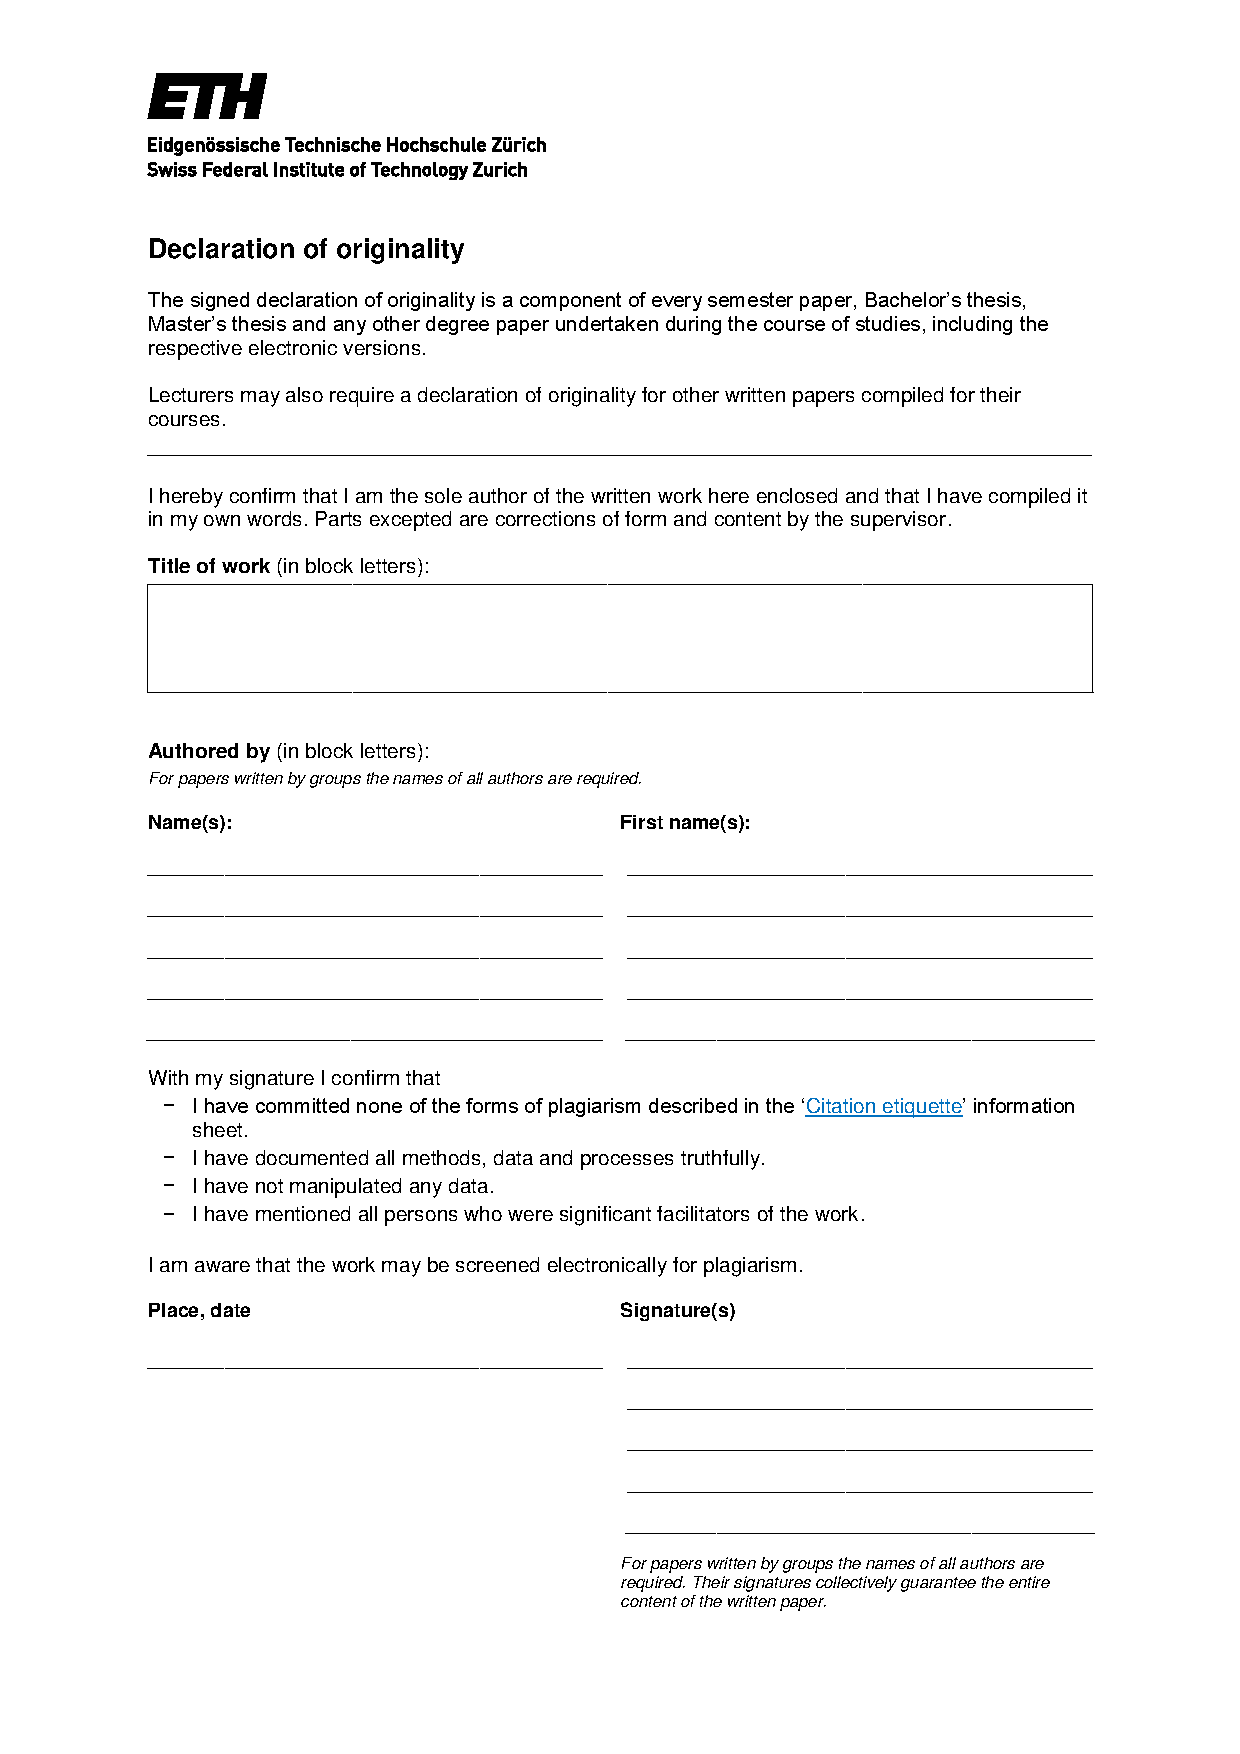
\includepdf[pages={1-},scale=1]{pdf/originality.pdf}

\end{document}
